\documentclass[12pt, a4paper]{ctexart}

% 导入常用宏包
\usepackage{geometry}
\geometry{left=2.5cm, right=2.5cm, top=2.5cm, bottom=2.5cm}
\usepackage{graphicx}
\usepackage{booktabs}
\usepackage{multirow}
\usepackage{amsmath}
\usepackage{float}
\usepackage{hyperref}
\usepackage{listings}
\usepackage{xcolor}
\usepackage{subcaption}
\usepackage{fontspec}
\newfontfamily\codefont{Consolas} 
% 代码块样式
\usepackage{listings}
\usepackage{xcolor}
\definecolor{tango-bg}{rgb}{0.97, 0.97, 0.97}
\definecolor{tango-comment}{rgb}{0.5, 0.5, 0.5}
\definecolor{tango-keyword}{rgb}{0.0, 0.0, 0.6}
\definecolor{tango-string}{rgb}{0.58, 0.0, 0.0}
\definecolor{tango-type}{rgb}{0.0, 0.3, 0.3}

\lstset{
    language=Python,
    backgroundcolor=\color{tango-bg},  % 浅灰色背景，看着不刺眼
    basicstyle=\codefont\small,        % 这里的 \ttfamily 就会自动调用上面的 Consolas
    commentstyle=\color{tango-comment}\itshape,
    keywordstyle=\color{tango-keyword}\bfseries,
    stringstyle=\color{tango-string},
    numberstyle=\tiny\color{tango-comment}, % 行号颜色
    numbers=left,                      % 行号放左边
    numbersep=8pt,                     % 行号与代码的间距
    breaklines=true,                   % 自动换行
    showstringspaces=false,            % 不显示字符串里的空格
    frame=single,                      % 加个边框
    rulecolor=\color{black!20},        % 边框颜色浅一点
    xleftmargin=1.5em,                 % 整体左侧缩进
    xrightmargin=1em,
    tabsize=4,                         % tab缩进
    captionpos=b,                      % 标题在下方
    aboveskip=1.5em,                   % 与上下文的距离
    belowskip=1em
}


\title{基于多传感器时间序列的液压设备故障诊断与状态监测系统}
\author{姓名：寇明睿 \quad 学号：3023244054 }
\date{\today}

\begin{document}

\maketitle

\begin{abstract}
本项目基于UCI液压系统状态监测数据集\cite{helwig2015}，利用14路多采样率传感器时间序列，构建了针对冷却器、阀门、泵、蓄能器的多输出故障诊断与告警系统。本文介绍了数据固定划分策略、基线模型(B0)的构建、基于阶段变化特征与物理交叉特征的改进方案(B1/B3)及其消融实验(B2/B4)。实验涵盖了10/30/60秒观测预算、五种鲁棒性测试条件以及告警逻辑验证。结果表明，改进方案有效解决了长窗口下阀门诊断退化的问题，且具备一定的抗噪能力。
\par\vspace{0.8em}\noindent\textbf{关键词：} 液压系统；故障诊断；多传感器时间序列；随机森林；前缀诊断；防抖告警
\end{abstract}

\section{问题定义与设备传感器含义}
本项目基本任务为面向工业液压设备的状态监测，利用压力、流量、温度、振动以及电机功率时间序列，完成冷却器、阀、泵和蓄能器四类部件的状态诊断。同时输出各个部件的状态等级、支持多个部件同时异常，并在工作周期内逐步更新诊断和告警。

数据集中包含原始多路过程信号，信号组共有14路实测信号，压力传感器为PS1-PS6，电机功率为EPS1，体积流量传感器为FS1和FS2，温度传感器为TS1-TS4，振动速度指标为VS1。共有四个部件作为独立诊断输出，即为冷却器、阀、泵与蓄能器，各自有三至四种不同状态和一种正常等级。此外有稳定标识反映当前是否达到静态条件用于结果分层。

需要强调，各部件输出的是离散的\textbf{状态等级代码}，而非概率或百分比：冷却器取 $\{3, 20, 100\}$、阀门取 $\{73, 80, 90, 100\}$、泵取 $\{0, 1, 2\}$、蓄能器取 $\{90, 100, 115, 130\}$，其中 100/100/0/130 分别为四部件的正常等级。例如阀门输出 90 表示其处于特定的状态代码 90，并不代表"90\% 正常度"；因此本文的准确率、F1 等指标均基于类别代码的一致性计算，不得将等级数值按比例解释。

\section{数据及独立划分}

\subsection{数据划分方案设计}
数据划分使用prepare.py实现，输出文件为manifest.csv，通过读入profile.txt，首先根据四个部件共计144种状态四元组组合进行分组并且提取样本，使用固定种子打乱，依照实验要求划分训练集、验证集、测试集。其中每个集合的组合数与周期数符合实验指导书要求，稳定性标志分布如下表所示：

\begin{table}[H]
    \centering
    \caption{稳定性标志在训练集、验证集和测试集中的分布}
    \label{tab:stable_flag_dist}
    \begin{tabular}{lccc}
        \toprule
        \textbf{stable\_flag} & \textbf{train} & \textbf{val} & \textbf{test} \\
        \midrule
        0                     & 860            & 290          & 299           \\
        1                     & 268            & 228          & 260           \\
        \bottomrule
    \end{tabular}
\end{table}

需要说明，训练集与验证集共同覆盖了大部分四元组组合，而测试集（29 组）仅由\textbf{未在训练/验证集中出现}的组合构成，并保留唯一的全正常组合（\texttt{100\_100\_0\_130}）用于误报检验。因此测试集评估的是模型在未见组合与全正常工况下的诊断与误报能力，而非对已见组合的记忆能力；这也与后文全正常组合误报率偏高的现象相互呼应。

\subsection{数据质量与多速率处理}
14路信号文件与profile.txt经逐行核对行数均为2205，周期一一对应，无缺行或错位。按各通道原始采样率统计，每周期样本数为：100Hz 通道（PS1--PS6、EPS1）6000点，10Hz通道（FS1、FS2）600点，1Hz 通道（TS1--TS4、VS1）60点，与60秒周期长度一致。

对全部通道进行非有限值检查，原始文件未发现NaN或Inf；对近常数通道以 $\sigma < 10^{-8}$ 判定，将其线性趋势斜率置为NaN并附加missing标记，避免把近零常数误当作有效物理量。各物理量单位以官方说明为准：压力为bar、电机功率为W、体积流量为L/min、温度为 $^\circ$C、振动速度指标为mm/s。

在采样率处理上，本系统不对信号做重采样：各通道在观测前缀内按自身原始采样率独立提取统计特征，不将 1Hz 信号复制为100Hz。处理前后数据规模保持一致：2205个原始周期按状态组合划分为训练1128、验证518、测试559，合计2205，与原始行数完全对应。每个周期在manifest.csv中记录周期编号、四部件标签、组合编号、稳定性标志、所属集合与原始行号，用于数据审计与结果分层。

\section{基线特征与四部件模型}
\subsection{时域统计特征}
基线模型使用各通道统计量作为特征，对于每个通道提取均值、标准差、最大值、最小值、均方根和线性趋势。对于一个传感器通道在观测窗口内的时间序列数据$X = \{x_1, x_2, \dots, x_N\}$，其中均值使用mean函数实现，数学公式为$$ \mu = \frac{1}{N} \sum_{i=1}^{N} x_i $$，反映传感器在观测窗口内的平均工作状态，即为工作基准点。标准差使用std函数实现，数学公式为$$ \sigma = \sqrt{\frac{1}{N-1} \sum_{i=1}^{N} (x_i - \mu)^2} $$，反映波动强度或噪声水平，衡量数据围绕均值的离散程度。最大值和最小值使用max和min函数实现，分别计算公式为$ x_{\max} = \max_{i} (x_i) $和$x_{\min} = \min_{i} (x_i) $，分别表示上极限状态和下极限状态，为观测窗口内的瞬时极值。均方根使用sqrt函数计算，数学公式为$$ x_{\text{rms}} = \sqrt{\frac{1}{N} \sum_{i=1}^{N} x_i^2} $$。反映有效能量或者总体强度，线性趋势计算线性回归斜率，数学公式为$$ k = \frac{N \sum_{i=1}^{N} x_i t_i - \left(\sum_{i=1}^{N} x_i\right) \left(\sum_{i=1}^{N} t_i\right)}{N \sum_{i=1}^{N} t_i^2 - \left(\sum_{i=1}^{N} t_i\right)^2} $$，反映变化方向和速率，反映信号在观测窗口内随时间变化的长期走向。计算结果拼接作为当前时间窗口的特征。对于每个模型记录元数据，包括时间预算、随机种子、通道映射名称和补偿中位数，近常数判定规则。
\subsection{多输出随机森林与缺失补偿}
对于四个部件使用独立的随机森林进行计算，使用sklearn中的RandomForestClassifier进行拟合，树的数目为200。对于近常数通道使用标准差小于$10^{-8}$进行判断，近常数通道的线性趋势使用无穷大替换并加入近常数标记作为特征。

缺失补偿使用当前训练集的中位数进行补偿，使用nanmedian计算，中位数具有稳健性，对于异常值不敏感，可以有效的代表数据的中心趋势和典型工作状态，同时保持填充值和原始数据量纲一致。对于缺失数据进行保留，使用额外的二进制列对于每个通道记录是否缺失，统一加入特征矩阵中。后文以B0基线模型指代此方案。

\section{前缀诊断与告警逻辑}
\subsection{观测预算设计}
使用三种观测预算，分别为10秒，30秒和60秒，表示周期开始后的前若干秒，即为观测前缀，对于各个时间预算报告相应四部件诊断和逐类召回，30秒需要验证相对10秒是否更加可靠，完整周期60秒作为主要状态诊断结果。每个时间预算分别训练模型和特征处理参数，只能使用时间预算内的数据形成特征矩阵。具体实现中伪代码如下，仅截取到达时间预算戳前的数据。
\begin{lstlisting}[language=Python, caption=前缀观测数据截取核心逻辑]
def extract_prefix(raw, fs, seconds):
    n_use = int(fs * seconds)
    # 严格截取前缀，绝不使用未来数据
    x = raw[:, :n_use]
    return x
\end{lstlisting}
\subsection{防抖告警设计}
状态诊断与告警输出种每个时间节点输出四个部件各自的等级和类别得分，对于非正常等级的诊断先判定为异常候选，同一部件在连续两个输出时点预测为相同的非正常等级时发出一次正式告警，每个周期不重复计数仅告警一次，周期结束后重置状态。可以有效过滤瞬态噪声防止过多误报。具体实现中伪代码如下:
\begin{lstlisting}[language=Python, caption=连续双时点防抖告警状态机]
def check_alarm(predictions, normal_levels):
    candidates = {}  # 记录候选状态
    alarms = []      # 记录正式告警
    for time_step, preds in predictions:
        for comp, level in preds.items():
            # 状态恢复：如果预测为正常，清除该部件的历史候选
            if level == normal_levels[comp]:
                candidates.pop(comp, None)
                continue
            # 状态触发：如果预测异常
            if comp not in candidates:
                candidates[comp] = (level, time_step) # 首次异常，加入候选
            elif candidates[comp][0] == level:
                # 连续两个时点预测为同一非正常等级，正式告警
                alarms.append({
                    "component": comp, 
                    "time": time_step, 
                    "level": level
                })
                # 触发后移出候选池，保证同一周期最多告警一次
                del candidates[comp] 
    return alarms
\end{lstlisting}
\subsection{周期边界处理}
每个负载周期视为独立试验单元。回放与批量评测时，周期切换后须重置历史候选状态、告警计数与统计量，避免把上一周期的诊断上下文带入下一周期。因此，本系统不将多个周期拼接后产生的标签变化解释为设备从正常到故障的真实演化过程，各周期之间不存在状态延续关系。

\section{失败分析与改进消融}
\subsection{基线失败分析}
下图展示四个部件在基线模型上的混淆矩阵，反映如下问题和可能改进方向。
\begin{figure}[H]
    \centering
    % 第一行两张子图
    \begin{subfigure}[b]{0.45\textwidth}
        \centering
        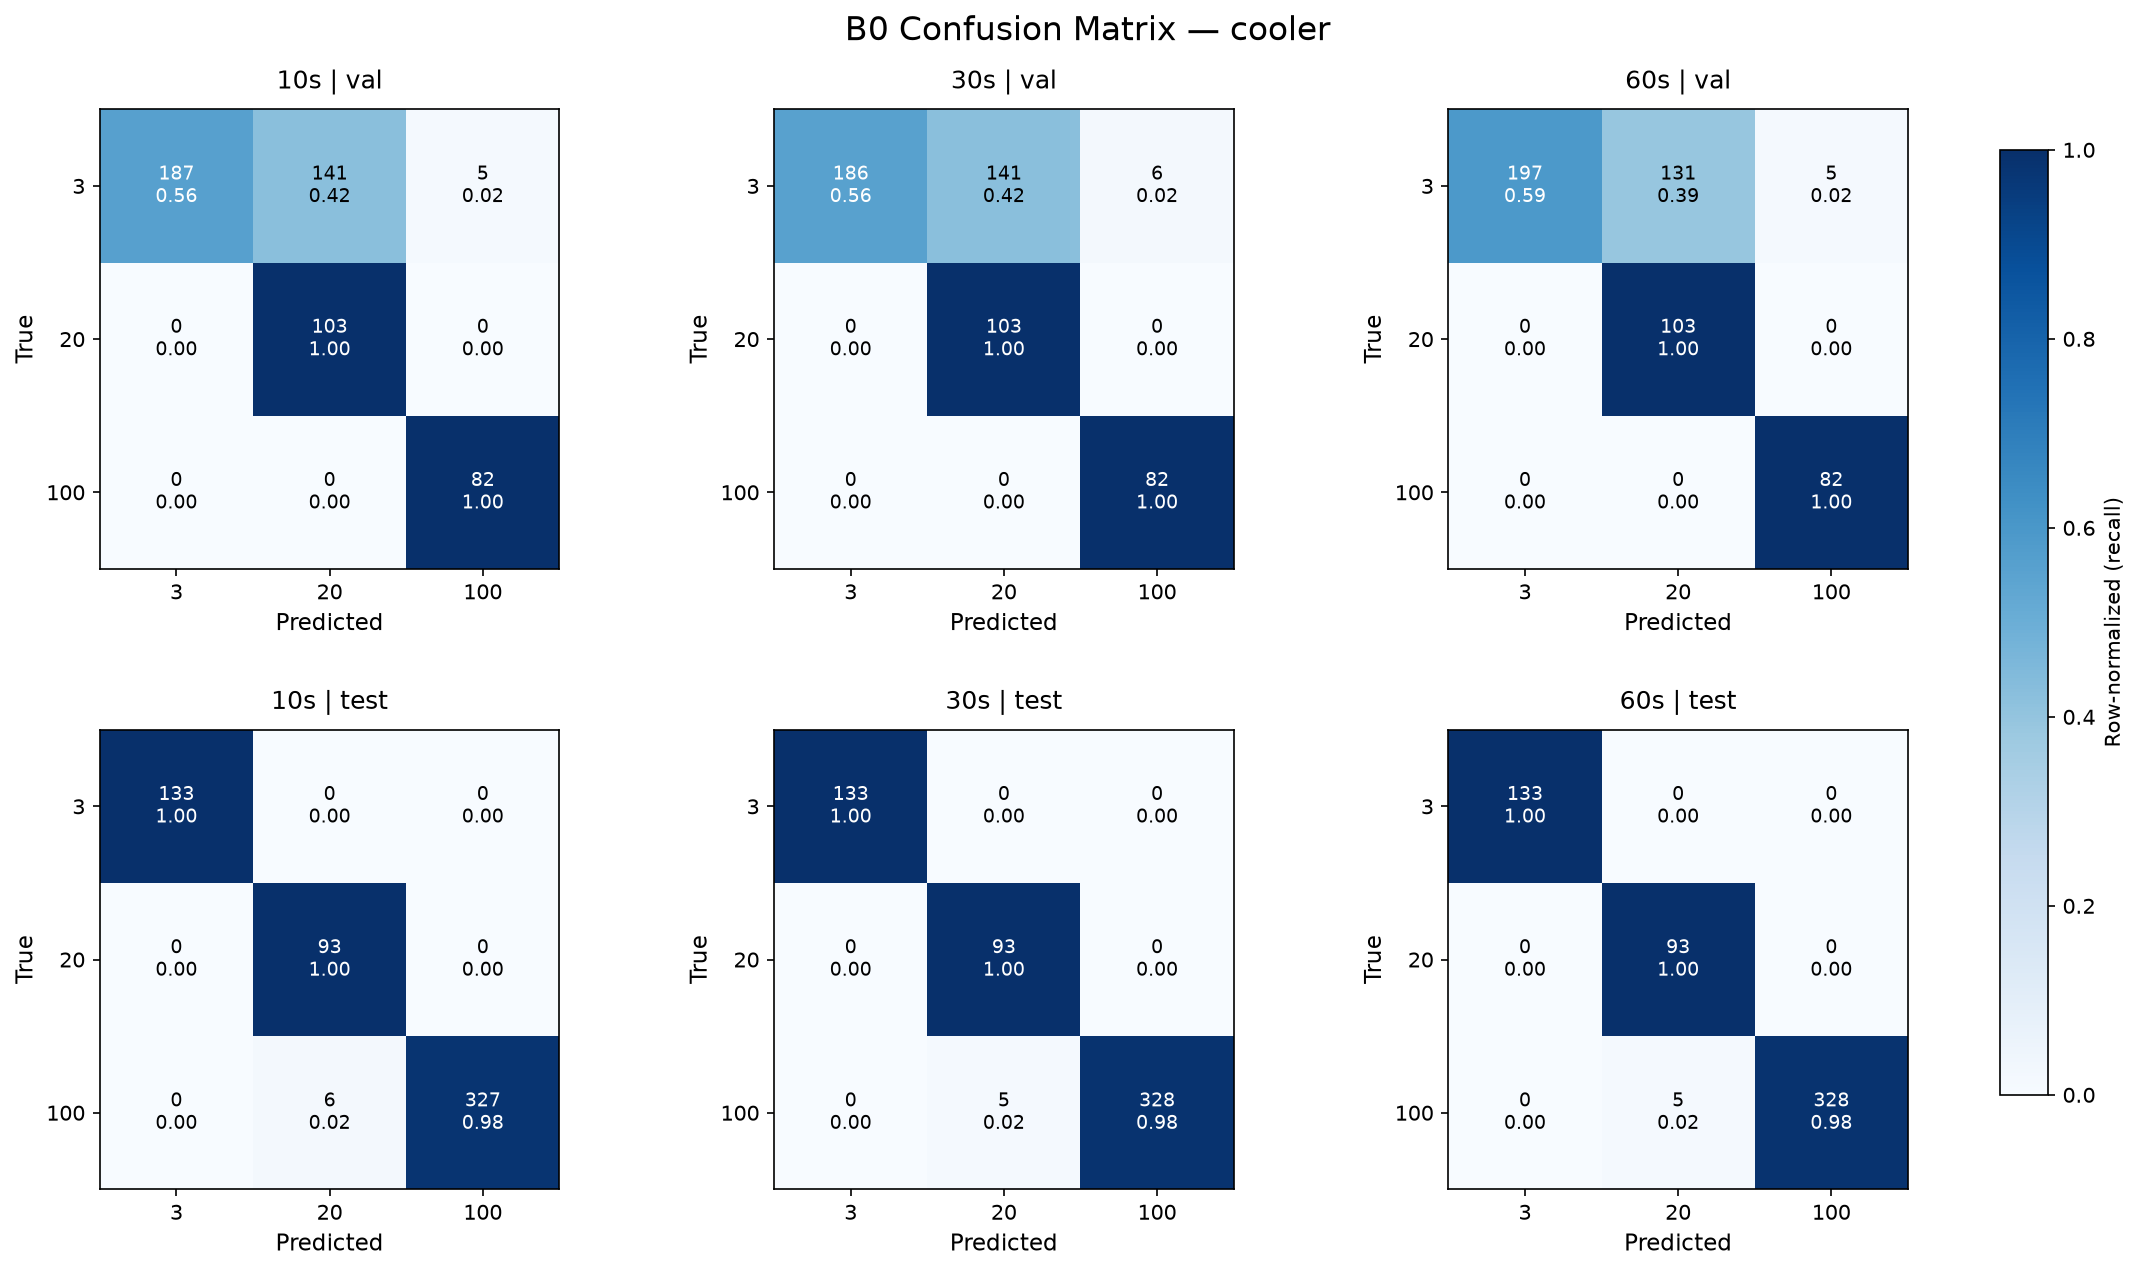
\includegraphics[width=\textwidth]{figures/cm_b0_cooler.png}
        \caption{冷却器部件混淆矩阵}
        \label{fig:cm_b0_cooler}
    \end{subfigure}
    \hfill
    \begin{subfigure}[b]{0.45\textwidth}
        \centering
        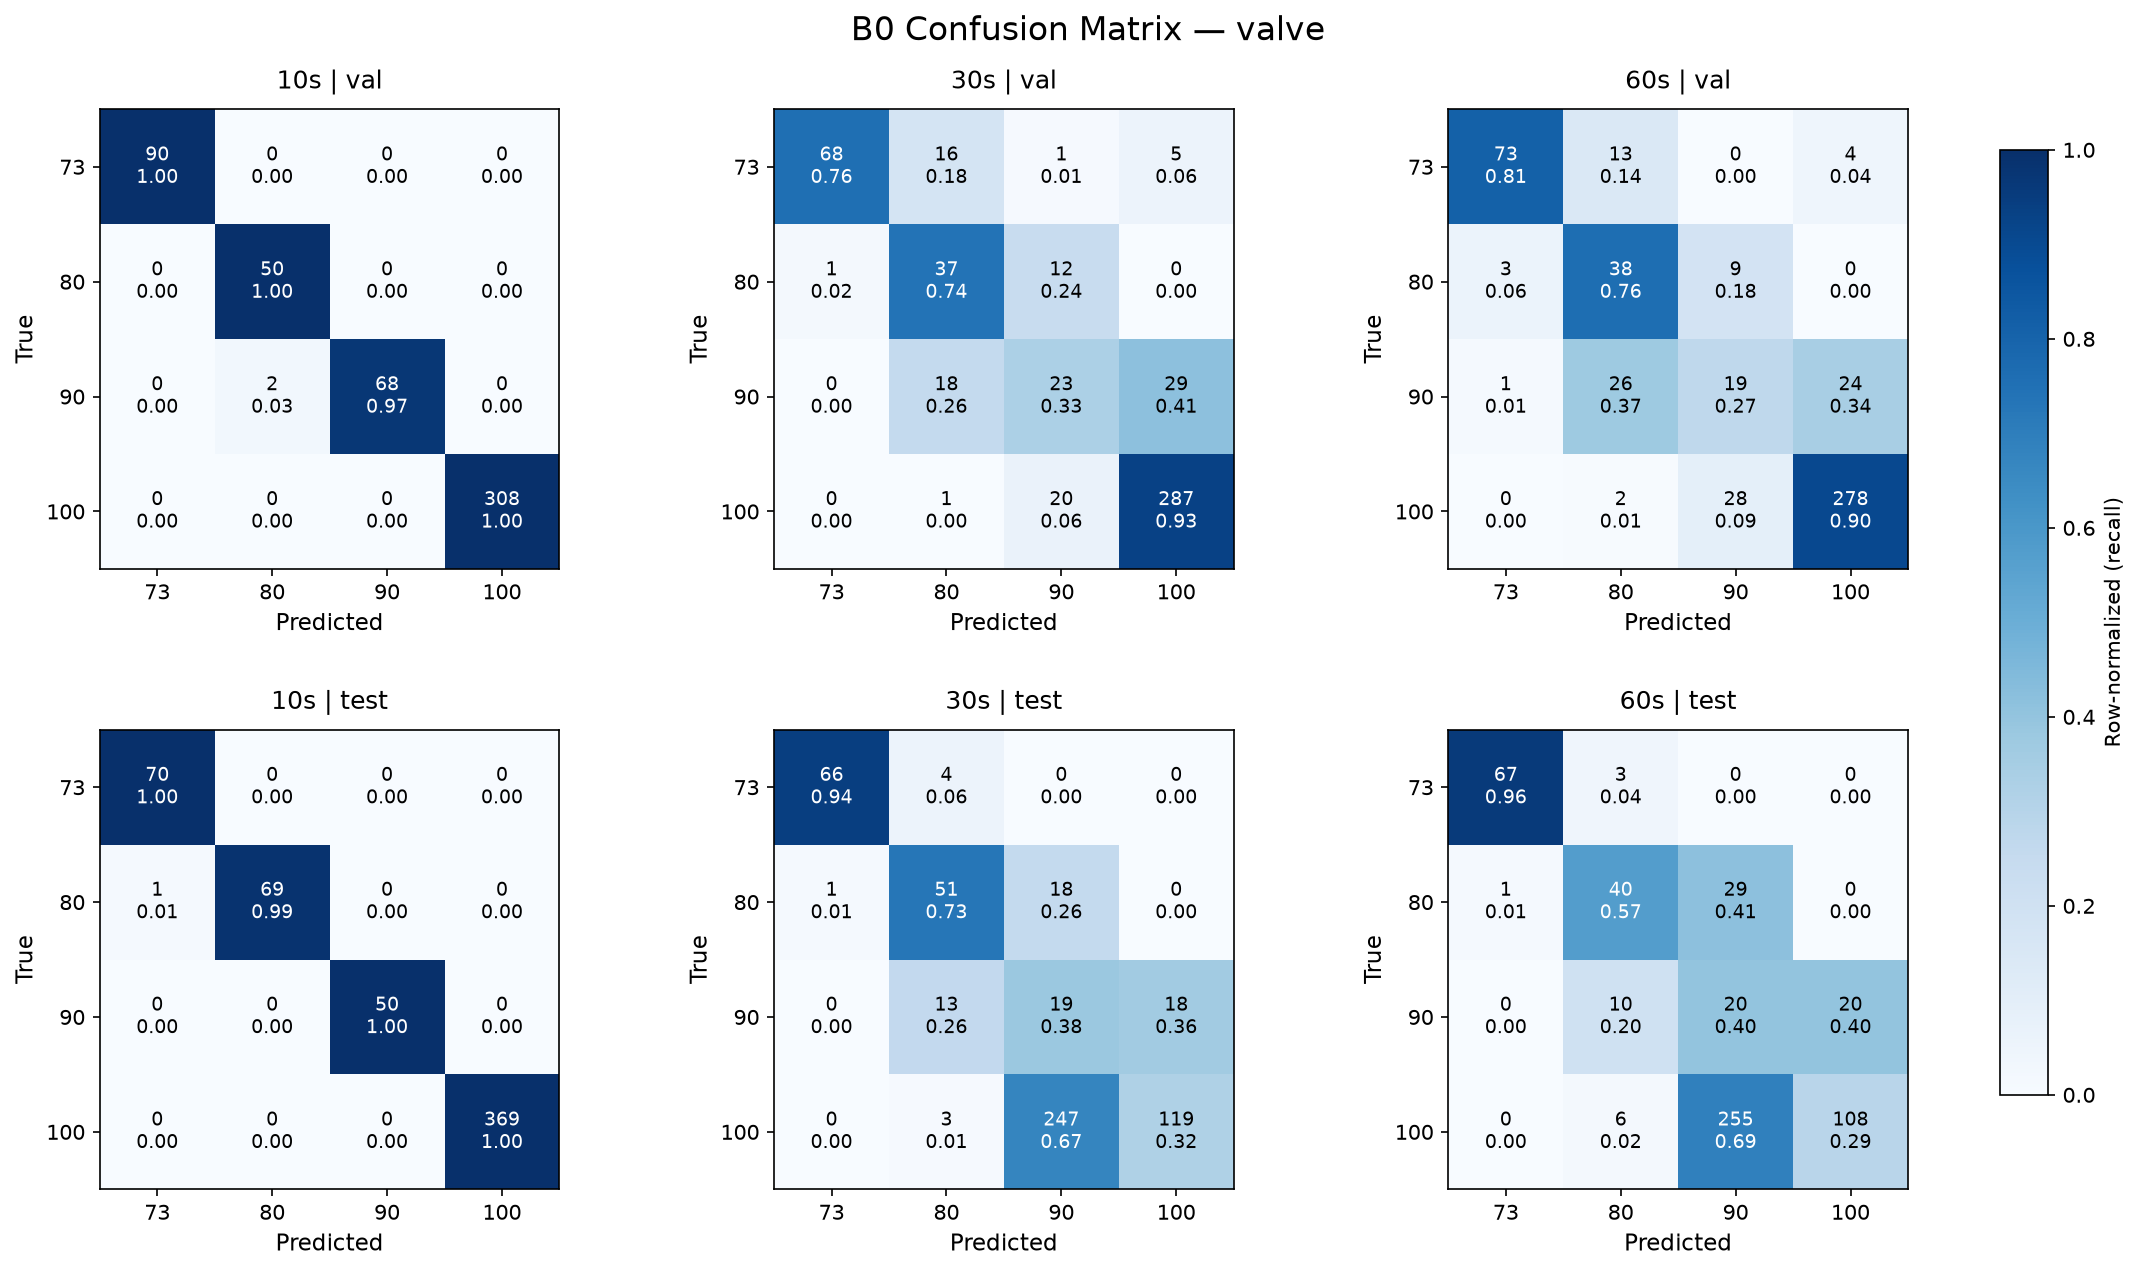
\includegraphics[width=\textwidth]{figures/cm_b0_valve.png}
        \caption{阀门部件混淆矩阵}
        \label{fig:cm_b0_valve}
    \end{subfigure}
    
    % 第二行两张子图
    \vspace{0.5cm}
    \begin{subfigure}[b]{0.45\textwidth}
        \centering
        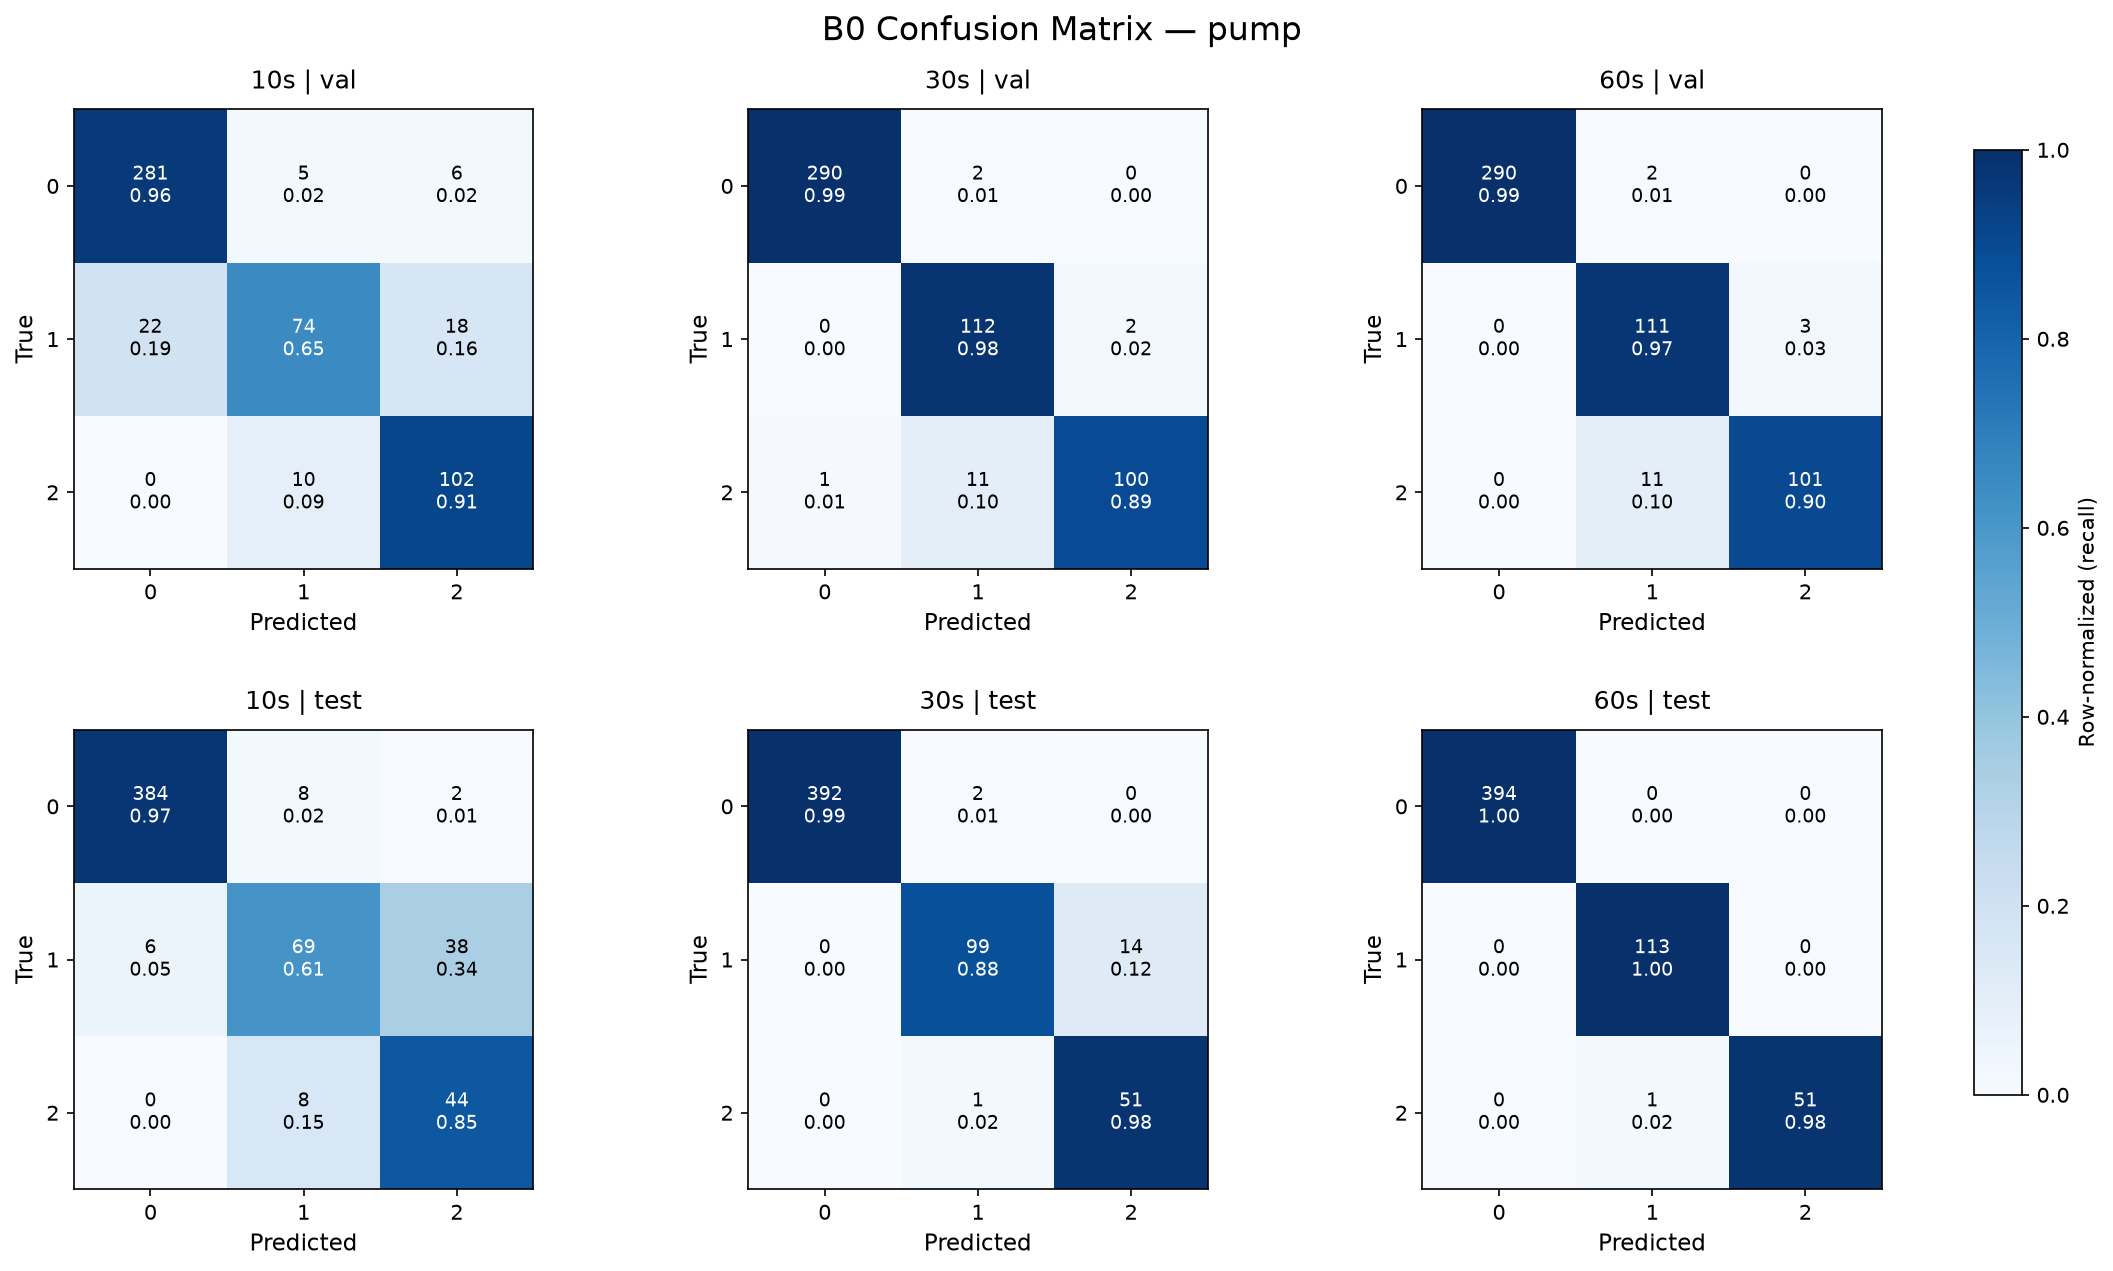
\includegraphics[width=\textwidth]{figures/cm_b0_pump.png}
        \caption{泵部件混淆矩阵}
        \label{fig:cm_b0_pump}
    \end{subfigure}
    \hfill
    \begin{subfigure}[b]{0.45\textwidth}
        \centering
        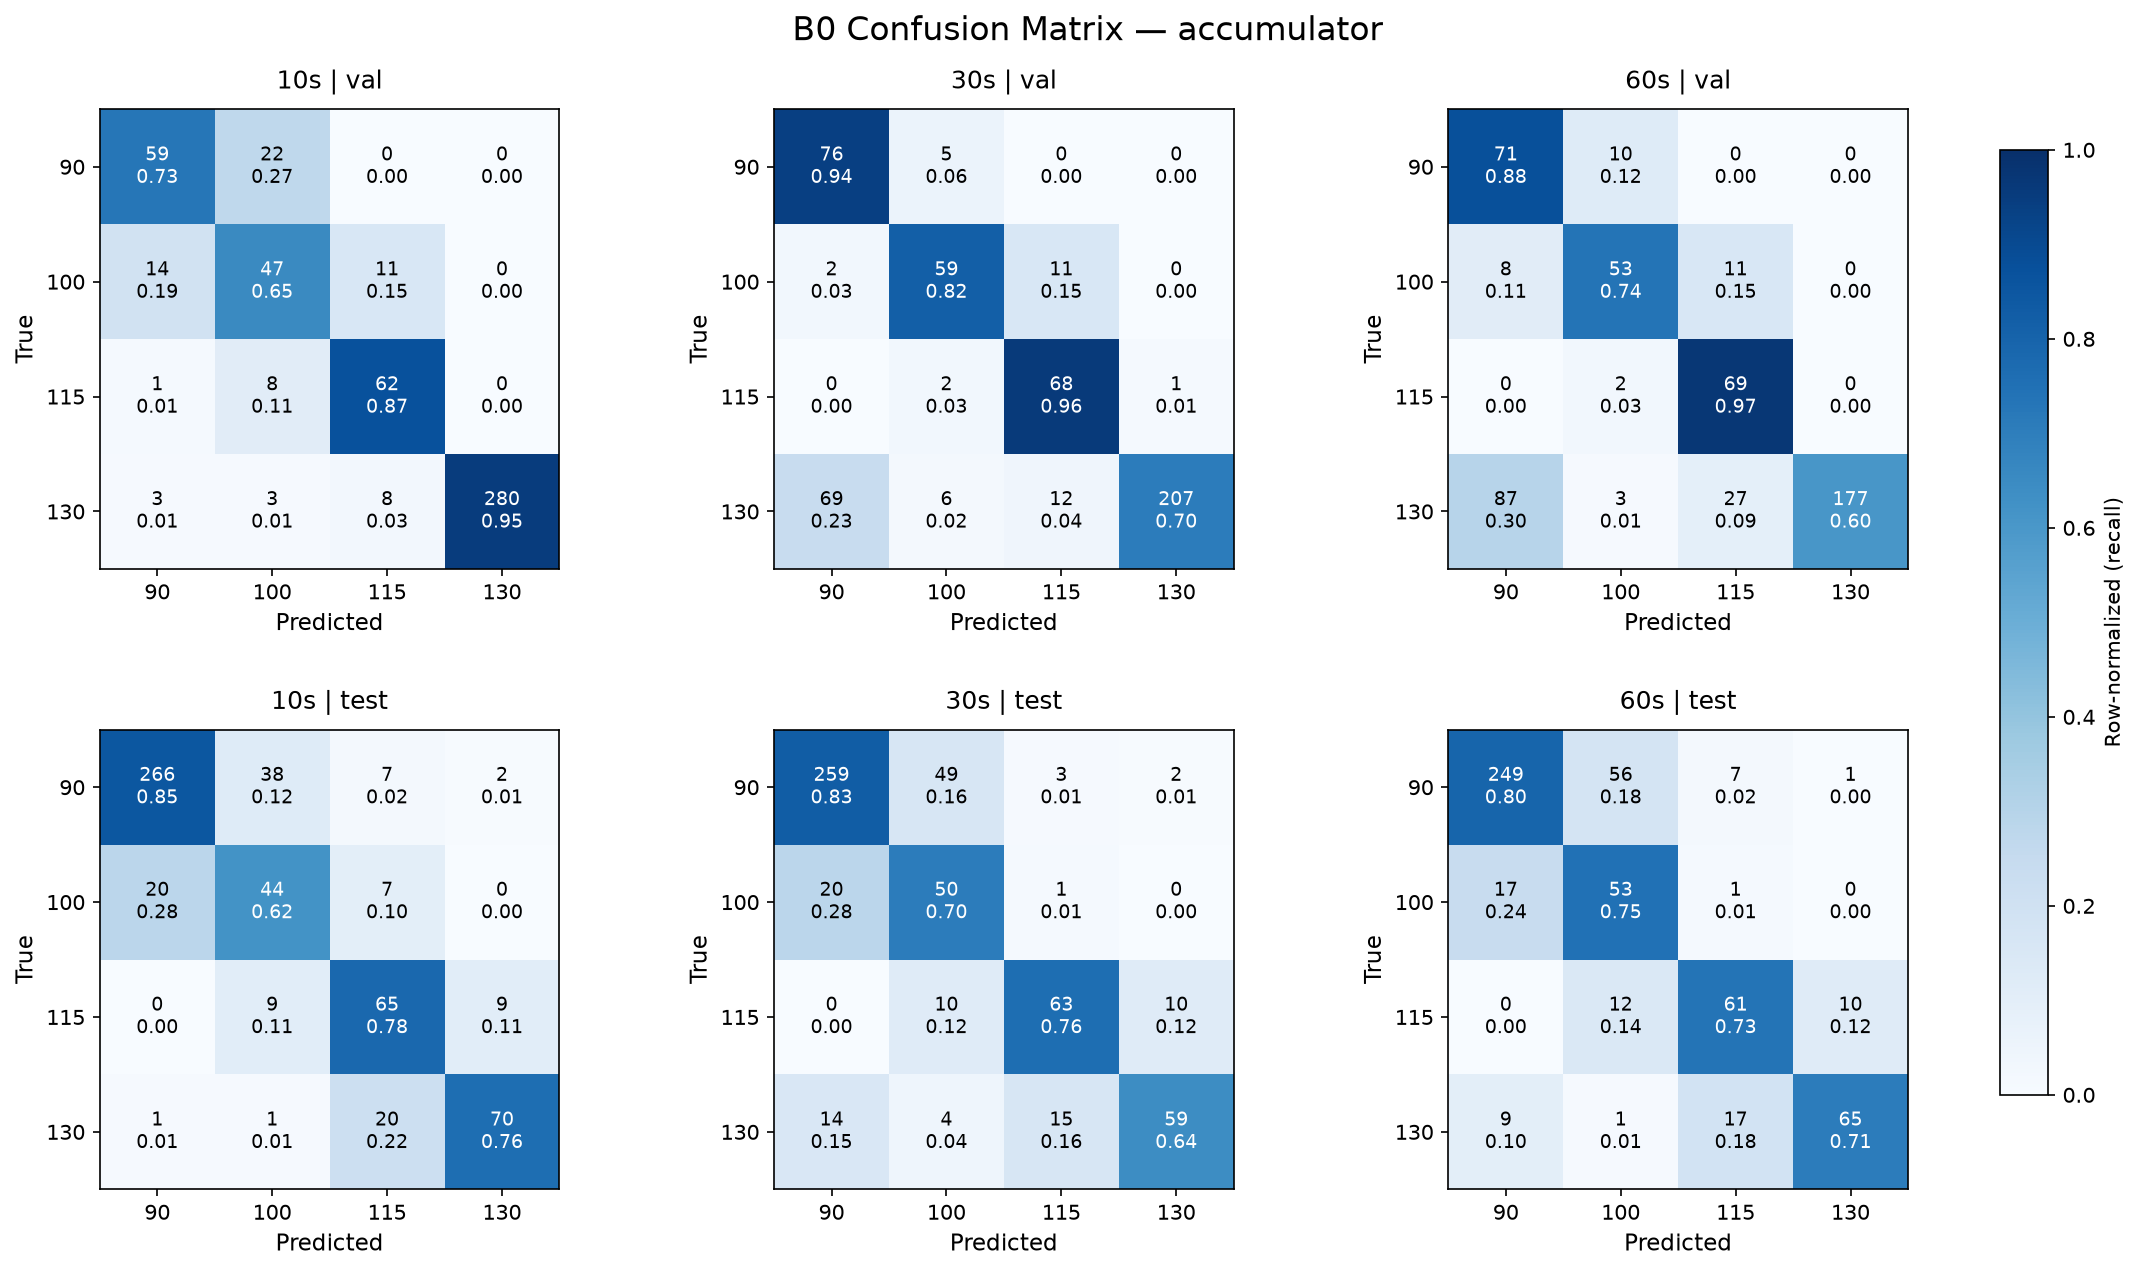
\includegraphics[width=\textwidth]{figures/cm_b0_accumulator.png}
        \caption{蓄能器部件混淆矩阵}
        \label{fig:cm_b0_accumulator}
    \end{subfigure}
    
    % 总标题与总标签
    \caption{基线模型下四个液压部件的混淆矩阵对比}
    \label{fig:b0_all_confusion}
\end{figure}

冷却器在三种时间预算上召回率几乎不变，并且在较短时间预算（10秒）的测试集已经取得较好结果。对应冷却器变化状态较慢，温度类信号在10秒内已经足够判断，符合物理直觉。

泵部件在10秒上表现较差，较长时间预算上表现更好，可能反映泵的轻微内泄露是累积效应，较短时间预算无法充分展现，符合段时间窗口信息不足的直觉。

蓄能器在三个时间预算上表现接近，压力等级在较短的10秒内已经可以判别，主要混淆等级一直存在。

阀门部件出现反常状况。在较长时间预算（60秒）上召回率非常低，在较小时间预算（10秒）上几乎全对，可能原因在于阀的状态判别信息集中在周期早期，完整周期的全局均值和标准差将早期差异平均化后被掩盖，反映出阀的故障模式是切换滞后，切换动作发生在周期开始阶段，10秒的时间窗口恰好覆盖这个瞬态，标准差、线性趋势斜率对于这个瞬态较为敏感，完整周期内瞬态占比较小，均值和标准差被后续稳态稀释，全局统计量变得接近，模型无法分清不同状态标签。
\subsection{分段统计与差分特征引入}
\subsubsection{具体实现方法}
相对于基础的时域统计，改进方案引入时间维度的变化信息，目标是解决长窗口下因为信号平均化导致的故障特征丢失问题。引入分段均值和差分特征中具体加入五个额外的特征通道，划分60秒完整周期为三个20秒的分段，计算其各自均值和相邻两段之间的差值作为差分。具体伪代码如下：
\begin{lstlisting}[language=Python, caption={分段均值与差分特征计算逻辑}]
# 输入: x 为形状 (n_samples, n_timepoints) 的数组
n = x.shape[1]
# 初始化特征变量
seg_means = np.zeros((x.shape[0], 3))
diffs = np.zeros((x.shape[0], 2))
if n >= 15:
    # 等长分段 (取整)
    seg_len = n // 3
    s1 = x[:, :seg_len]
    s2 = x[:, seg_len : 2*seg_len]
    s3 = x[:, 2*seg_len : 3*seg_len]
    # 计算各段均值 (沿时间轴平均)
    mu1 = s1.mean(axis=1)
    mu2 = s2.mean(axis=1)
    mu3 = s3.mean(axis=1)
    # 组装分段均值特征
    seg_means = np.column_stack([mu1, mu2, mu3])
    # 计算相邻阶段的一阶差分
    diffs[:, 0] = mu1 - mu2  # 前段-中段
    diffs[:, 1] = mu2 - mu3  # 中段-后段
# 返回特征: 若窗口过短，则返回全零特征
return seg_means, diffs
\end{lstlisting}
两个差分标记直接反映信号在前、中、后三个阶段的变化率，有效增加动态敏感性，尤其是对于阀门这种执行部件，其状态体现在动作过程中的变化轨迹上，分段差分可以更好的刻画这种过程特征。具体实现中对于较短时间预算填充全部特征为0，进行统一处理。后文以B1方案指代引入分段统计与差分特征的方案。
\subsubsection{具体结果分析}
下图展示在引入分段统计与差分特征后四个部件的混淆矩阵示意图。
\begin{figure}[H]
    \centering
    % 第一行两张子图
    \begin{subfigure}[b]{0.45\textwidth}
        \centering
        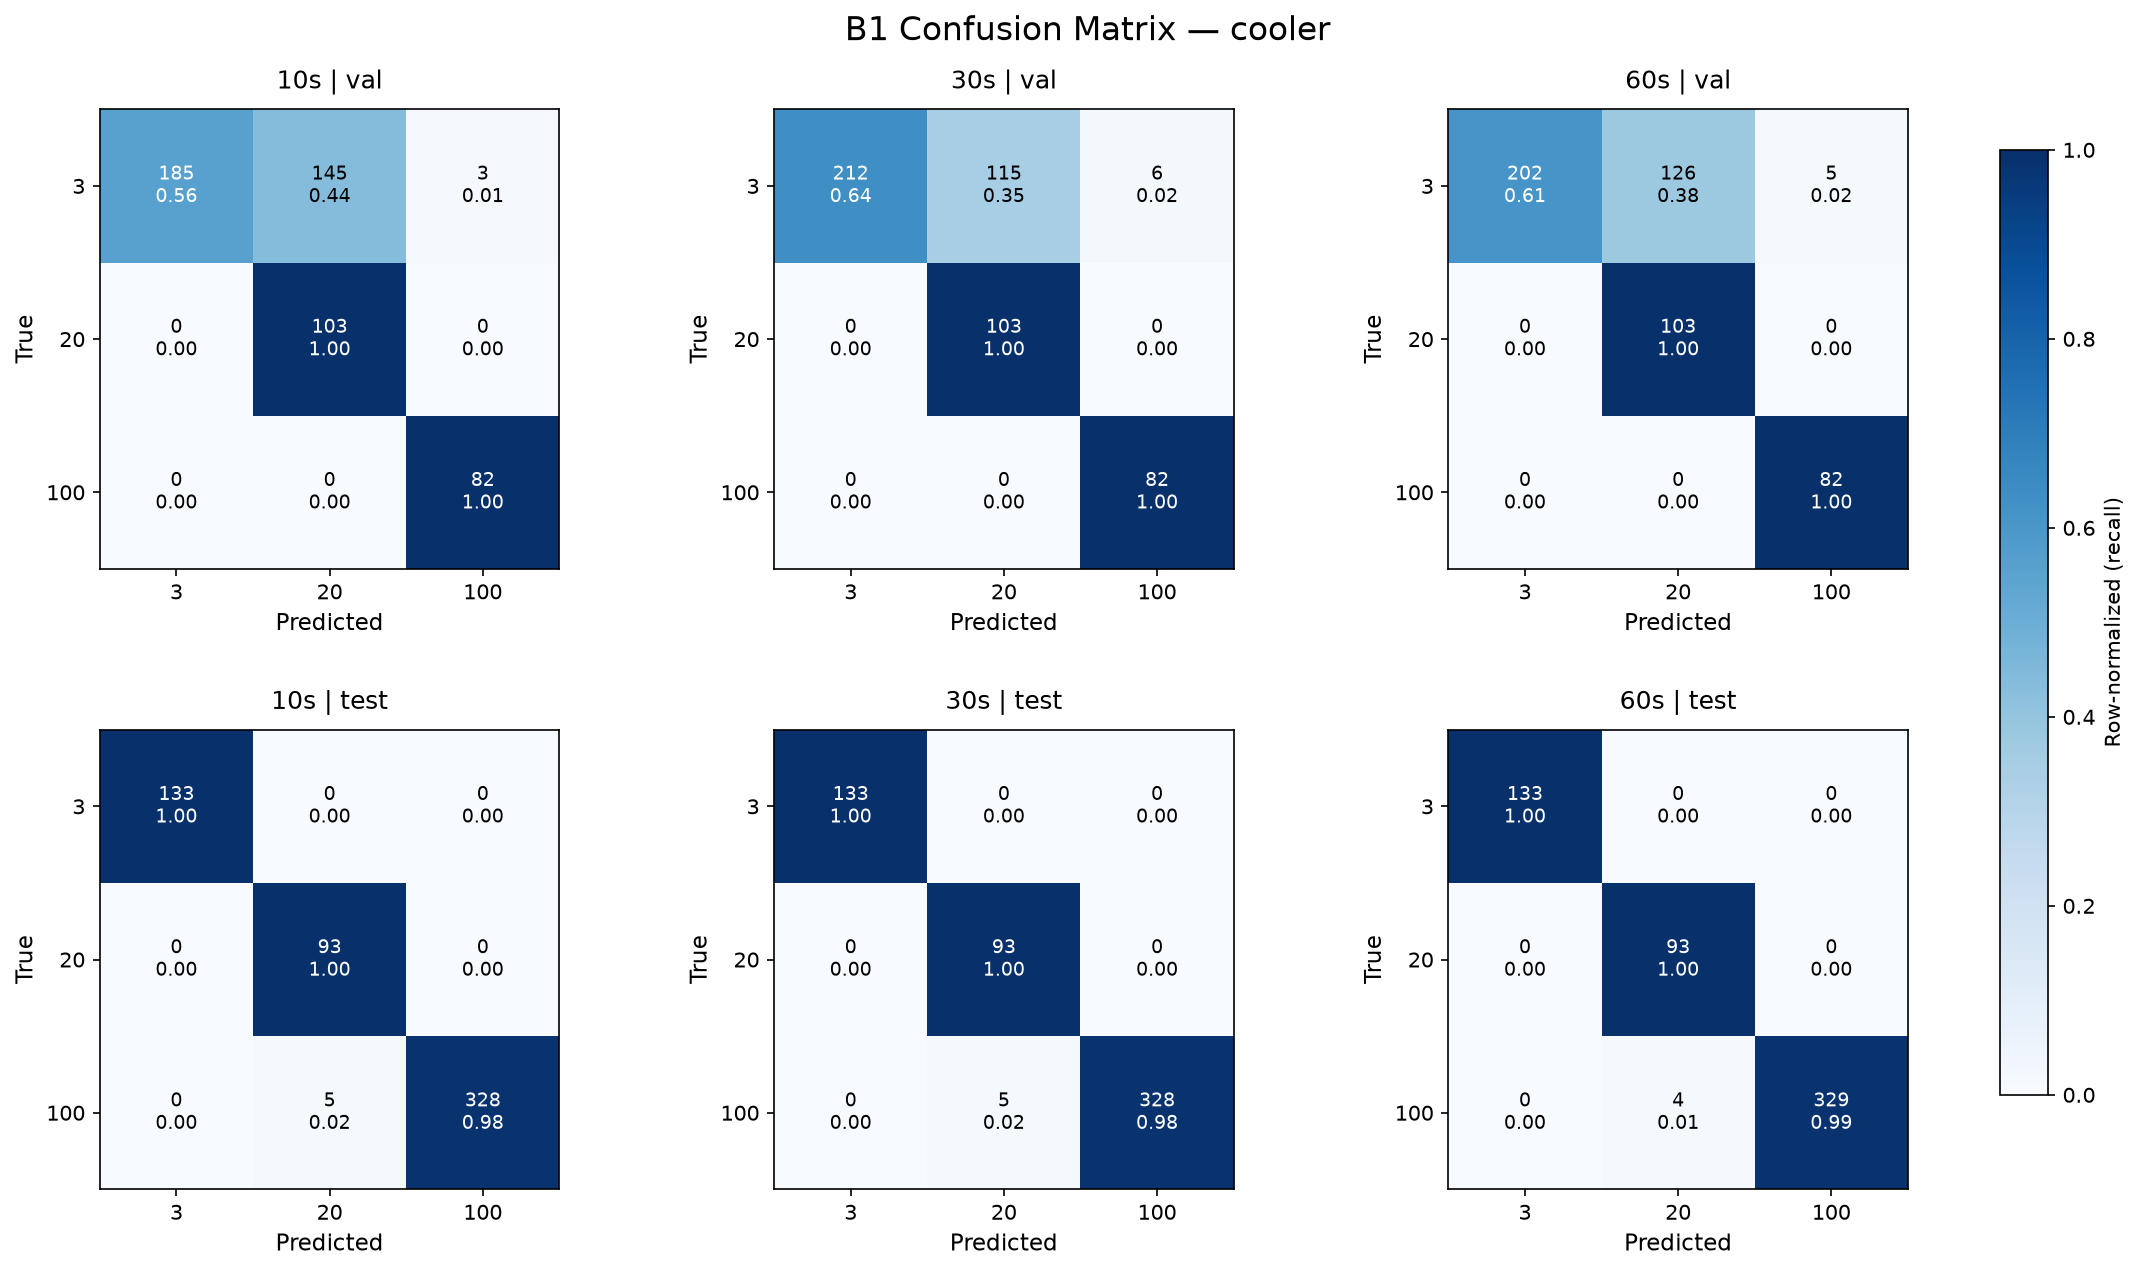
\includegraphics[width=\textwidth]{figures/cm_b1_cooler.png}
        \caption{冷却器部件混淆矩阵}
        \label{fig:cm_b1_cooler}
    \end{subfigure}
    \hfill
    \begin{subfigure}[b]{0.45\textwidth}
        \centering
        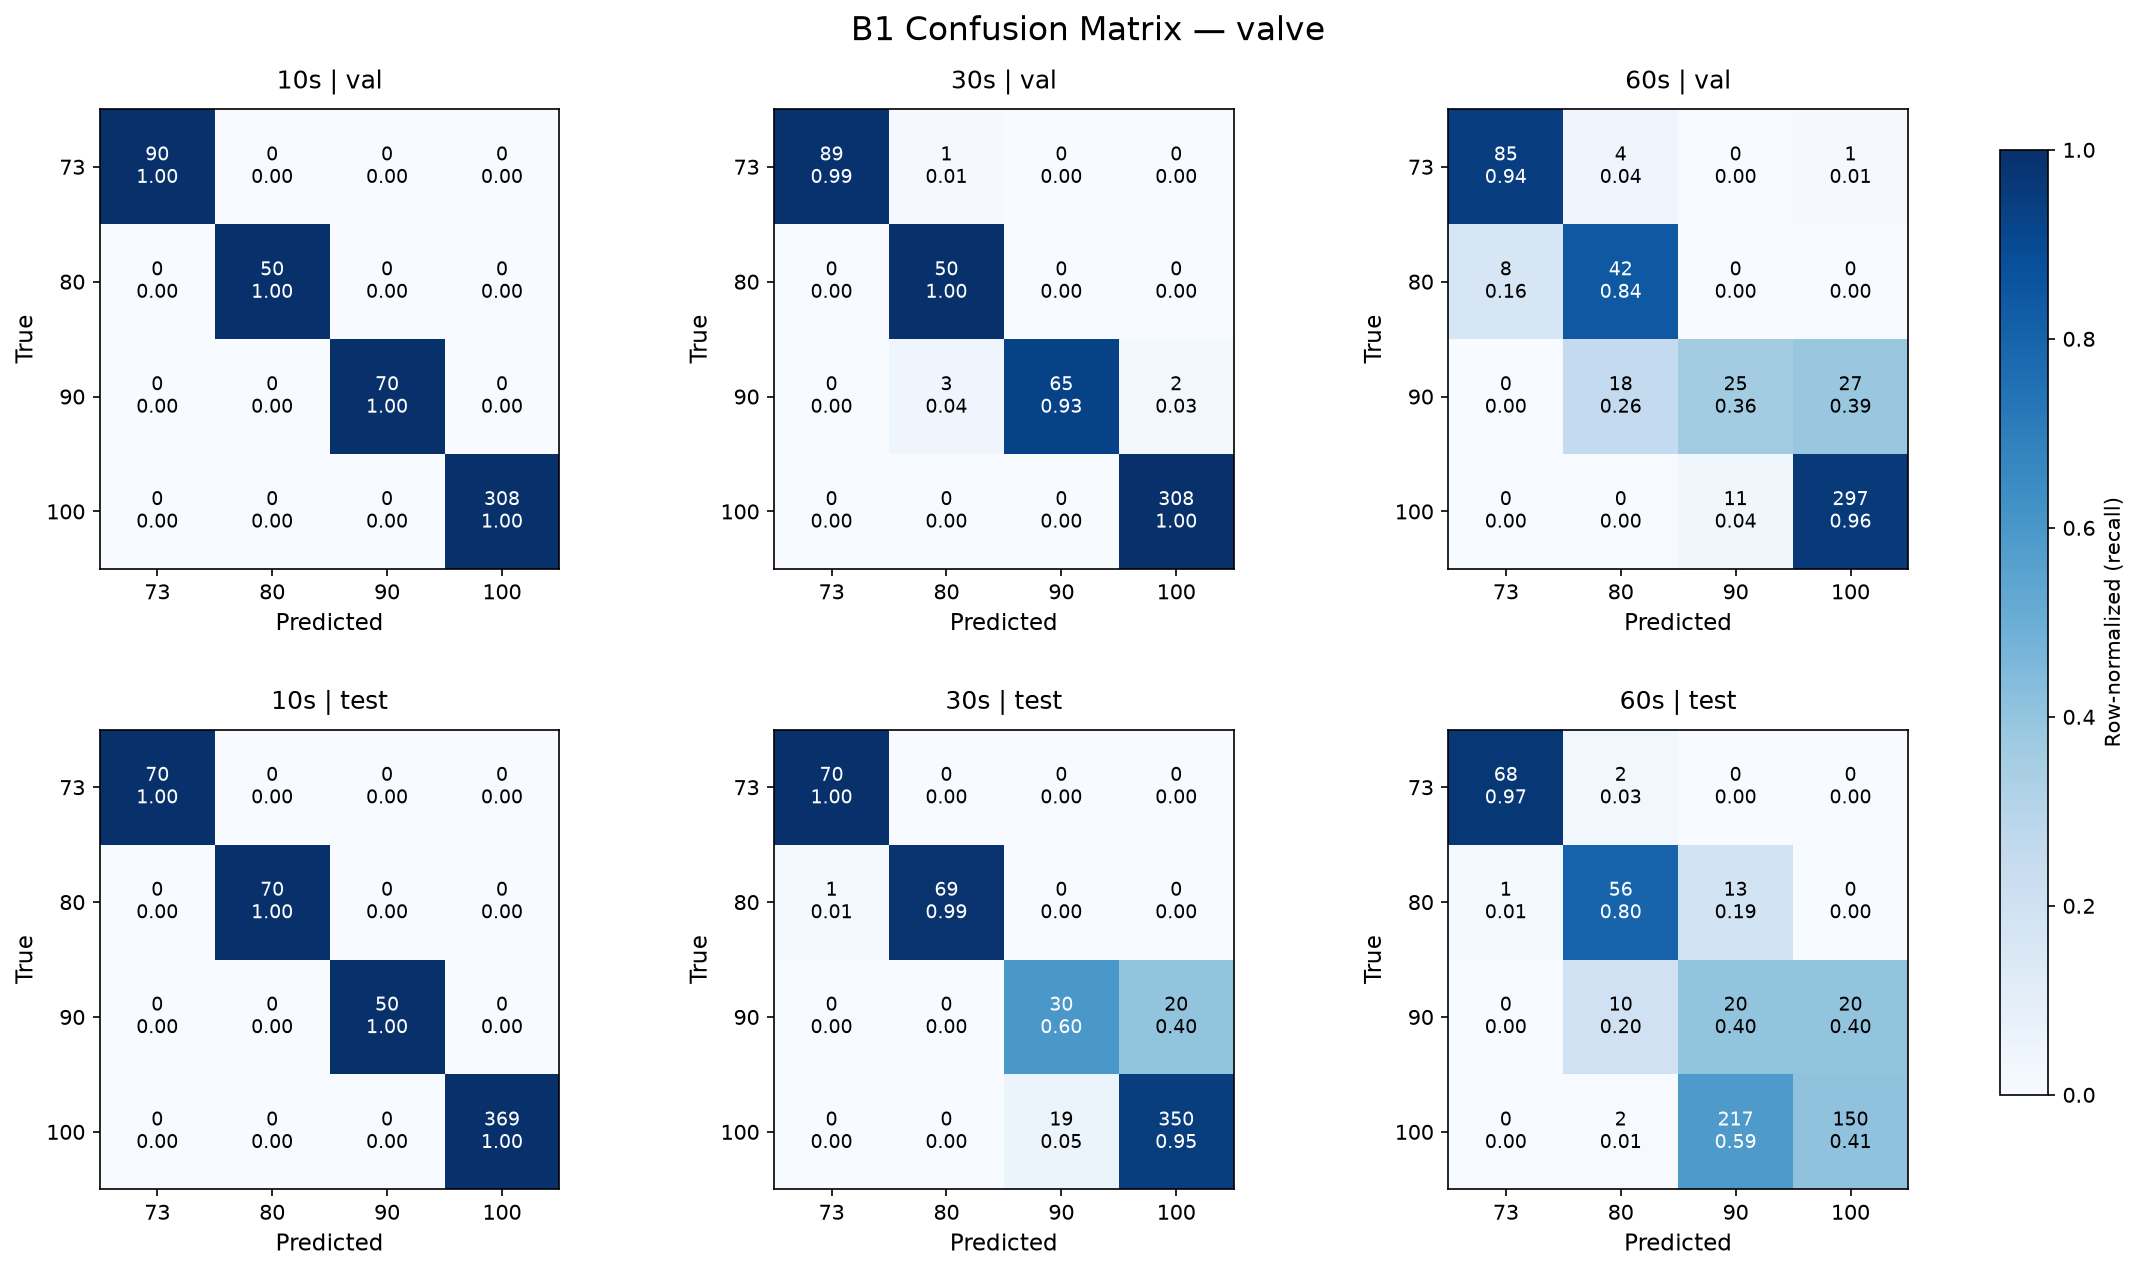
\includegraphics[width=\textwidth]{figures/cm_b1_valve.png}
        \caption{阀门部件混淆矩阵}
        \label{fig:cm_b1_valve}
    \end{subfigure}
    
    % 第二行两张子图
    \vspace{0.5cm}
    \begin{subfigure}[b]{0.45\textwidth}
        \centering
        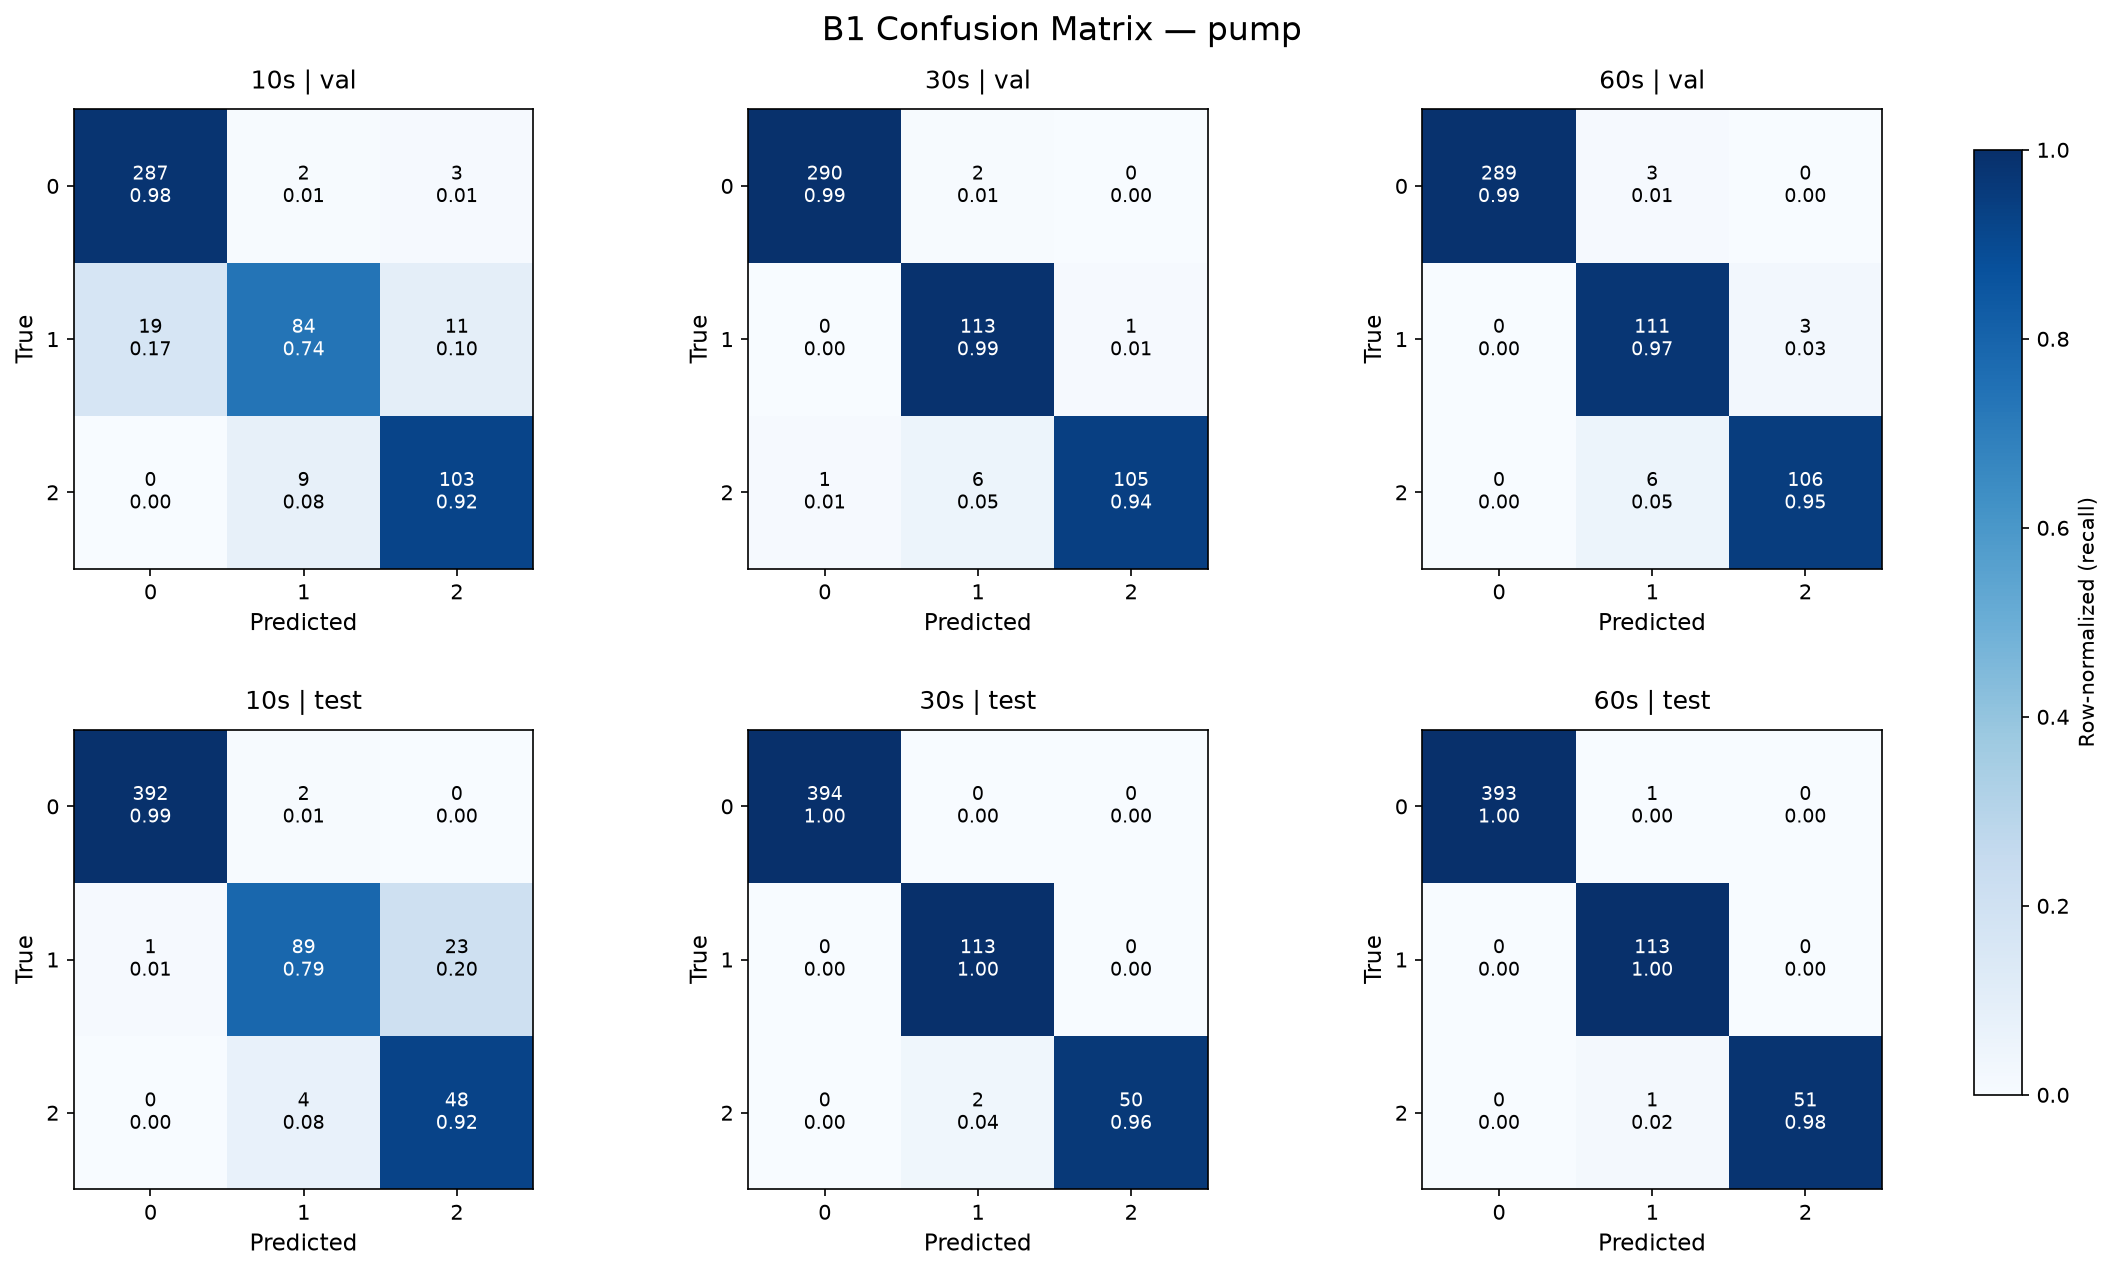
\includegraphics[width=\textwidth]{figures/cm_b1_pump.png}
        \caption{泵部件混淆矩阵}
        \label{fig:cm_b1_pump}
    \end{subfigure}
    \hfill
    \begin{subfigure}[b]{0.45\textwidth}
        \centering
        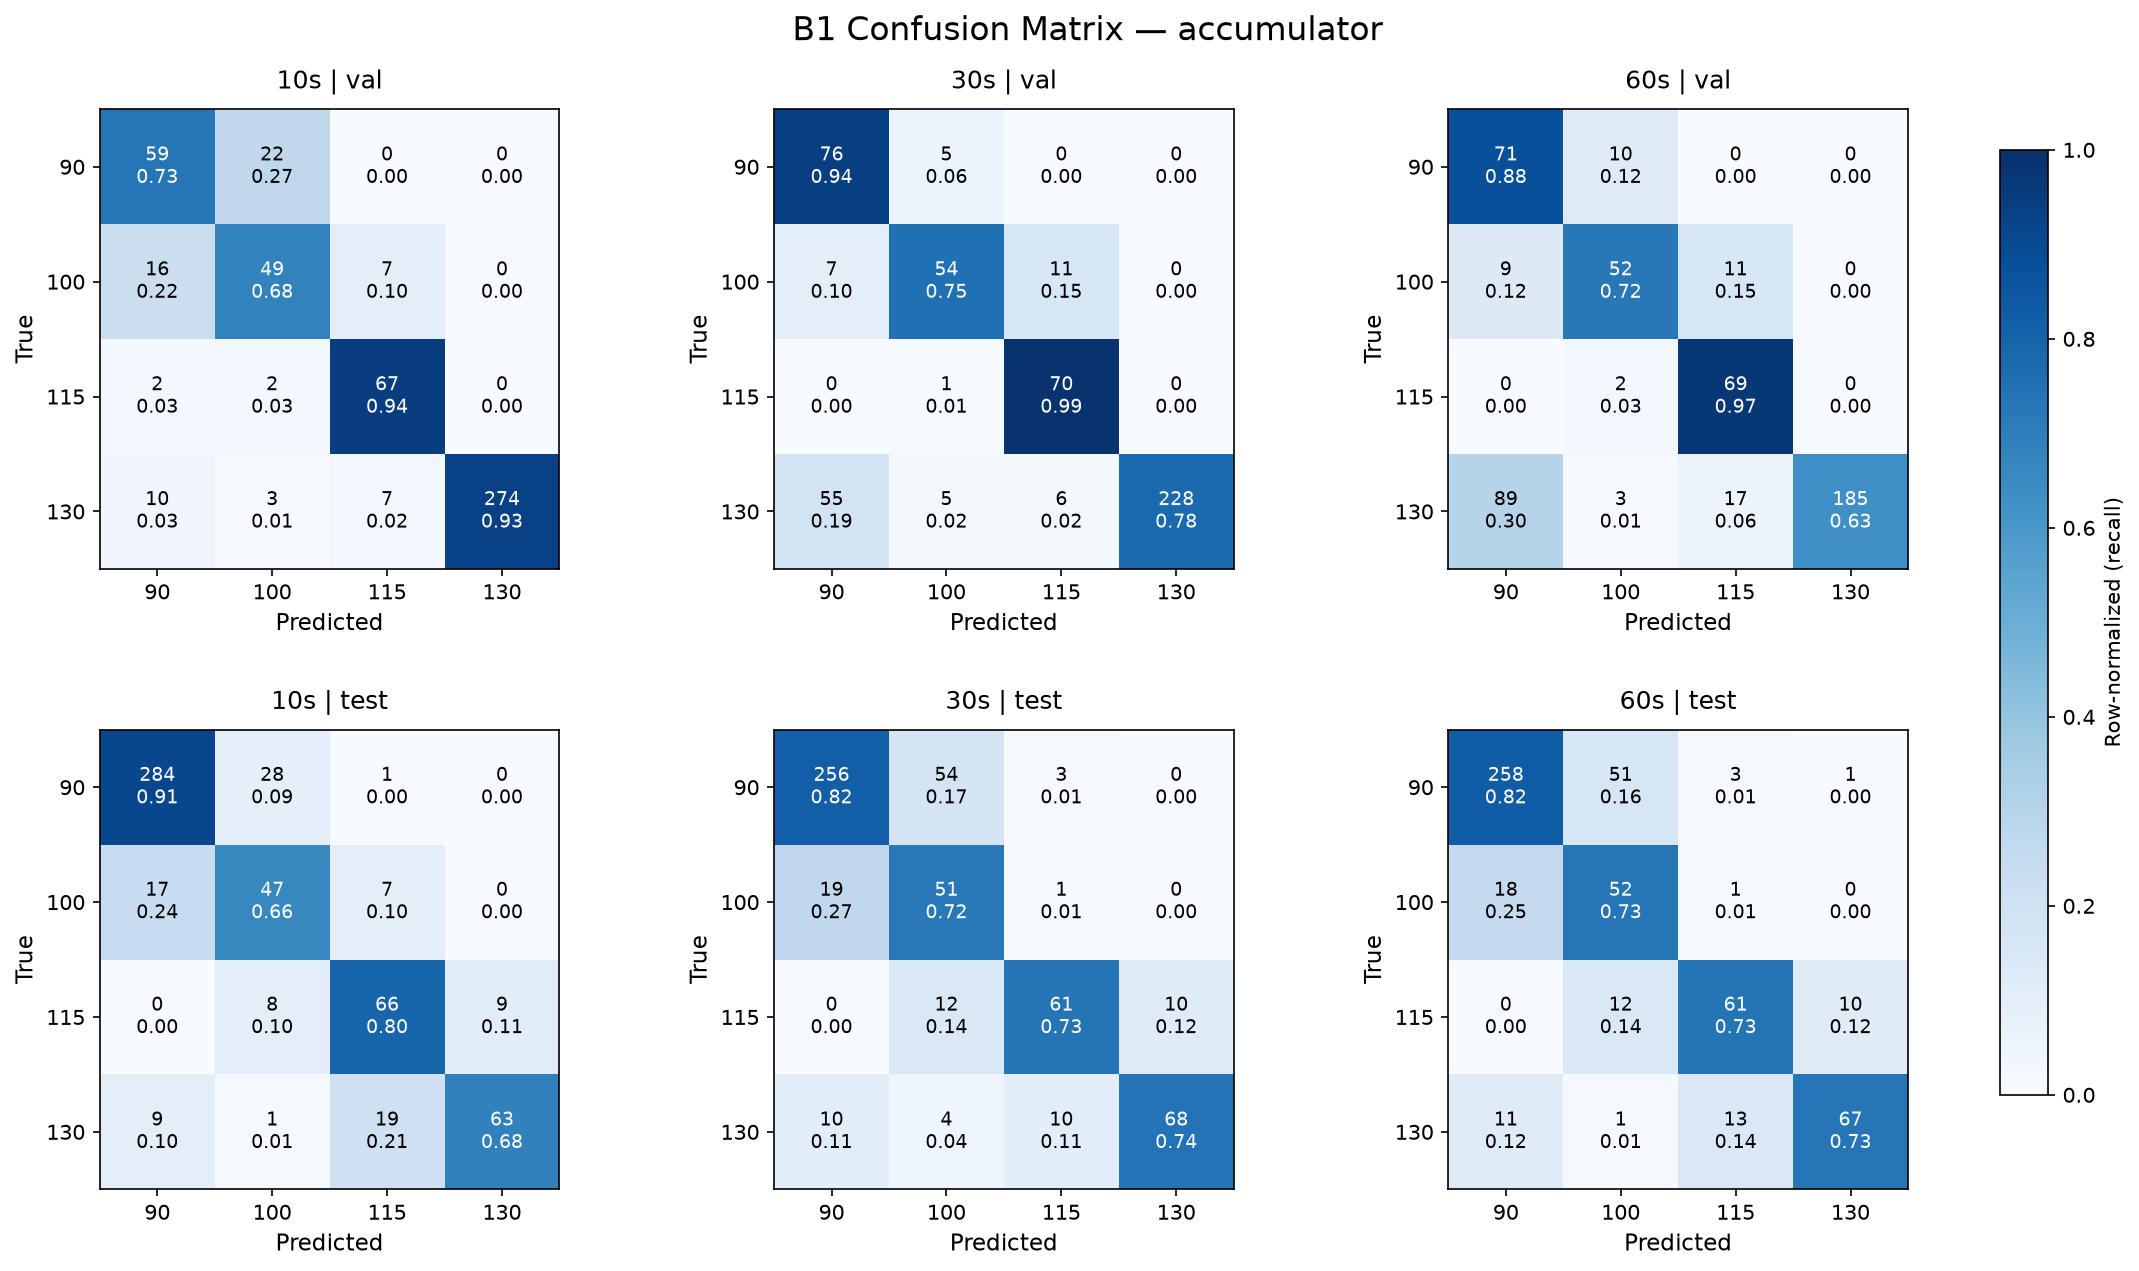
\includegraphics[width=\textwidth]{figures/cm_b1_accumulator.png}
        \caption{蓄能器部件混淆矩阵}
        \label{fig:cm_b1_accumulator}
    \end{subfigure}
    
    % 总标题与总标签
    \caption{引入分段统计与差分特征下四个液压部件的混淆矩阵对比}
    \label{fig:b1_all_confusion}
\end{figure}
对比召回率可知引入分段统计与差分特征的方案显著解决了基线B0模型在中等与较长观测窗口下阀门诊断性能严重退化的问题，全面提升了泵的诊断稳定性。阀门基线B0模型在30秒与60秒时间预算上Macro-F1仅为0.5-0.6区间，B1方案下达到0.88-0.97的高可用区间，证明了分段差分特征对捕捉动态过程故障的有效性。

泵部件B1方案在所有时间预算上均优于或者和基线B0方案持平。特别是在10秒短窗口下提升明显，从0.84进步至0.88，表明分段特征有助于在数据量较少时更敏感的捕捉瞬态异常。

冷却器部件中B1方案带来小幅提升，尤其是在较长时间预算下（30秒和60秒），说明对于稳态故障，增加趋势特征有一定的辅助作用，但是边际效应递减。

蓄能器提升有限，甚至在部分测试集略有波动，说明蓄能器的故障模式可能更依赖全局压力极值而非短期变化率。

总体而言，B1方案相对于B0的提升在于改进了平均化的缺陷，防止较长时间周期内抹平短期的故障信号，根据分段信息保留瞬态变化并使用差分标记放大变化较大的瞬间，同时增强短时窗口的信息密度，相当于从不同时间切片上多次观察信号，增加特征空间的维度，使得随机森林模型更加容易找到决策边界。
\subsection{物理交叉特征引入}
\subsubsection{具体实现方法}
该方案在引入分段统计与差分特征的基础上加入物理交叉特征。包括energy\_per\_flow，具体计算公式为$$E_{flow} =\frac{\bar{P}_{EPS1}}{\bar{Q}_{FS1} + \epsilon}$$，即为单位流量的能量或者压力，物理上对应系统的负载效率和阻力特征。temp\_diff，数学公式为$$\Delta T = \bar{T}_{TS1} - \bar{T}_{TS4}$$，目标是计算两种油箱温度之间的温差，反映系统的热平衡状态和冷却效率。在工业检测场景中引入领域知识构建特征可以有效的提升模型的可解释性和泛化能力。后文使用B3代指此方案。
\subsubsection{具体结果分析}
下图展示在引入分段统计与差分特征、物理交叉特征后四个部件的混淆矩阵示意图。该方案提升了部分组件的诊断鲁棒性，证明了物理交叉特征在机械故障诊断中的价值。

在泵部件上，B3是最佳的方案，在30秒和60秒下Macro-F1均超过0.96，且随着时间增加性能稳步提升，说明物理交叉特征有效捕捉泵的累积性故障特征。其原因在于泵是旋转机械，其故障常表现为压力和流量关系的非线性变化，B3引入的energy\_per\_flow直接关联了功率和流量，物理意义明确，泵的效率下降或者内泄会导致相同流量下压力变化或者相同压力下流量异常，使用比值模拟物理量乐意放大这种效率偏离，比均值或者标准差更具有判别力。

冷却器表现极其稳定，测试集上F1维持在0.99左右，验证了温度类故障的稳态特性，物理特征起到了辅助确认作用，温差提供了额外的冗余信息，增强了模型的鲁棒性。

阀门部件相比B1出现重大异常，虽然在10秒时间预算下表现完美（F1=1.0），但是在60秒时间预算下测试集F1下跌至0.6左右，说明B3引入的物理交叉特征或者分段策略在长窗口下引入噪声，或者未能正确刻画阀门在长周期内的动态滞后特性，导致模型过拟合短窗口的瞬态特征。

蓄能器部件表现平稳但无显著突破，测试集F1在0.74-0.75之间，说明当前特征体系对蓄能器故障的敏感度已经达到瓶颈。
\begin{figure}[H]
    \centering
    % 第一行两张子图
    \begin{subfigure}[b]{0.45\textwidth}
        \centering
        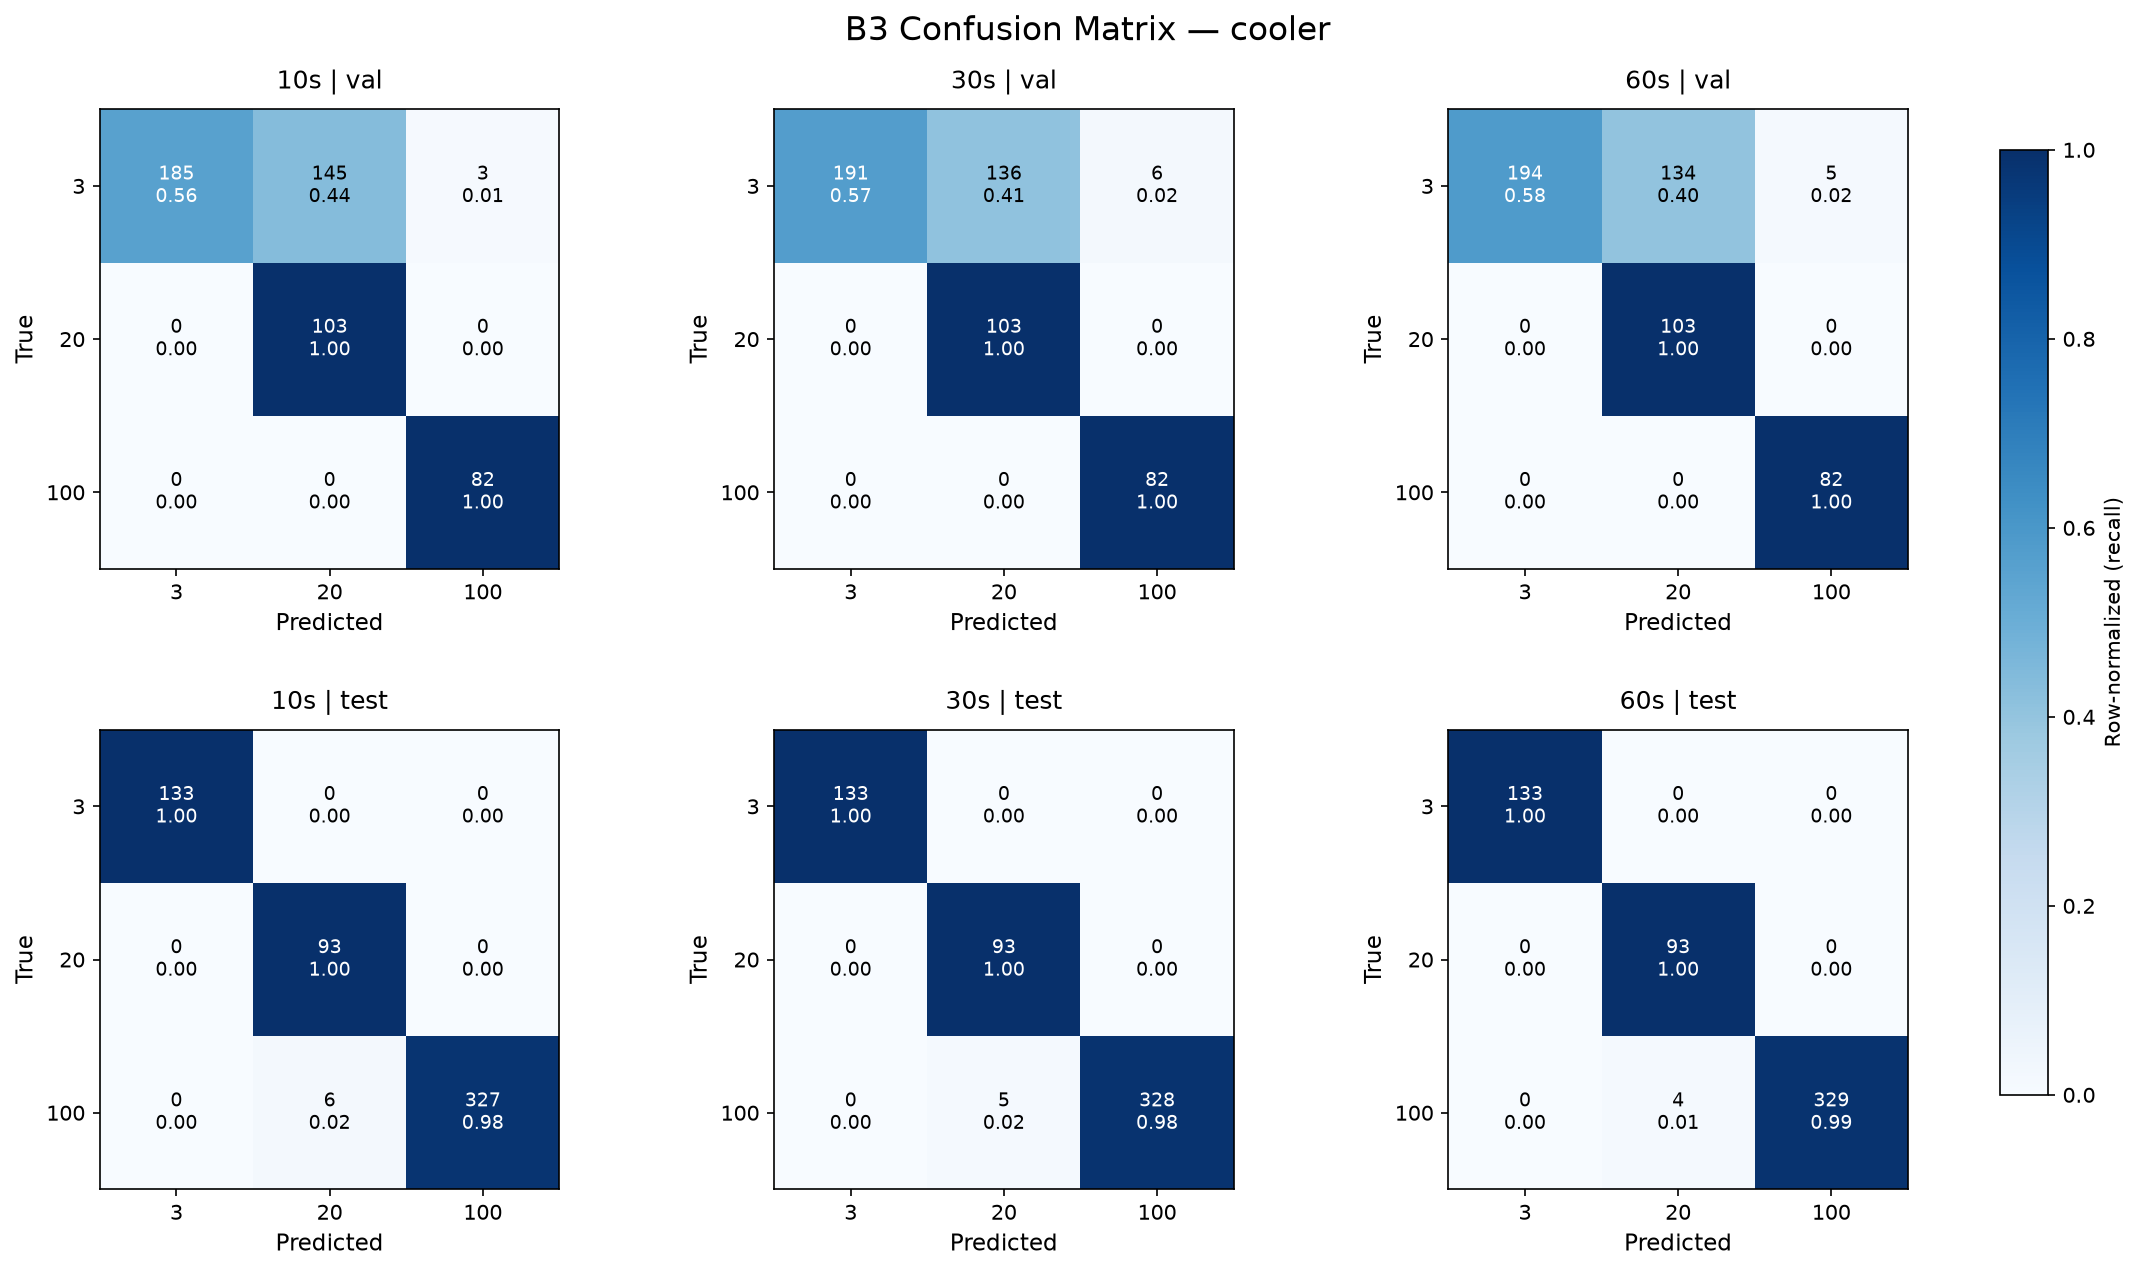
\includegraphics[width=\textwidth]{figures/cm_b3_cooler.png}
        \caption{冷却器部件混淆矩阵}
        \label{fig:cm_b3_cooler}
    \end{subfigure}
    \hfill
    \begin{subfigure}[b]{0.45\textwidth}
        \centering
        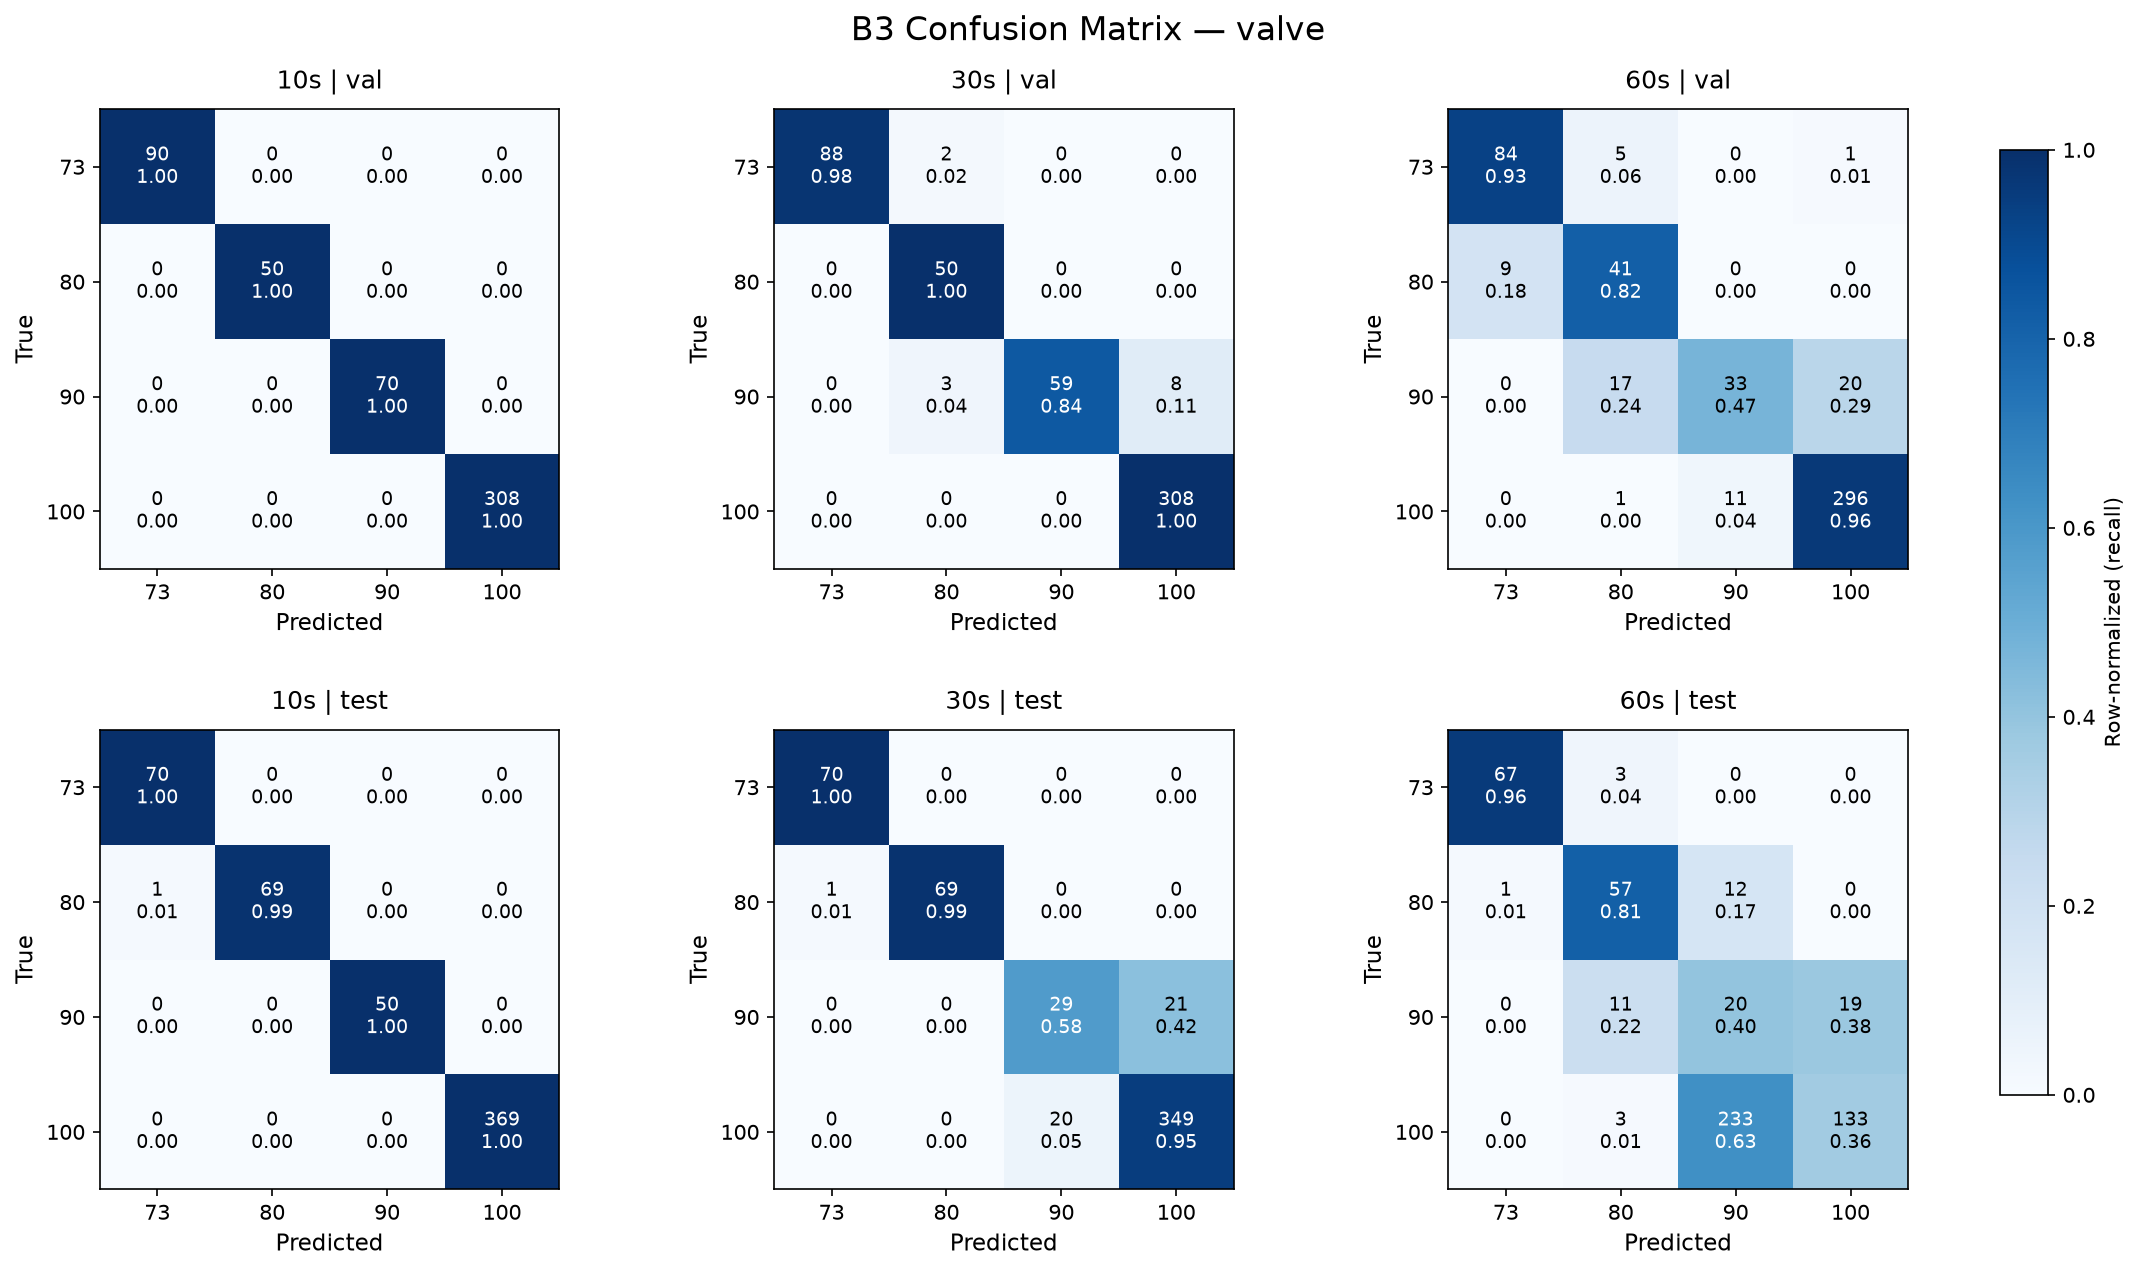
\includegraphics[width=\textwidth]{figures/cm_b3_valve.png}
        \caption{阀门部件混淆矩阵}
        \label{fig:cm_b3_valve}
    \end{subfigure}
    
    % 第二行两张子图
    \vspace{0.5cm}
    \begin{subfigure}[b]{0.45\textwidth}
        \centering
        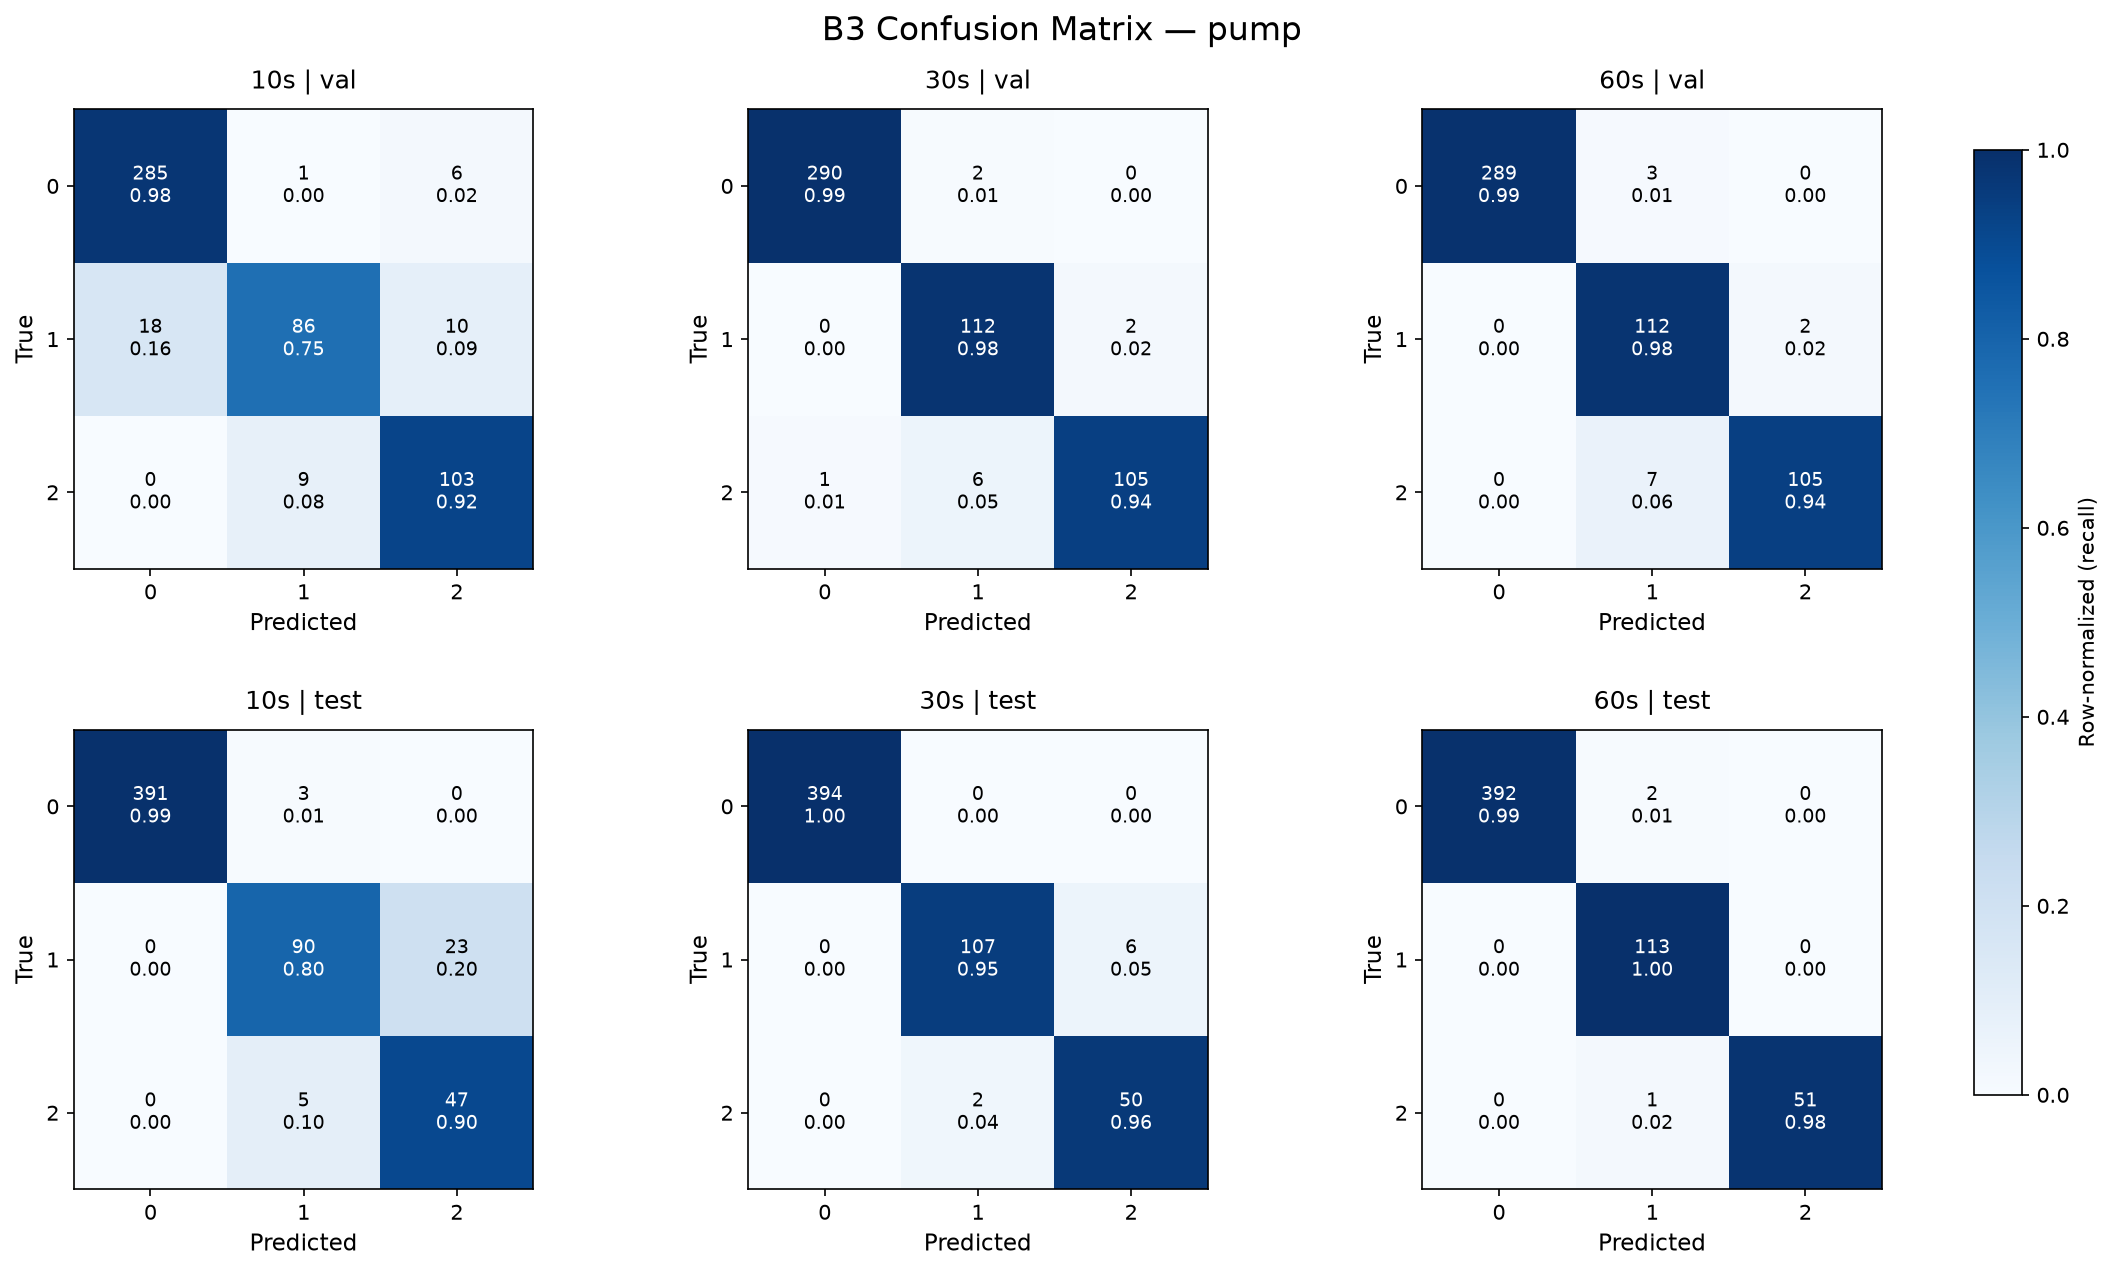
\includegraphics[width=\textwidth]{figures/cm_b3_pump.png}
        \caption{泵部件混淆矩阵}
        \label{fig:cm_b3_pump}
    \end{subfigure}
    \hfill
    \begin{subfigure}[b]{0.45\textwidth}
        \centering
        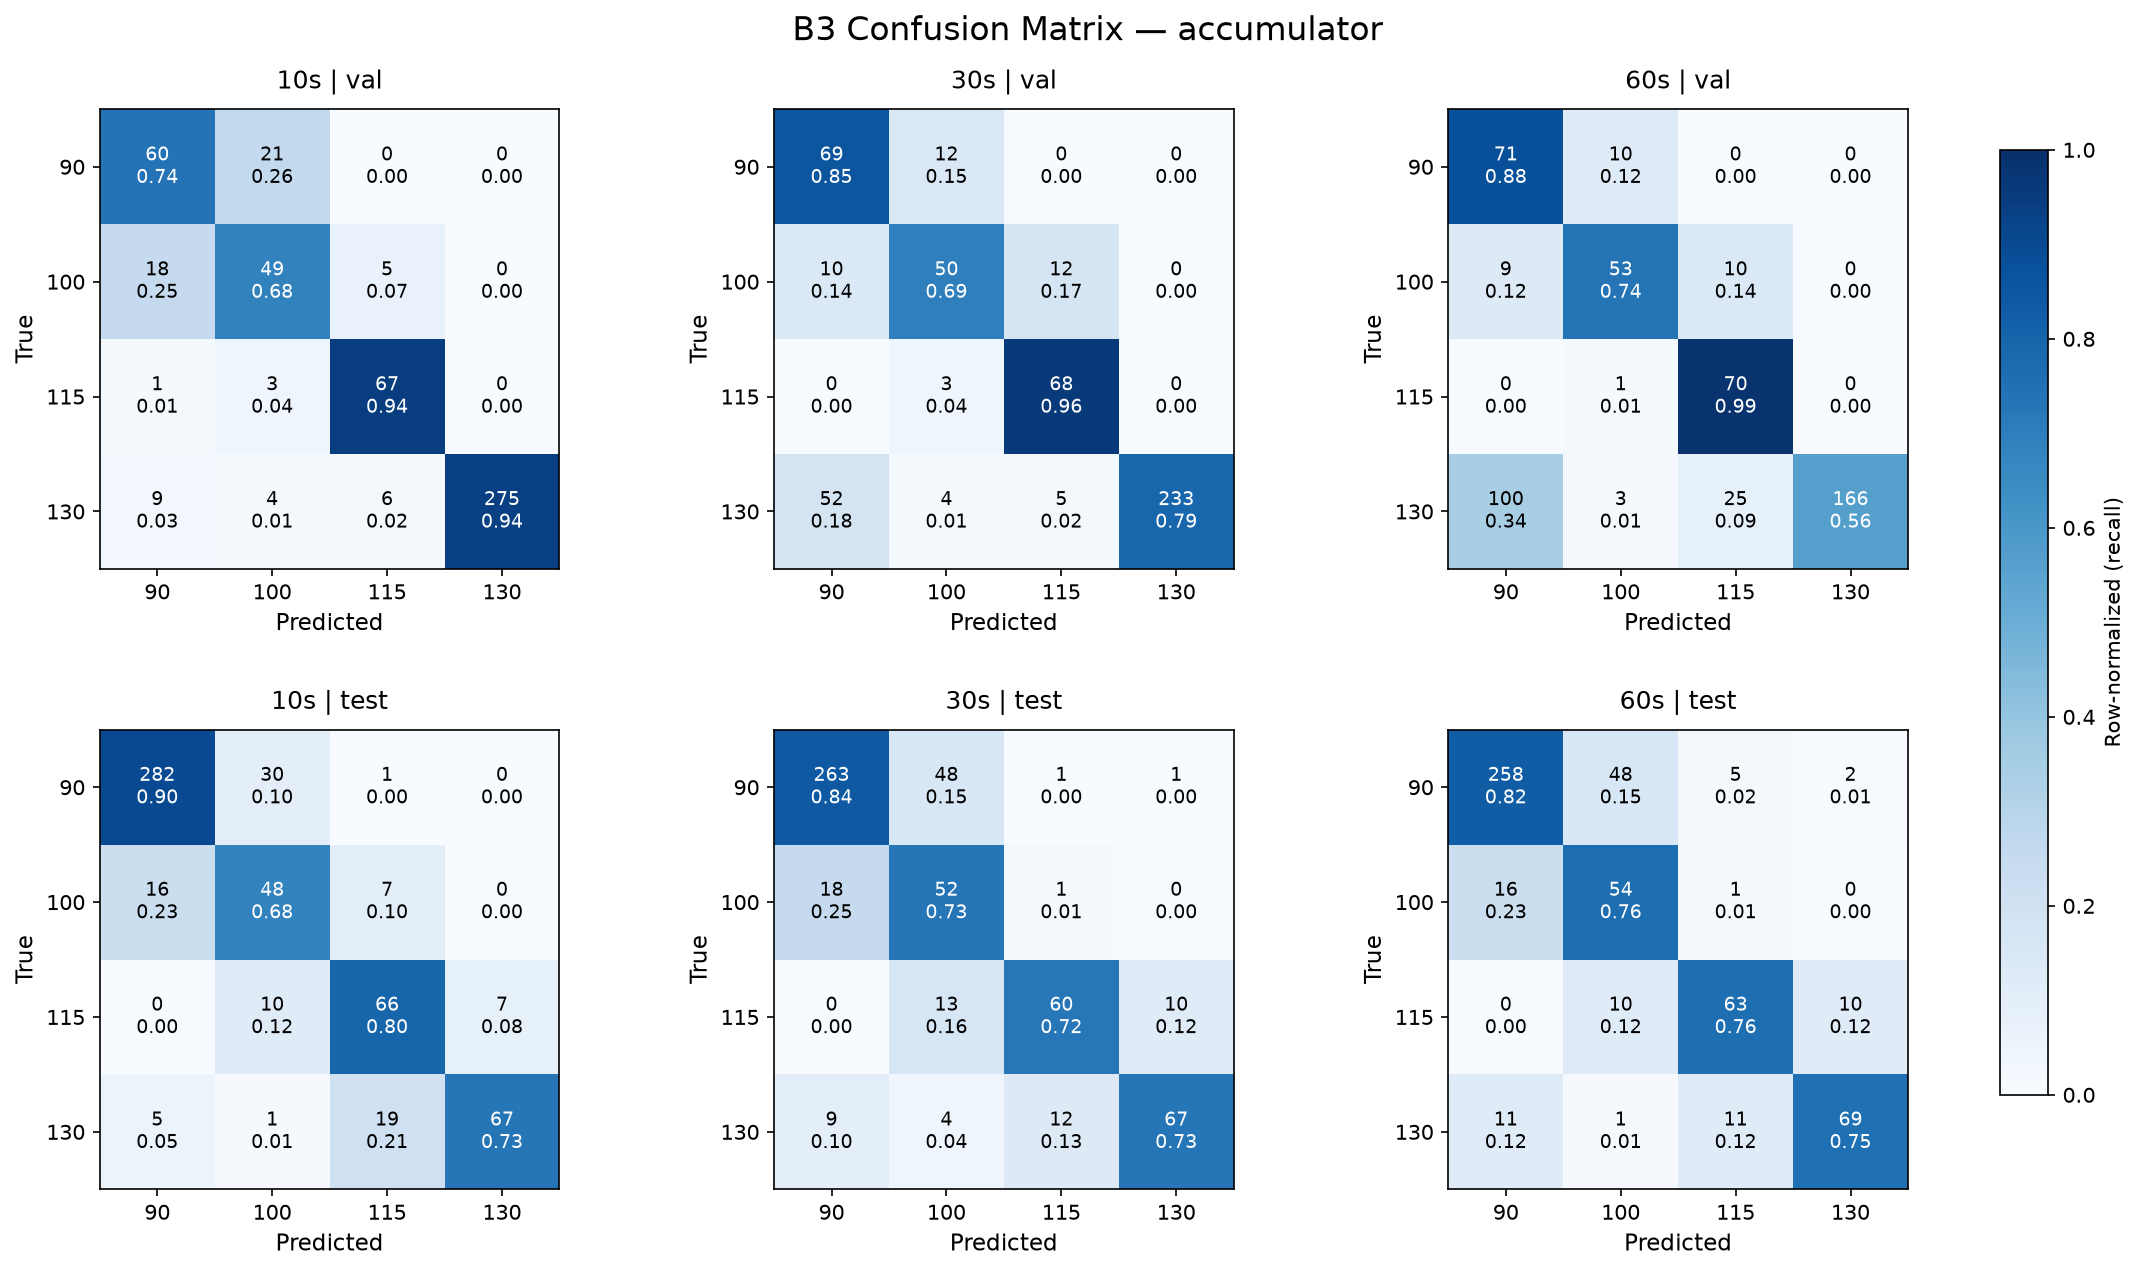
\includegraphics[width=\textwidth]{figures/cm_b3_accumulator.png}
        \caption{蓄能器部件混淆矩阵}
        \label{fig:cm_b3_accumulator}
    \end{subfigure}
    
    % 总标题与总标签
    \caption{引入分段统计差分特征物理交叉特征下四个液压部件的混淆矩阵对比}
    \label{fig:b3_all_confusion}
\end{figure}
\subsection{消融对比实验分析}
\subsubsection{差分特征消融验证}
方案B2目标为验证B1方案中引入的分段差分特征是否对模型性能有实质性贡献，是否是冗余特征或者引入了噪声。B2特征提取包含六种全局统计量和三个分段均值，移除两个差分特征，其他随机森林参数、缺失值处理、数据划分、观测预算条件完全保持一致。原假设为分段均值已经包含足够的时序信息，差分特征是冗余的，移除后性能不会显著下降，甚至可能因为减少噪声而提升。备择假设为差分特征捕捉了信号的非平稳变化，是诊断动态故障的关键，移除后性能将显著下降。

下图展示基于差分特征的消融实验四个部件的混淆矩阵示意图。

在泵部件上，B2的保留分段均值已经能够很好的刻画持续性偏移特征，在较长时间预算上Macro-F1已经接近1.0，分段均值充分平滑噪声，保留故障趋势。对于该部件而言差分特征是冗余的，B2证明仅靠分段均值即可实现高精度诊断，模型特征更为简洁。

冷却器部件不需要复杂的时序差分特征，全局统计量或者分段均值足以刻画，Macro-F1指标和B0以及B1几乎完全一致。

阀门部件展现出明显的因为差分特征缺失导致的失效问题，其故障具有强烈的瞬态和非平稳特性。B2方案在较长时间预算上的Macro-F1相对于B1出现明显下滑，关键原因在于信息丢失，对于分段均值可能包含大量稳态数据变得相似，模型难以区分正常与异常。差分特征直接量化了动作端和稳态段的落差，提供了重要的监督信号，移除差分后需要从两个高度相关的均值特征中学习落差，在长窗口噪声环境下非常困难。

对于蓄能器部件B2方案和B1出现波动较小，整体仍然处于瓶颈期，其故障可能更依赖频域特征或者极值统计，时域分段均值或差分对其帮助有限。

总体而言，B2实验成功验证了差分特征的价值，对于动态部件（如阀门）保留差分的方案B1在通用性上明显优于B2，有效的克服了长窗口平均化的问题。
\begin{figure}[H]
    \centering
    % 第一行两张子图
    \begin{subfigure}[b]{0.45\textwidth}
        \centering
        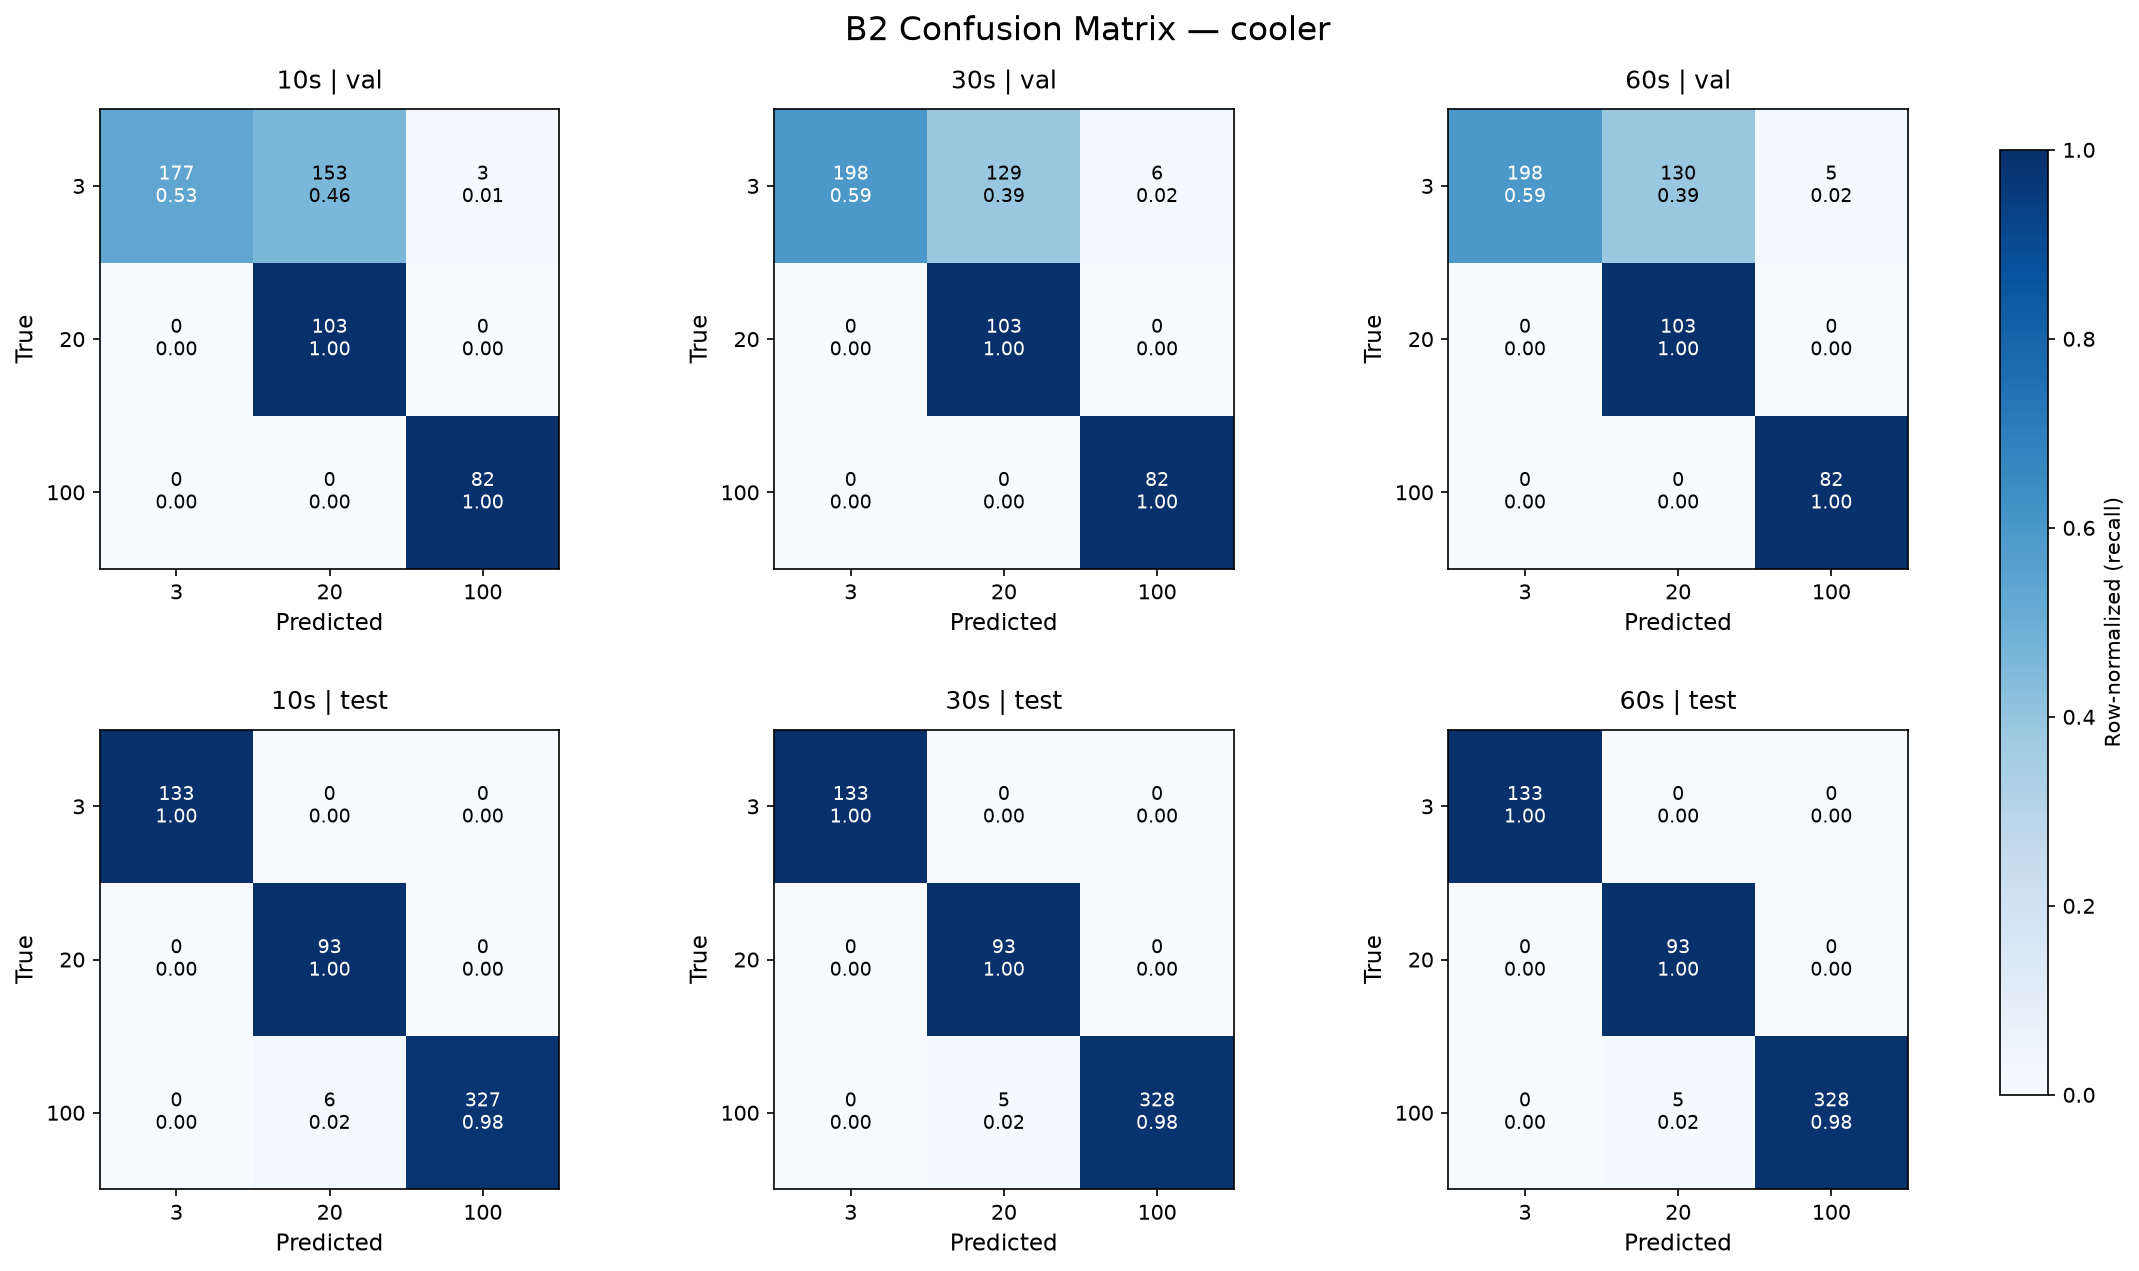
\includegraphics[width=\textwidth]{figures/cm_b2_cooler.png}
        \caption{冷却器部件混淆矩阵}
        \label{fig:cm_b2_cooler}
    \end{subfigure}
    \hfill
    \begin{subfigure}[b]{0.45\textwidth}
        \centering
        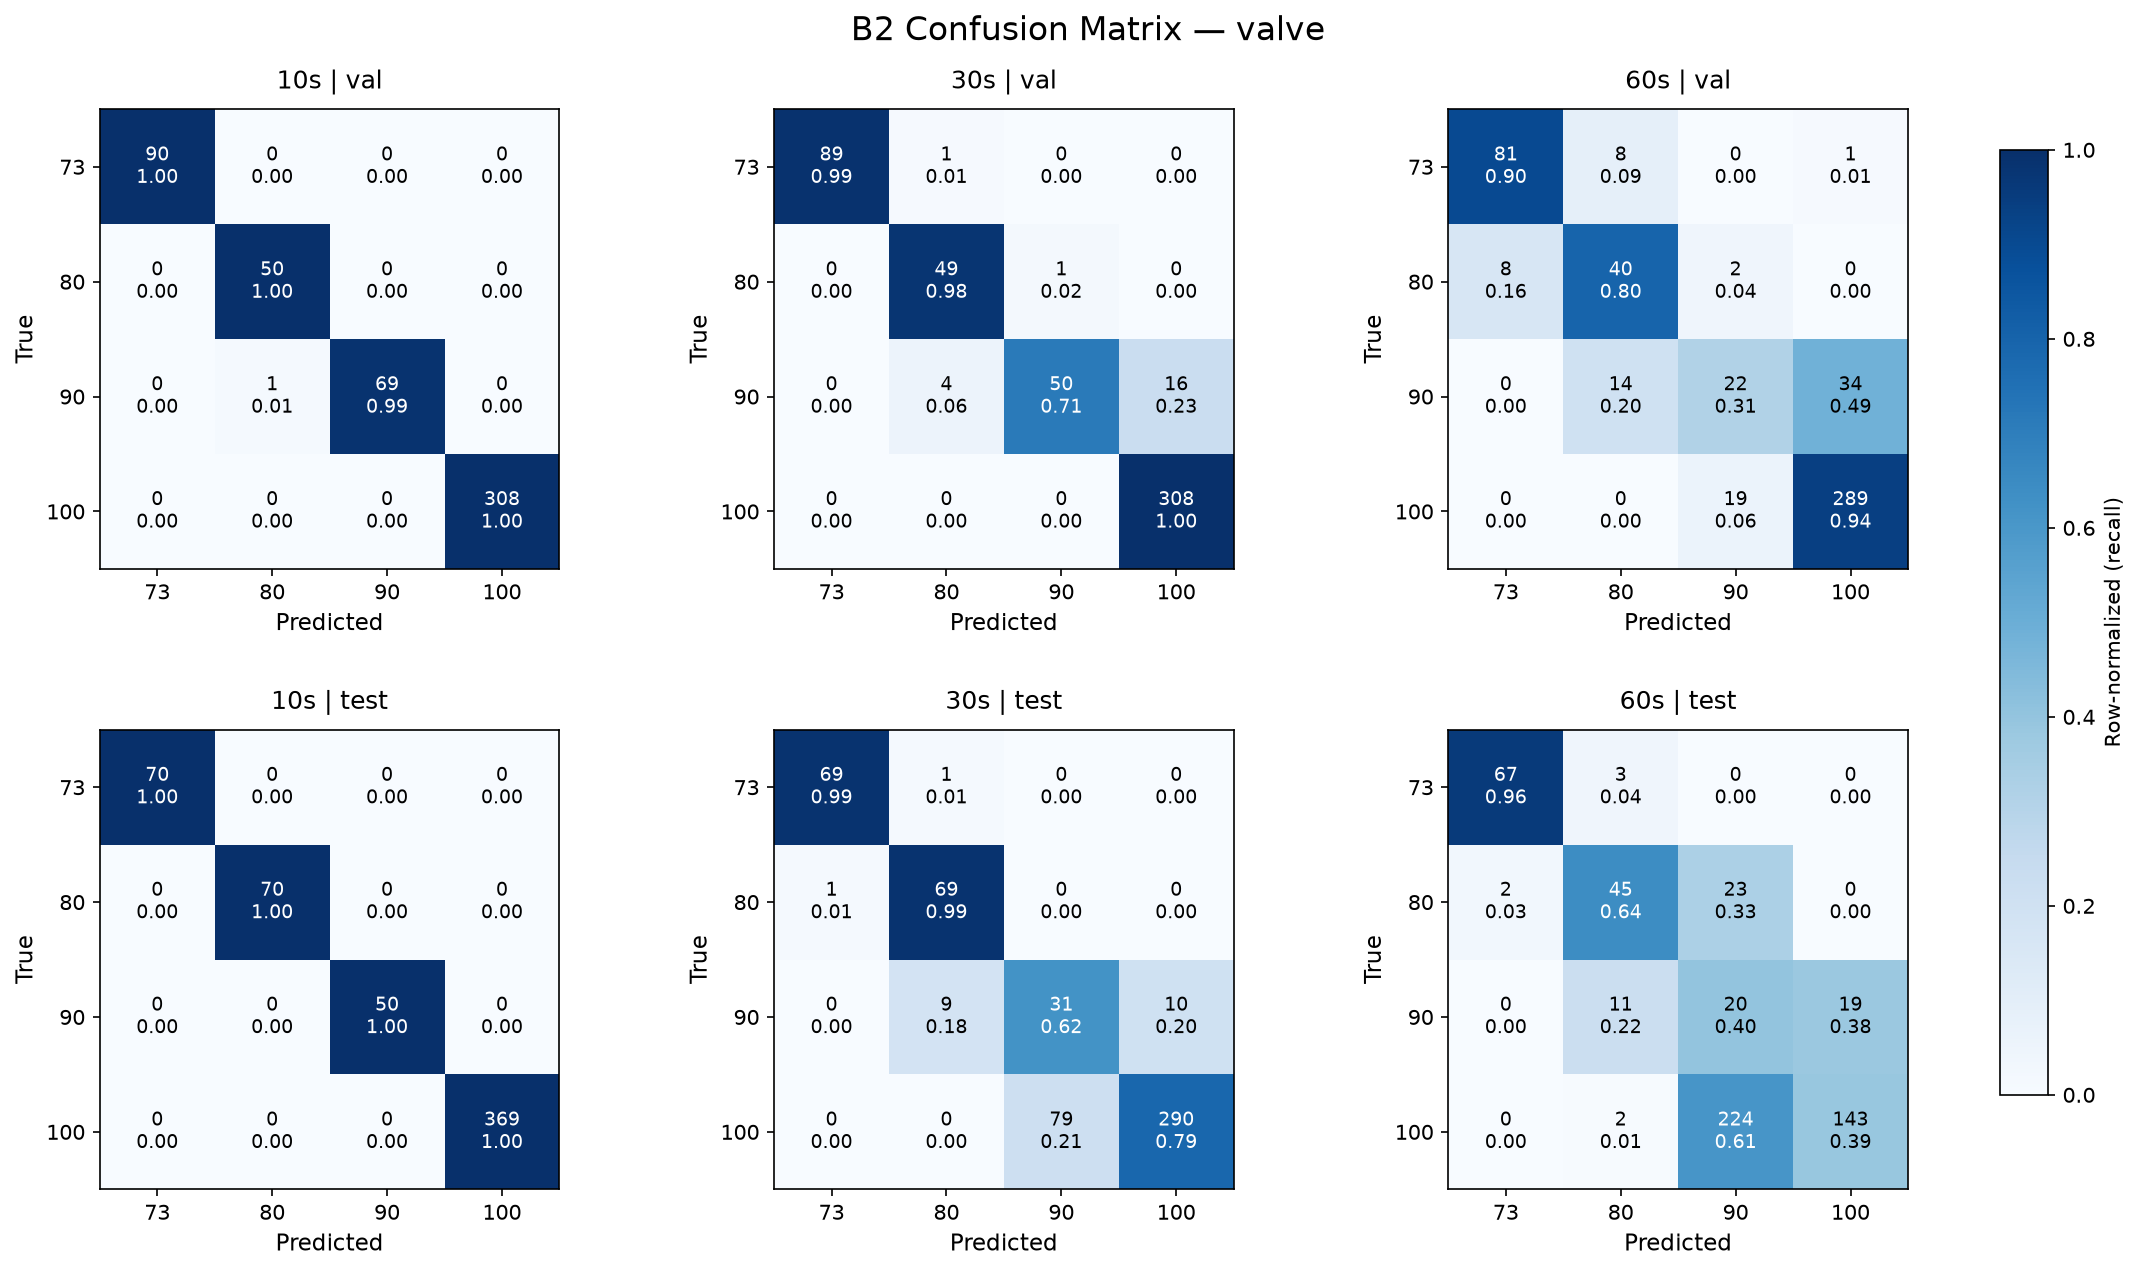
\includegraphics[width=\textwidth]{figures/cm_b2_valve.png}
        \caption{阀门部件混淆矩阵}
        \label{fig:cm_b2_valve}
    \end{subfigure}
    
    % 第二行两张子图
    \vspace{0.5cm}
    \begin{subfigure}[b]{0.45\textwidth}
        \centering
        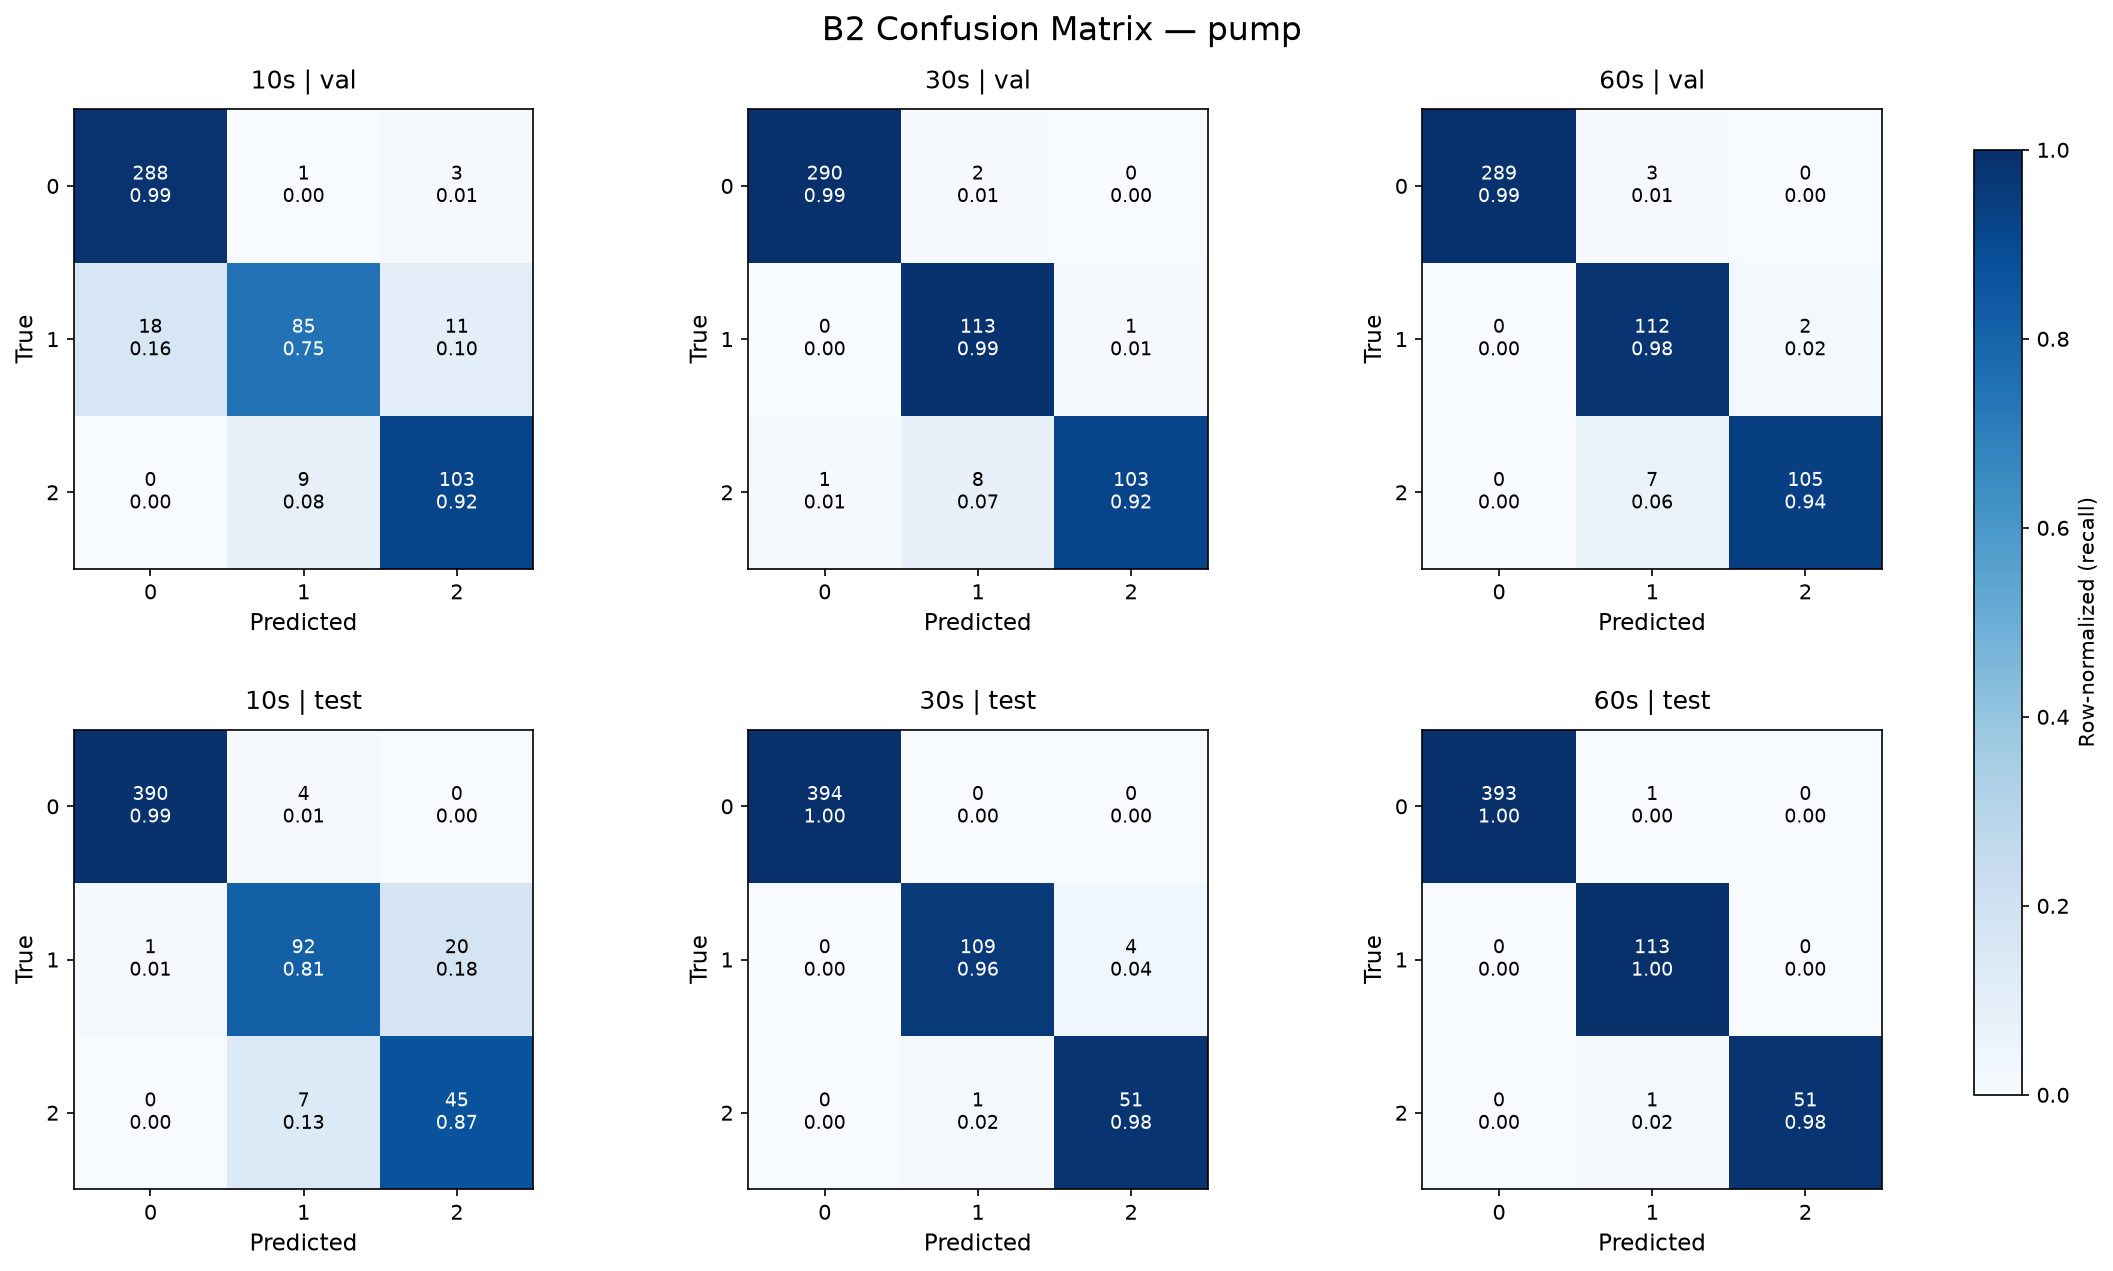
\includegraphics[width=\textwidth]{figures/cm_b2_pump.png}
        \caption{泵部件混淆矩阵}
        \label{fig:cm_b2_pump}
    \end{subfigure}
    \hfill
    \begin{subfigure}[b]{0.45\textwidth}
        \centering
        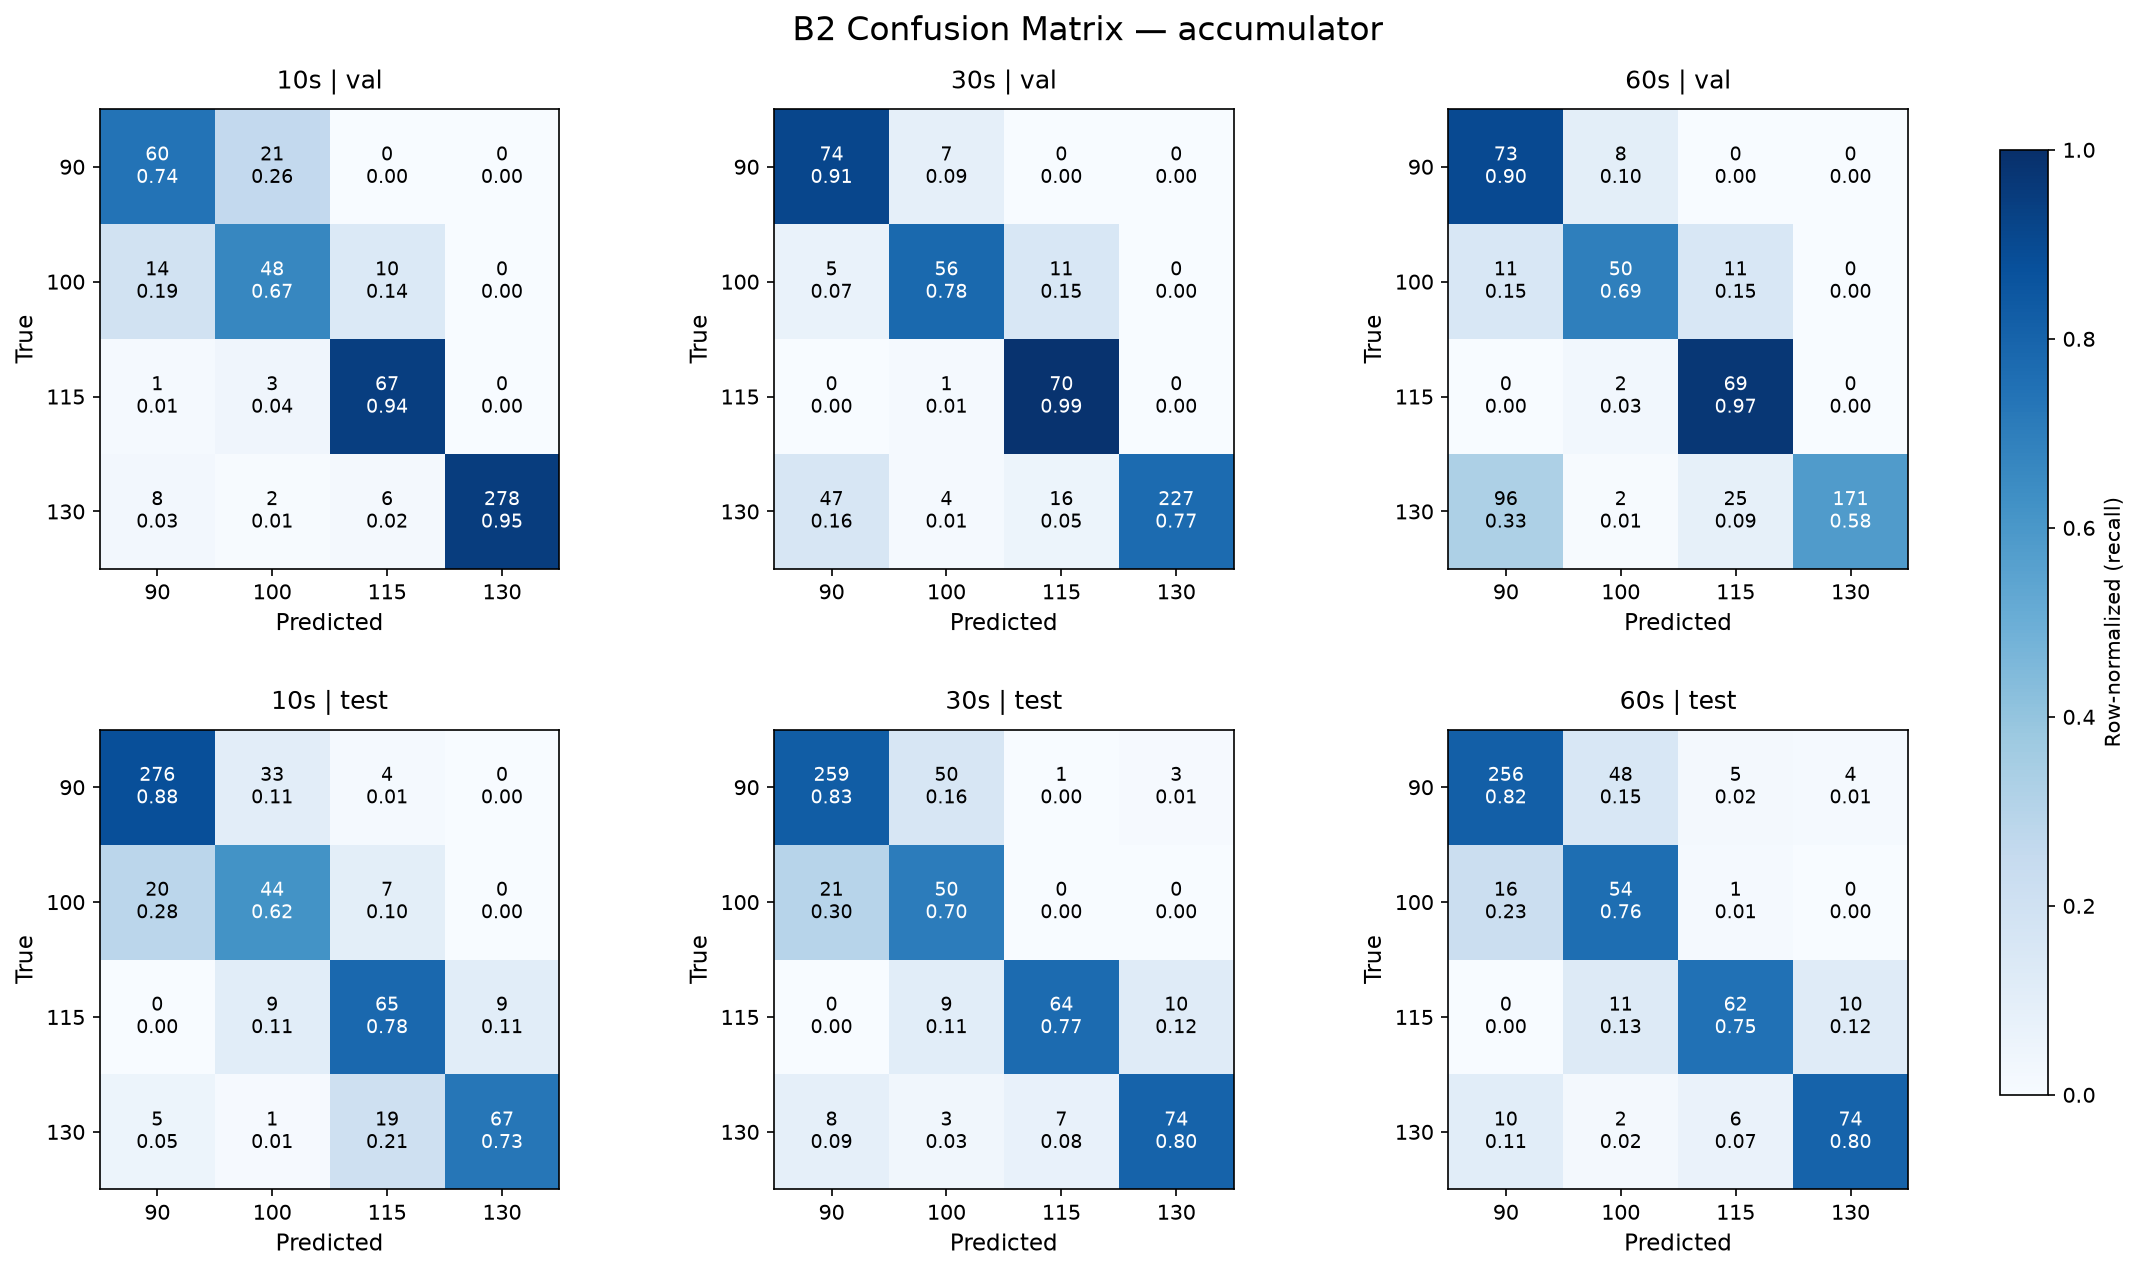
\includegraphics[width=\textwidth]{figures/cm_b2_accumulator.png}
        \caption{蓄能器部件混淆矩阵}
        \label{fig:cm_b2_accumulator}
    \end{subfigure}
    
    % 总标题与总标签
    \caption{引入分段统计与差分特征下四个液压部件的混淆矩阵对比}
    \label{fig:b2_all_confusion}
\end{figure}
\subsubsection{物理交叉特征消融验证}
方案B4进行交叉消融实验，核心设计逻辑是验证B3方案中引入的物理交叉特征在缺乏分段时序特征的情况下是否依然有效，确定物理机理和时序动态在故障诊断中的相对贡献。对于B0和B4，需要证明是否物理交叉特征具有强大的独立判别能力，在没有复杂的时序建模的情况下也可以因为领域知识显著提升效果。

下图展示在仅引入物理交叉特征后四个部件的混淆矩阵示意图。物理特征适用于反映系统整体能效或者稳态偏差的部件，不适用于反映瞬态响应特性的部件。

对于泵部件物理特征的加入表现优秀，而且显著优于未加入物理特征的短窗口表现，说明加入的物理特征有效的捕捉了泵的能效偏移。

对于冷却器部件B4表现稳定，测试集F1维持在0.99左右，温度差提供了直接的物理判据，弥补了单纯温度均值可能存在的工况漂移误差。

阀门部件出现严重失效，长时间预算严重低于短时间预算且低于其他方案。在没有分段差分的情况下，全局物理比值被长窗口的稳态数据稀释，无法捕捉阀门动作初期的异常。

蓄能器表现平稳，和其他方案差异不大，物理特征带来微弱增益，但是未能突破瓶颈。
\begin{figure}[H]
    \centering
    % 第一行两张子图
    \begin{subfigure}[b]{0.45\textwidth}
        \centering
        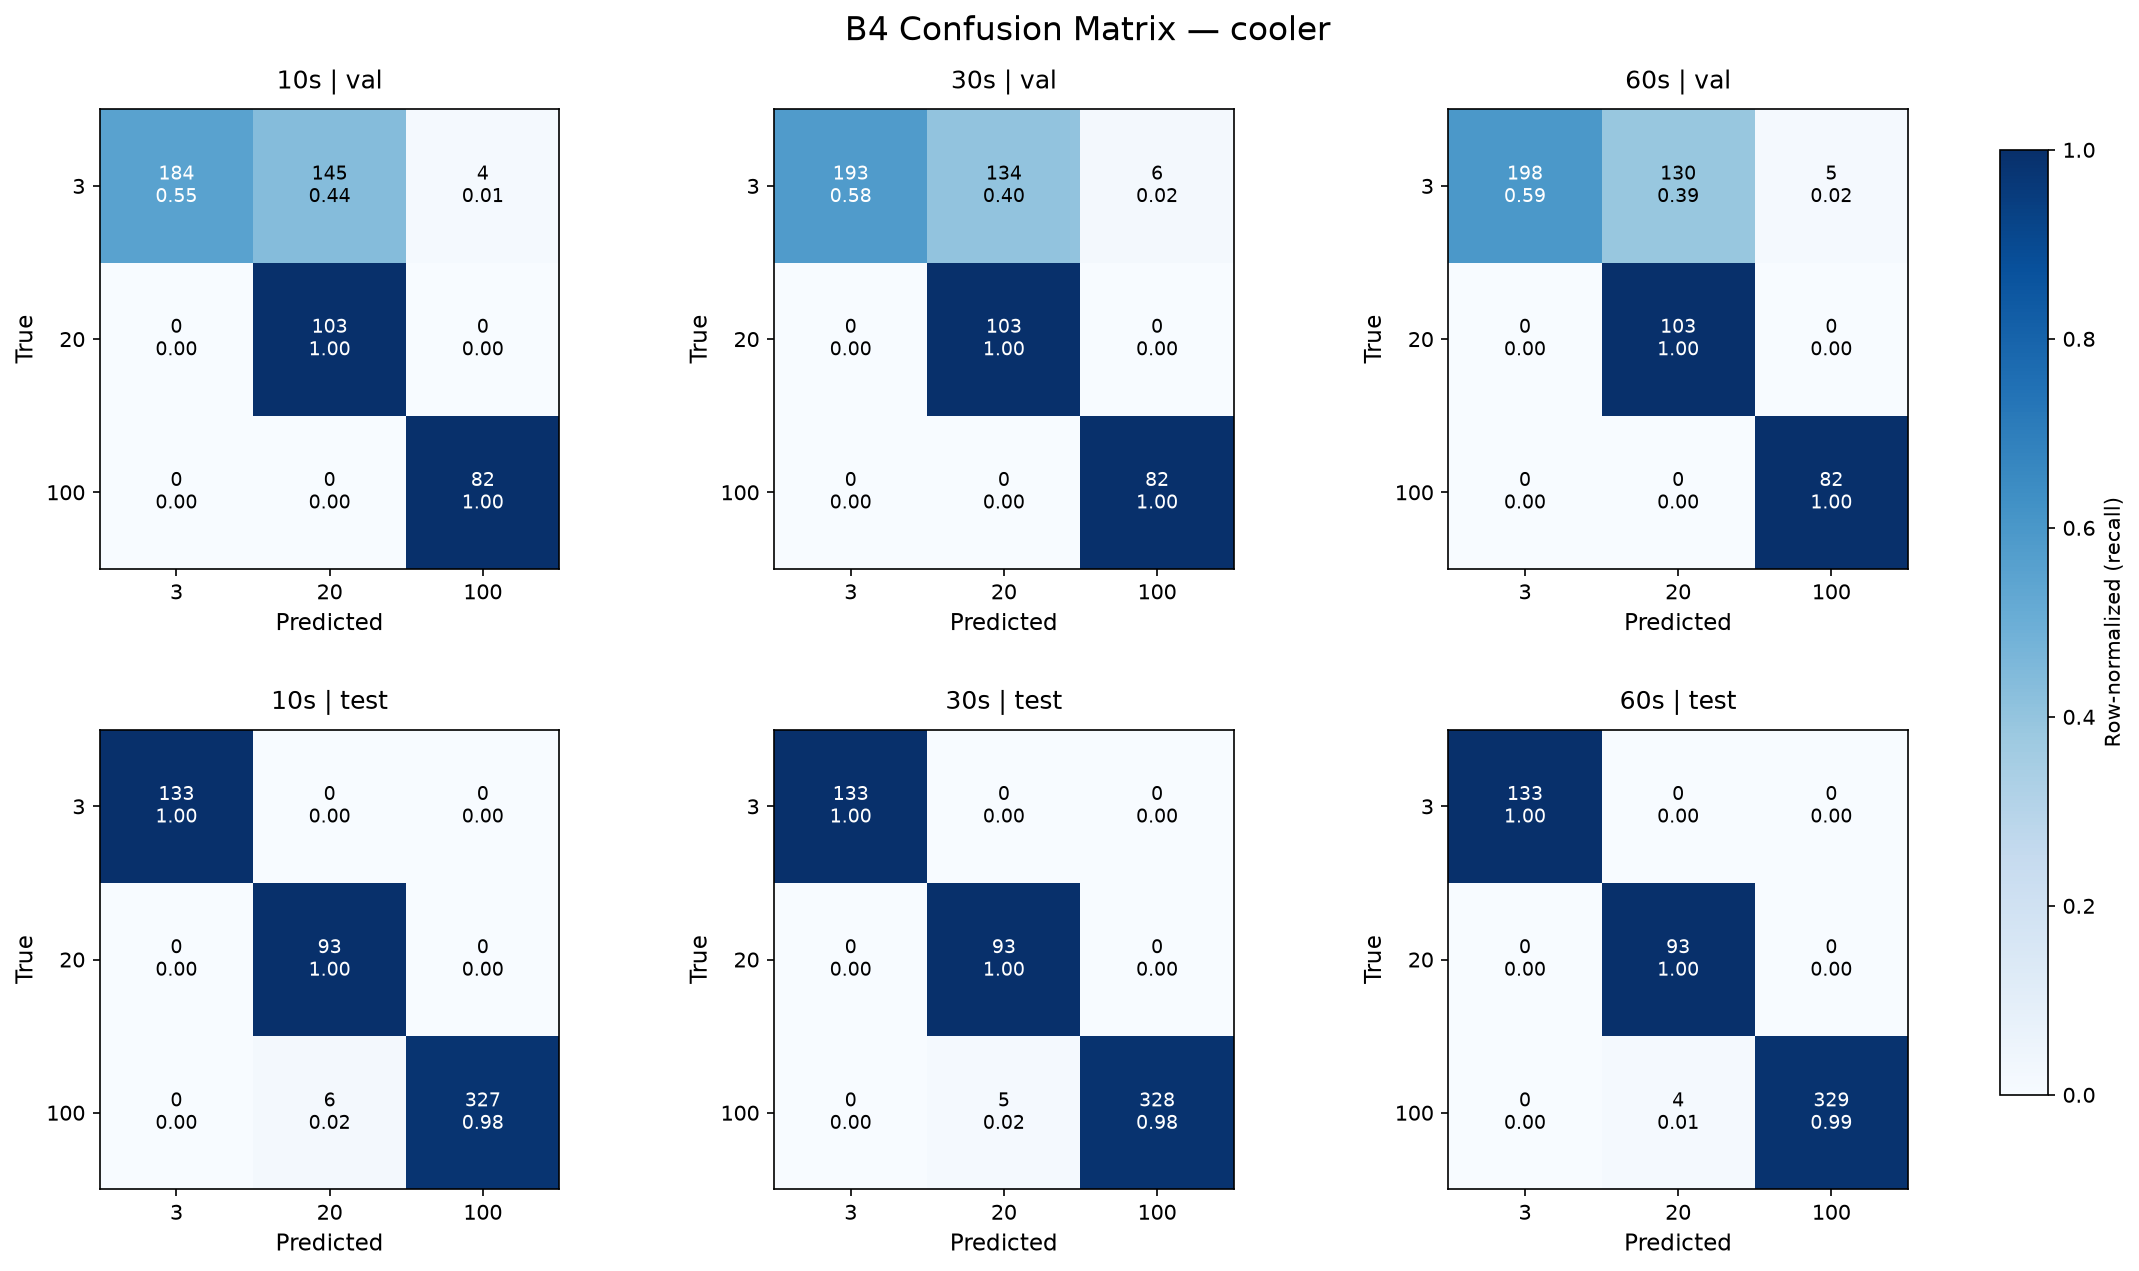
\includegraphics[width=\textwidth]{figures/cm_b4_cooler.png}
        \caption{冷却器部件混淆矩阵}
        \label{fig:cm_b4_cooler}
    \end{subfigure}
    \hfill
    \begin{subfigure}[b]{0.45\textwidth}
        \centering
        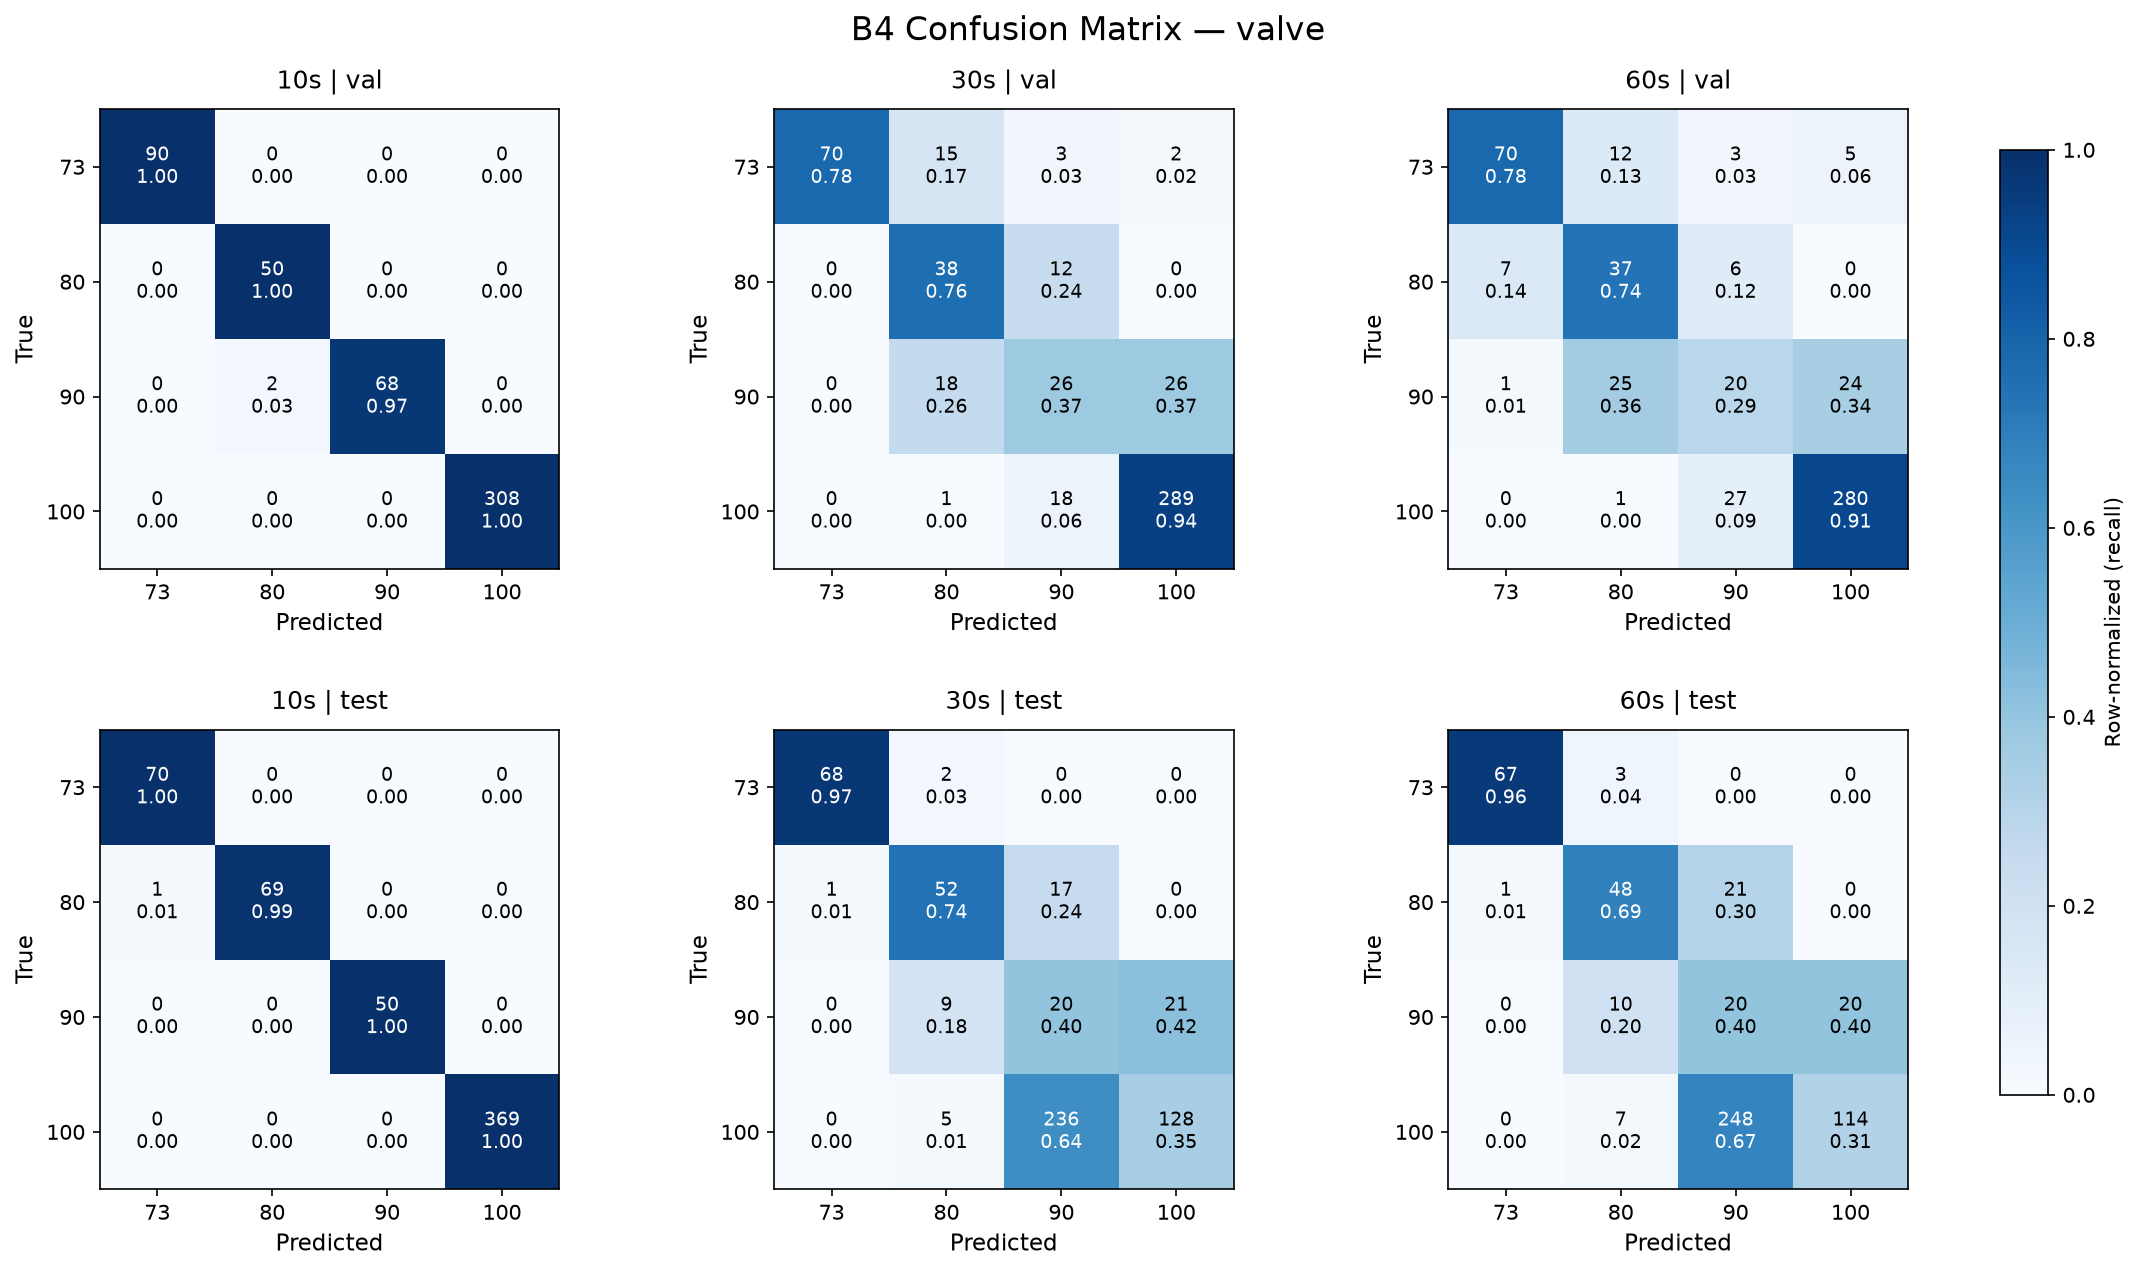
\includegraphics[width=\textwidth]{figures/cm_b4_valve.png}
        \caption{阀门部件混淆矩阵}
        \label{fig:cm_b4_valve}
    \end{subfigure}
    
    % 第二行两张子图
    \vspace{0.5cm}
    \begin{subfigure}[b]{0.45\textwidth}
        \centering
        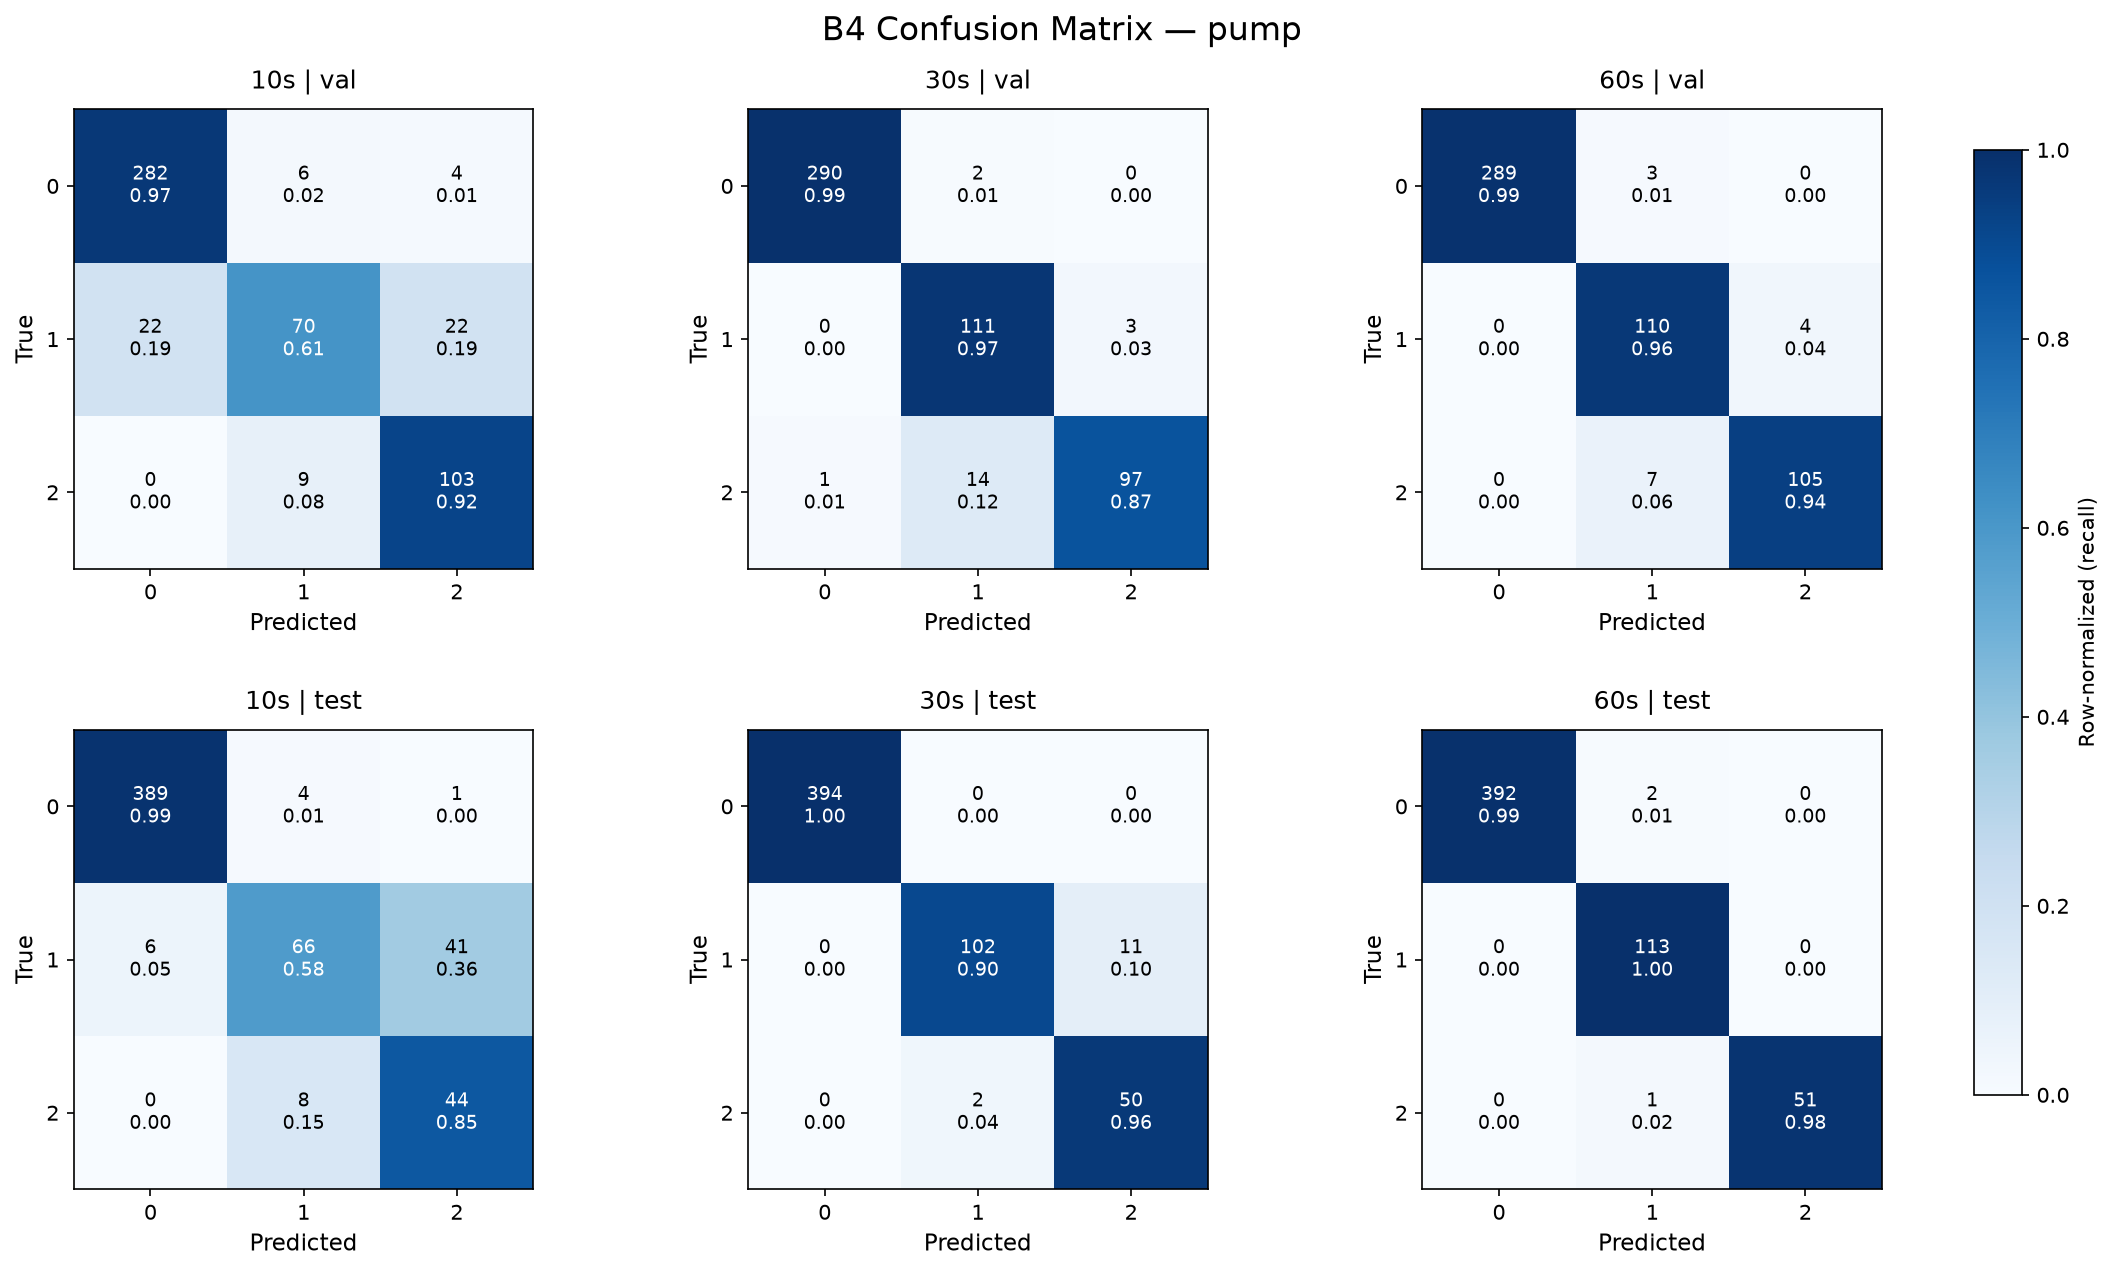
\includegraphics[width=\textwidth]{figures/cm_b4_pump.png}
        \caption{泵部件混淆矩阵}
        \label{fig:cm_b4_pump}
    \end{subfigure}
    \hfill
    \begin{subfigure}[b]{0.45\textwidth}
        \centering
        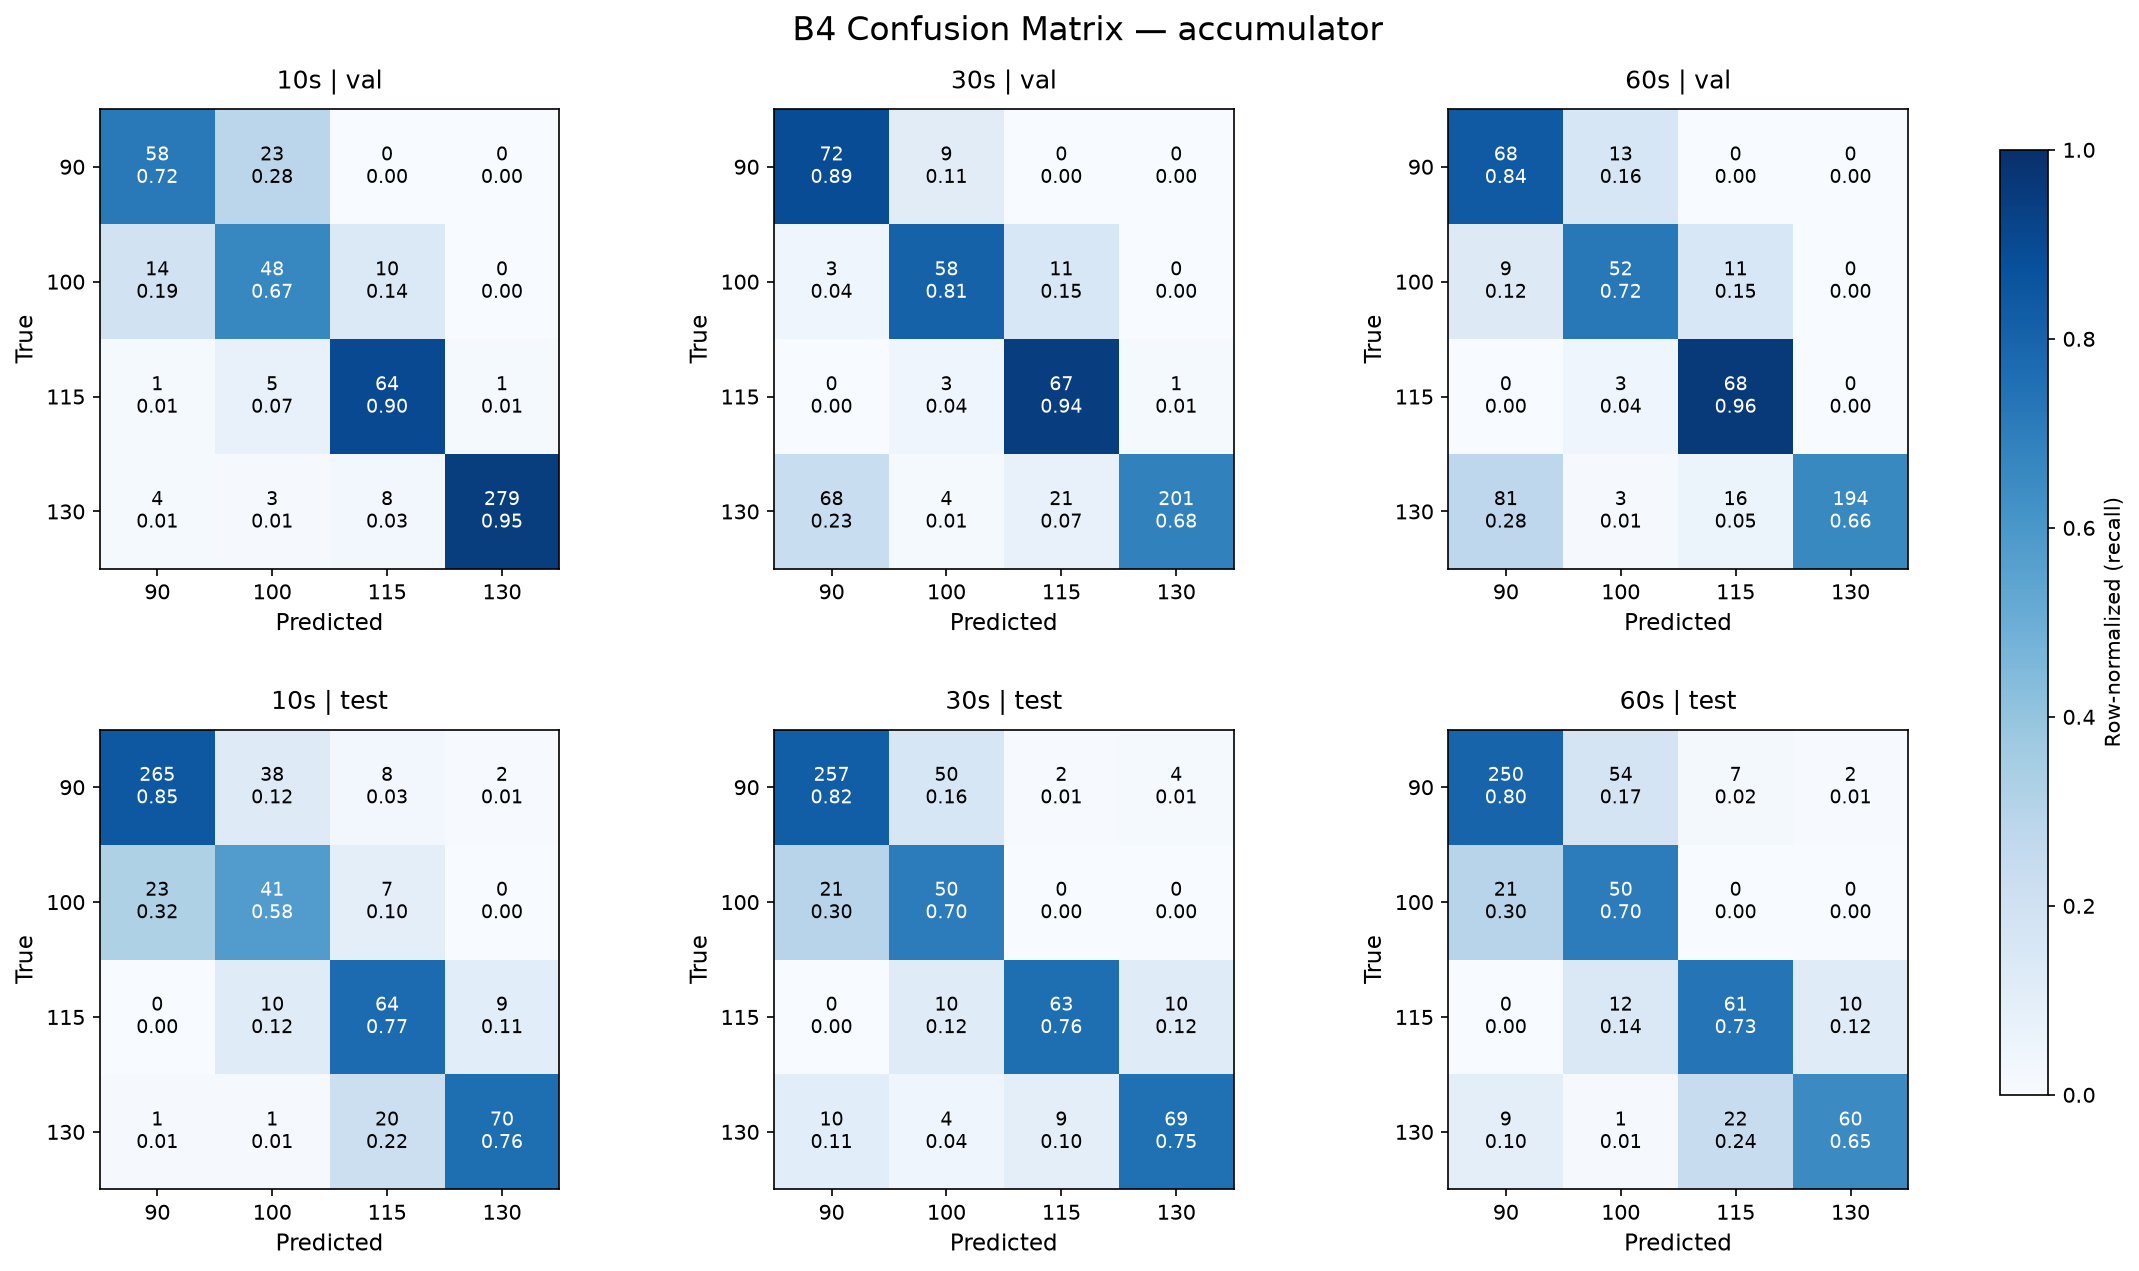
\includegraphics[width=\textwidth]{figures/cm_b4_accumulator.png}
        \caption{蓄能器部件混淆矩阵}
        \label{fig:cm_b4_accumulator}
    \end{subfigure}
    
    % 总标题与总标签
    \caption{引入分段统计与差分特征下四个液压部件的混淆矩阵对比}
    \label{fig:b4_all_confusion}
\end{figure}
\subsection{前缀时长与改进有效性的归因分析}
\subsubsection{10秒与60秒差别来源}
从 B1 的四个随机森林模型中读取特征重要性，并按所属通道聚合（四部件取平均），得到不同观测预算下的通道重要性对比如下表所示。短窗口与长窗口所依赖的信号存在明显差异：10秒时重要性最高的是 EPS1（0.152）、PS1（0.145）与 PS2（0.128），即电机功率与主/控制压力的瞬态极值和变化率；而到 60 秒时，FS1的重要性由0.075 跃升至0.199成为第一主导通道，EPS1与PS1分别降至0.101 与0.080。其原因是：短窗口内阀切换、负载突变等瞬态事件尚未被平均，压力、功率的极值与斜率具有很强的判别力；窗口拉长到60秒后，这些瞬态被稳态均值稀释，模型转而依赖随时间持续存在的流量与温度信号（FS1 反映泵内泄漏流量，TS1--TS4反映热平衡状态）。这也解释了为何10秒的联合准确率普遍高于60秒。对性能瓶颈部件阀门而言，PS2控制压力在所有预算下都是最重要的通道（0.28--0.42），说明阀门的切换滞后主要体现在控制压力的亚秒级瞬态上，与错误案例分析中的结论一致。

\begin{table}[H]
  \centering
  \caption{各通道特征重要性按观测预算对比（B1，四部件取平均）}
  \label{tab:feat_imp_budget}
  \small
  \begin{tabular}{lccc}
    \toprule
    \textbf{通道} & \textbf{10 秒} & \textbf{30 秒} & \textbf{60 秒} \\
    \midrule
    FS1  & 0.0753 & 0.2098 & 0.1989 \\
    EPS1 & 0.1522 & 0.1109 & 0.1005 \\
    PS2  & 0.1277 & 0.0944 & 0.0988 \\
    TS4  & 0.0728 & 0.0845 & 0.0884 \\
    PS1  & 0.1454 & 0.0696 & 0.0796 \\
    PS3  & 0.0598 & 0.0911 & 0.0716 \\
    TS1  & 0.0466 & 0.0547 & 0.0580 \\
    PS5  & 0.0701 & 0.0520 & 0.0579 \\
    TS2  & 0.0495 & 0.0532 & 0.0574 \\
    FS2  & 0.0592 & 0.0477 & 0.0519 \\
    PS6  & 0.0722 & 0.0501 & 0.0516 \\
    TS3  & 0.0303 & 0.0426 & 0.0479 \\
    VS1  & 0.0256 & 0.0323 & 0.0286 \\
    PS4  & 0.0132 & 0.0072 & 0.0089 \\
    \bottomrule
  \end{tabular}
\end{table}

\subsubsection{改进对各个状态组合有效程度分析}
将测试集周期按四元组组合（冷却器\_阀\_泵\_蓄能器）聚合，比较B1与B0的联合准确率差值，结果如下两张表格所示。从逐部件整体增益看，改进几乎全部作用于阀门：阀门平均正确率提升0.106，而冷却器（+0.002）、泵（-0.002）基本不变，蓄能器仅+0.018。从组合层面看，增益最大的组合为3\_80\_0\_100（+0.700）、3\_80\_2\_100（+0.400）、100\_80\_1\_130（+0.300）——全部包含阀门异常；按是否含阀门异常分组，含阀门异常组合的最大增益为0.700，远高于不含阀门异常的0.238。这表明分段统计与差分特征的价值主要体现在阀门这类具有瞬态、非平稳切换行为的部件，而并非对所有部件、所有组合都普遍提升。

同时存在少量退化组合，如100\_73\_1\_130（-0.100）与20\_73\_1\_100（-0.100），均为含阀门异常的相邻等级组合，说明新增的分段差分特征在个别阀门边界样本上引入了额外波动。综合而言，改进具有明确的部件与组合选择性，其收益集中在阀门异常组合，未观察到对全部四部件的全局性提升。

\begin{table}[H]
  \centering
  \caption{B1相对B0的逐部件平均增益（60秒，全部测试周期）}
  \label{tab:improve_by_comp}
  \small
  \begin{tabular}{lccc}
    \toprule
    \textbf{部件} & \textbf{B0 正确率} & \textbf{B1 正确率} & \textbf{增益 $\Delta$} \\
    \midrule
    冷却器 & 0.991 & 0.993 & $+$0.002 \\
    阀门   & 0.420 & 0.526 & $+$0.106 \\
    泵     & 0.998 & 0.996 & $-$0.002 \\
    蓄能器 & 0.766 & 0.784 & $+$0.018 \\
    \bottomrule
  \end{tabular}
\end{table}

\begin{table}[H]
  \centering
  \caption{联合准确率增益最大与出现退化的状态组合（60秒，组合格式：冷却器\_阀\_泵\_蓄能器）}
  \label{tab:improve_by_group}
  \small
  \begin{tabular}{lcccc}
    \toprule
    \textbf{组合} & \textbf{周期数} & \textbf{B0 联合准确率} & \textbf{B1 联合准确率} & \textbf{$\Delta$} \\
    \midrule
    3\_80\_0\_100    & 10 & 0.300 & 1.000 & $+$0.700 \\
    3\_80\_2\_100    & 10 & 0.200 & 0.600 & $+$0.400 \\
    100\_80\_1\_130  & 10 & 0.700 & 1.000 & $+$0.300 \\
    100\_100\_0\_130 & 21 & 0.000 & 0.238 & $+$0.238 \\
    3\_100\_0\_90    & 21 & 0.238 & 0.476 & $+$0.238 \\
    3\_80\_2\_90     & 10 & 0.600 & 0.800 & $+$0.200 \\
    \midrule
    100\_100\_0\_115 & 21 & 0.619 & 0.571 & $-$0.048 \\
    100\_73\_1\_130  & 10 & 1.000 & 0.900 & $-$0.100 \\
    20\_73\_1\_100   & 10 & 0.300 & 0.200 & $-$0.100 \\
    \bottomrule
  \end{tabular}
\end{table}

\section{鲁棒性实验}
\subsection{实验设计和参数设置}
鲁棒性测试脚本使用evaluate\_robustness.py实现，目标在于在原始干净数据上主动注入故障扰动，模拟设备实际运行中可能遇到的5种典型异常，统一评测所有模型的性能衰减程度，量化不同特征方案的抗干扰能力。

测试条件包含如下5种：clean无任何扰动，使用原始数据，作为基准对照，验证所有模型在理想状态下的基线性能，和之前的训练结果做对齐校验。noise\_0.05给所有通道注入 0.05倍训练集标准差的高斯白噪声，模拟传感器长期使用后出现的电子漂移、现场电磁干扰、信号传输线路轻微抖动等常见噪声。noise\_0.10给所有通道注入 0.10倍训练集标准差的高斯白噪声，模拟恶劣工况下的强干扰。其中高斯噪声使用np.random.normal函数加入。掩码FS1把流量传感器FS1的全部数据置为NaN，模拟单个关键传感器完全失效，验证模型在缺失核心物理量时的容错能力。掩码FS1和FS2把两个流量传感器FS1、FS2全部置为NaN，模拟极端故障场景。

噪声生成时使用标准差完全来自训练集的统计量，防止使用测试集分布生成噪声造成的数据泄露问题，设定固定随机种子保证每次运行生成的噪声完全一致，实验结果可以复现。缺失值补偿使用训练阶段保存的中位数进行填充，不在测试阶段重新计算统计量，对于物理较差特征的计算完全基于被扰动之后的数据。
\subsection{鲁棒性验证结果分析}
下图展示60秒主结果下四部件对于不同工况噪声的鲁棒性折线统计图。下列表格展示详细指标数值。

针对鲁棒性测试的测试结果反映出方案B2综合性能最佳，在噪声场景下表现出最强的抗干扰能力。B1与B3在阀门动态故障诊断上保留了优势，但差分特征对于噪声更为敏感。B4的物理交叉特征在短窗口下抗噪性最差，所有方案在FS1传感器屏蔽场景下泵的诊断性能都出现严重下降，证明了泵的故障诊断对流量传感器的强物理依赖。

对于加入高斯噪声的场景而言。抗噪性排名B2优于B0优于B3优于B1优于B4，在0.1倍强噪声下，泵的60秒Macro-F1依然保持0.9868，几乎和干净数据持平。因为B2的核心特征是分段均值，均值运算天然具备低通滤波效果，能有效平滑高斯噪声，同时保留分段带来的时序信息，是兼顾性能和鲁棒性的最优解。B1和B3因为保留了差分特征，差分运算本质是高通滤波，会放大高频噪声，导致差分特征的数值出现剧烈抖动。但得益于长窗口下的大量样本平均，最终性能衰减幅度仍然控制在较小幅度，依然远优于B0的基线表现。在10秒短窗口下，泵的Macro-F1从干净数据的0.7716下降到0.5145。因为短窗口下样本点极少，噪声对均值的扰动被放大，直接导致energy\_per\_flow这个物理比值出现严重的数值漂移，完全失去了物理意义,证明基于全局均值的物理交叉特征，在短窗口下对噪声极其脆弱，必须搭配长窗口的平均化才能稳定工作‌。冷却器在所有噪声场景下性能几乎没有变化，因为温度信号本身变化极慢，噪声对均值的影响可以完全忽略；阀门在30秒窗口下的性能衰减幅度远小于60秒，因为短窗口下动作瞬态的信号能量远大于噪声能量。

对于传感器屏蔽场景而言，所有方案都具有物理依赖软肋。泵的性能全面严重下降，所有方案在FS1被屏蔽后，60秒窗口下泵的Macro-F1从接近1.0跌到0.13~0.58区间，失去流量传感器FS1的数据后，所有和流量相关的统计特征、物理交叉特征全部失效，仅靠压力信号无法区分正常流量漂移和故障内泄。其中B3与B4的性能最差，因为其核心物理特征energy\_per\_flow直接依赖FS1，即使经过中位数补偿也完全失去了物理判别力。阀门与冷却器几乎不受影响‌：阀门的诊断主要依赖压力和振动信号，冷却器完全依赖温度信号，FS1与FS2的屏蔽几乎不会干扰它们的特征提取，在所有传感器失效场景下，这两个部件的诊断性能和干净数据几乎完全一致。与此同时，B0在FS1屏蔽场景下泵的性能优于其他所有方案，原因是B0没有引入物理交叉特征，仅靠压力通道的统计特征，在中位数补偿后还能保留部分故障判别能力。其他方案引入的大量依赖FS1的特征在补偿后变成了无意义的常量，干扰模型的决策边界。
\begin{figure}[H]
    \centering
    % 第一行两张子图
    \begin{subfigure}[b]{0.45\textwidth}
        \centering
        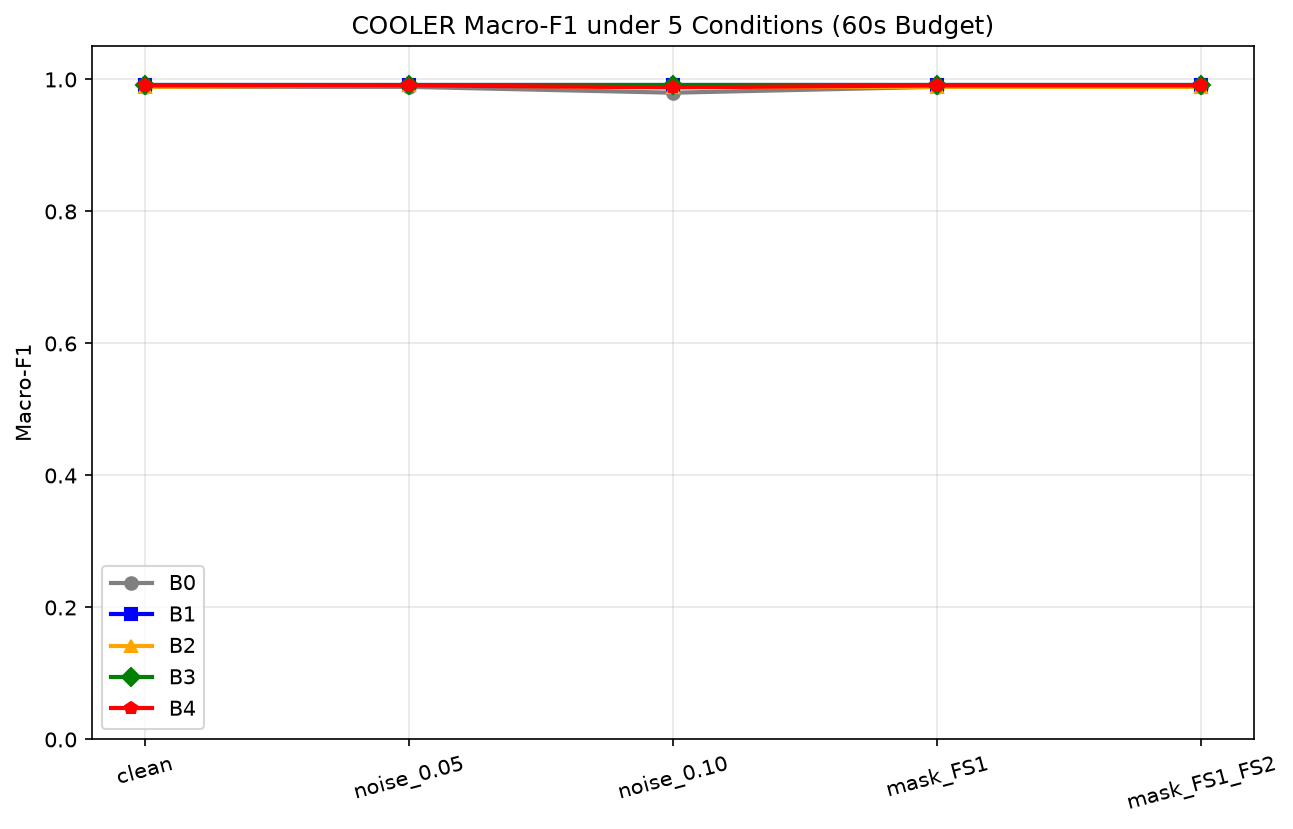
\includegraphics[width=\textwidth]{figures/robustness_cooler_60s.png}
        \caption{冷却器部件鲁棒性比较}
        \label{fig:robustness_cooler}
    \end{subfigure}
    \hfill
    \begin{subfigure}[b]{0.45\textwidth}
        \centering
        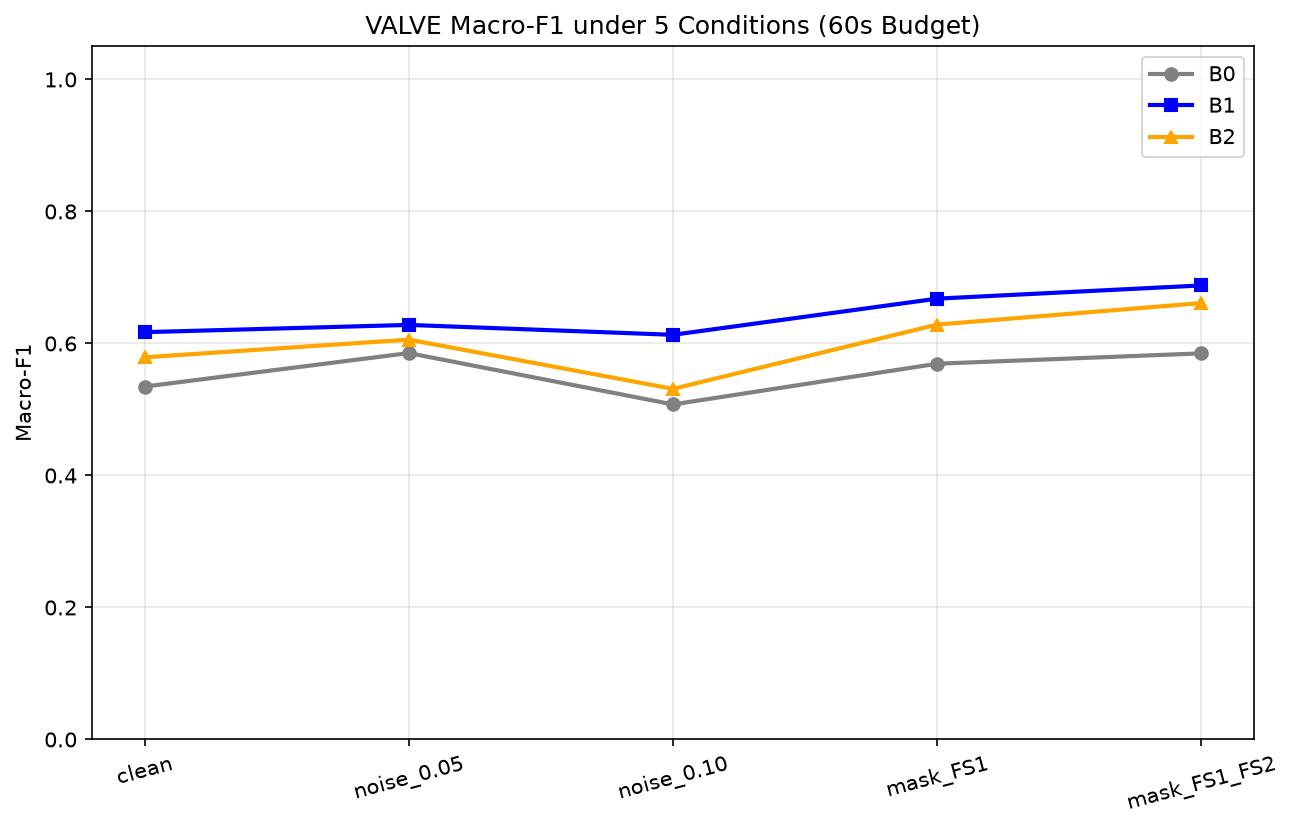
\includegraphics[width=\textwidth]{figures/robustness_valve_60s.png}
        \caption{阀门部件鲁棒性比较}
        \label{fig:robustness_valve}
    \end{subfigure}
    
    % 第二行两张子图
    \vspace{0.5cm}
    \begin{subfigure}[b]{0.45\textwidth}
        \centering
        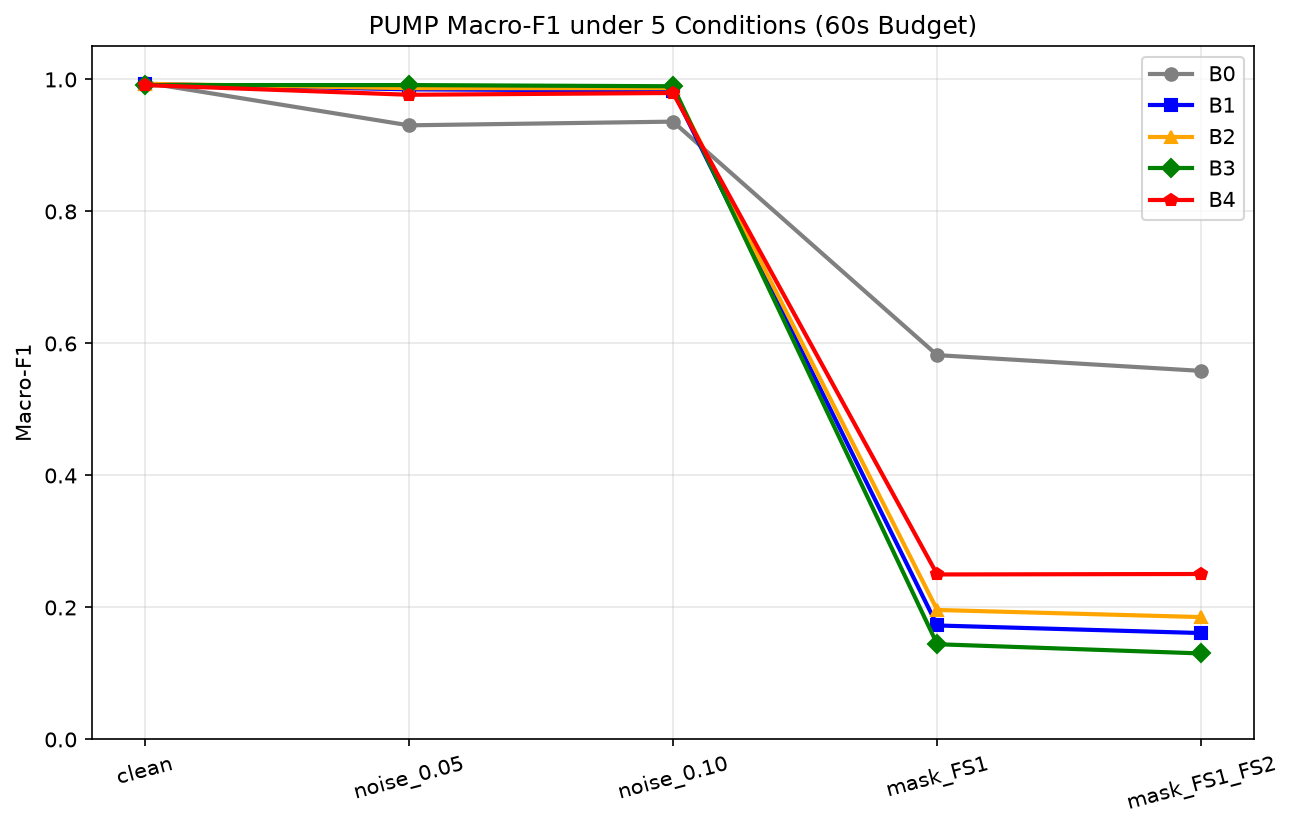
\includegraphics[width=\textwidth]{figures/robustness_pump_60s.png}
        \caption{泵部件鲁棒性比较}
        \label{fig:robustness_pump}
    \end{subfigure}
    \hfill
    \begin{subfigure}[b]{0.45\textwidth}
        \centering
        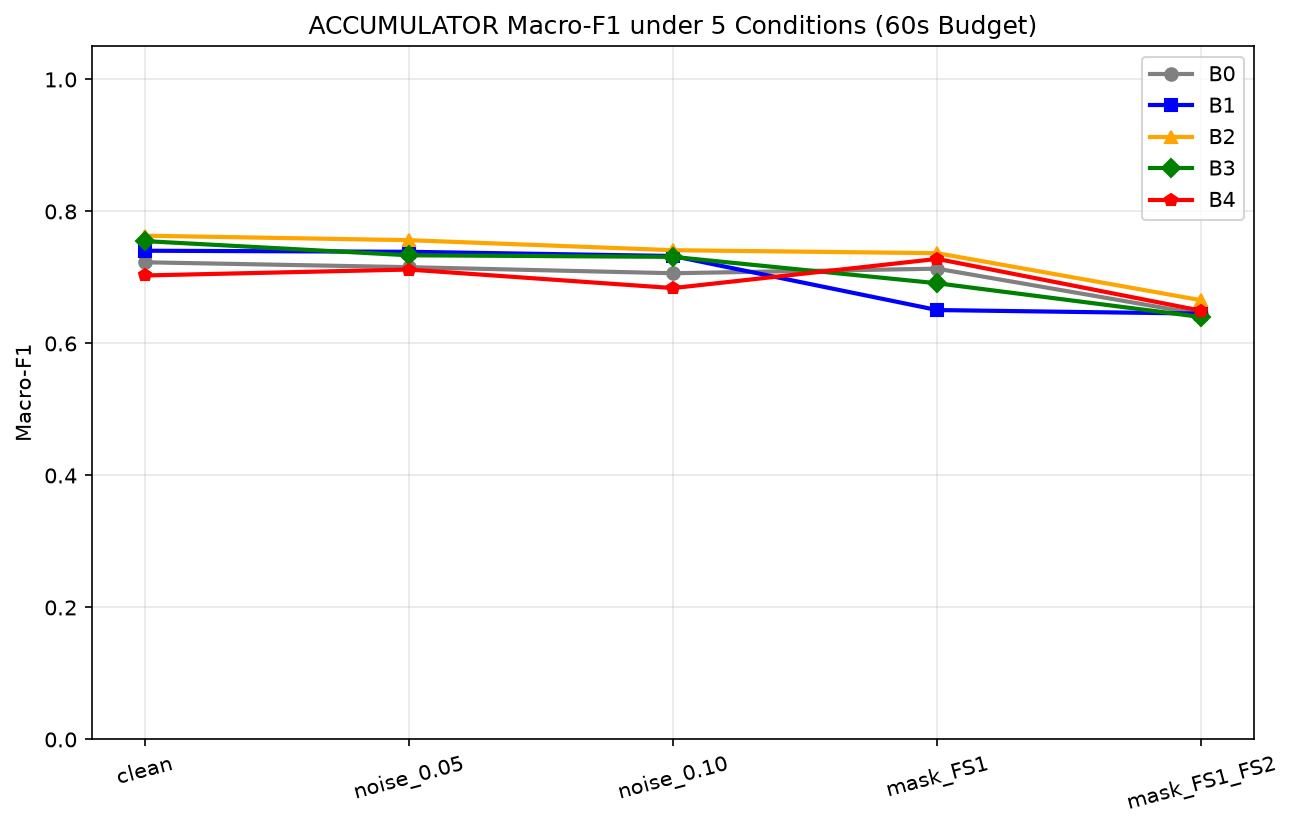
\includegraphics[width=\textwidth]{figures/robustness_accumulator_60s.png}
        \caption{蓄能器部件鲁棒性比较}
        \label{fig:robustness_accumulator}
    \end{subfigure}
    
    % 总标题与总标签
    \caption{四部件不同工况下鲁棒性折线图}
    \label{fig:robustness_all}
\end{figure}
\begin{table}[H]
    \centering
    \caption{10秒观测预算下五种测试条件的四部件平均Macro-F1}
    \label{tab:robust_10s}
    \small
    \begin{tabular}{lccccc}
        \toprule
        \textbf{模型} & \textbf{无扰动} & \textbf{噪声0.05} & \textbf{噪声0.10} & \textbf{屏蔽FS1} & \textbf{屏蔽FS1+FS2} \\
        \midrule
        B0 & 0.8738 & 0.8353 & 0.8160 & 0.8750 & 0.8540 \\
        B1 & 0.9063 & 0.8776 & 0.8723 & 0.9123 & 0.9008 \\
        B2 & 0.9010 & 0.8896 & 0.8768 & 0.9081 & 0.8909 \\
        B3 & 0.9061 & 0.8911 & 0.8618 & 0.9070 & 0.9016 \\
        B4 & 0.8700 & 0.7944 & 0.7891 & 0.8807 & 0.8624 \\
        \bottomrule
    \end{tabular}
\end{table}
\begin{table}[H]
    \centering
    \caption{30秒观测预算下五种测试条件的四部件平均Macro-F1}
    \label{tab:robust_30s}
    \small
    \begin{tabular}{lccccc}
        \toprule
        \textbf{模型} & \textbf{无扰动} & \textbf{噪声0.05} & \textbf{噪声0.10} & \textbf{屏蔽FS1} & \textbf{屏蔽FS1+FS2} \\
        \midrule
        B0 & 0.8020 & 0.8000 & 0.7885 & 0.6367 & 0.6249 \\
        B1 & 0.9010 & 0.8909 & 0.8732 & 0.7129 & 0.6964 \\
        B2 & 0.8806 & 0.8734 & 0.8603 & 0.6653 & 0.6662 \\
        B3 & 0.8939 & 0.8851 & 0.8702 & 0.6956 & 0.6788 \\
        B4 & 0.8162 & 0.8241 & 0.7961 & 0.6208 & 0.6032 \\
        \bottomrule
    \end{tabular}
\end{table}
\begin{table}[H]
    \centering
    \caption{60秒观测预算下五种测试条件的四部件平均Macro-F1}
    \label{tab:robust_60s}
    \small
    \begin{tabular}{lccccc}
        \toprule
        \textbf{模型} & \textbf{无扰动} & \textbf{噪声0.05} & \textbf{噪声0.10} & \textbf{屏蔽FS1} & \textbf{屏蔽FS1+FS2} \\
        \midrule
        B0 & 0.8104 & 0.8051 & 0.7825 & 0.7134 & 0.6941 \\
        B1 & 0.8355 & 0.8358 & 0.8299 & 0.6205 & 0.6213 \\
        B2 & 0.8311 & 0.8350 & 0.8120 & 0.6376 & 0.6252 \\
        B3 & 0.8344 & 0.8363 & 0.8293 & 0.6143 & 0.6017 \\
        B4 & 0.8113 & 0.8112 & 0.7885 & 0.6412 & 0.6264 \\
        \bottomrule
    \end{tabular}
\end{table}
为完整对齐任务书对鲁棒性实验的要求，除四部件平均Macro-F1外，下表进一步给出五种测试条件下的逐部件结果、异常定位F1与告警F1。五种条件均以固定随机种子、按训练集标准差生成同一扰动序列，10/30/60秒共用该序列进行一致回放，保证扰动实现与结果完全可复现。

从逐部件结果看，加噪场景下各部件性能衰减温和且改进方案始终优于基线：0.10倍强噪声下阀门 Macro-F1为 B0 0.5076、B1 0.6131，冷却器在所有场景下稳定在0.98以上，印证了温度类故障的稳态特性。真正的性能悬崖出现在传感器屏蔽场景：FS1被屏蔽后泵的Macro-F1由接近1.0骤降至 0.13--0.58，且B0（0.5823）反而略优于引入流量类特征的改进方案，与前述"物理依赖软肋"的结论一致。

异常定位F1与告警F1呈现出与Macro-F1不同的敏感性。在加噪场景下二者几乎不衰减，B1/B3的告警 F1仍保持在0.94以上、异常定位F1保持在0.87以上，说明均值型统计量与防抖状态机对高频噪声有天然的平滑作用。而在屏蔽FS1时，各方案异常定位F1由约0.87降至0.75--0.82、告警F1由约0.86--0.96降至0.75--0.82，健康部件误报率同步升高（如B1由3.9\% 升至30.6\%）：泵的流量特征失效后，模型在正常周期上也会输出异常等级，经连续双时点确认后仍形成正式告警，从而抬高误报。需要指出的是，在FS1屏蔽场景下B1/B3的告警F1（约0.82）仍略高于基线B0（0.8118），但B2因缺少差分特征而略低于B0（0.7882与0.8118）；在同时屏蔽FS1+FS2时B1/B2/B3均高于B0。可见分段时序特征带来的告警收益在多数扰动下稳健，但并非在所有场景都绝对占优，该负结果与泵对流量通道的强物理依赖相互印证。
\begin{table}[H]
    \centering
    \caption{60秒观测预算下五种测试条件的逐部件 Macro-F1}
    \label{tab:robust_percomp}
    \small
    \begin{tabular}{llcccc}
        \toprule
        \textbf{测试条件} & \textbf{模型} & \textbf{冷却器} & \textbf{阀门} & \textbf{泵} & \textbf{蓄能器} \\
        \midrule
        \multirow{5}{*}{无扰动}
            & B0 & 0.9888 & 0.5347 & 0.9953 & 0.7230 \\
            & B1 & 0.9910 & 0.6171 & 0.9934 & 0.7405 \\
            & B2 & 0.9888 & 0.5790 & 0.9934 & 0.7633 \\
            & B3 & 0.9910 & 0.6001 & 0.9915 & 0.7551 \\
            & B4 & 0.9910 & 0.5595 & 0.9915 & 0.7030 \\
        \midrule
        \multirow{5}{*}{噪声0.05}
            & B0 & 0.9888 & 0.5854 & 0.9305 & 0.7156 \\
            & B1 & 0.9910 & 0.6281 & 0.9850 & 0.7389 \\
            & B2 & 0.9910 & 0.6058 & 0.9868 & 0.7565 \\
            & B3 & 0.9910 & 0.6290 & 0.9915 & 0.7336 \\
            & B4 & 0.9910 & 0.5651 & 0.9768 & 0.7120 \\
        \midrule
        \multirow{5}{*}{噪声0.10}
            & B0 & 0.9799 & 0.5076 & 0.9361 & 0.7064 \\
            & B1 & 0.9910 & 0.6131 & 0.9831 & 0.7325 \\
            & B2 & 0.9888 & 0.5312 & 0.9868 & 0.7413 \\
            & B3 & 0.9910 & 0.6053 & 0.9897 & 0.7312 \\
            & B4 & 0.9880 & 0.5026 & 0.9795 & 0.6839 \\
        \midrule
        \multirow{5}{*}{屏蔽FS1}
            & B0 & 0.9888 & 0.5693 & 0.5823 & 0.7133 \\
            & B1 & 0.9910 & 0.6679 & 0.1727 & 0.6506 \\
            & B2 & 0.9888 & 0.6286 & 0.1962 & 0.7368 \\
            & B3 & 0.9910 & 0.6307 & 0.1443 & 0.6912 \\
            & B4 & 0.9910 & 0.5955 & 0.2500 & 0.7281 \\
        \midrule
        \multirow{5}{*}{屏蔽FS1+FS2}
            & B0 & 0.9888 & 0.5850 & 0.5584 & 0.6441 \\
            & B1 & 0.9910 & 0.6879 & 0.1612 & 0.6452 \\
            & B2 & 0.9888 & 0.6612 & 0.1854 & 0.6654 \\
            & B3 & 0.9910 & 0.6453 & 0.1303 & 0.6400 \\
            & B4 & 0.9910 & 0.6145 & 0.2507 & 0.6495 \\
        \bottomrule
    \end{tabular}
\end{table}
\begin{table}[H]
    \centering
    \caption{五种测试条件下各方案的异常定位 F1（60秒，异常/正常二值口径，池化四部件）}
    \label{tab:robust_loc_f1}
    \small
    \begin{tabular}{lccccc}
        \toprule
        \textbf{模型} & \textbf{无扰动} & \textbf{噪声0.05} & \textbf{噪声0.10} & \textbf{屏蔽FS1} & \textbf{屏蔽FS1+FS2} \\
        \midrule
        B0 & 0.8626 & 0.8626 & 0.8563 & 0.8215 & 0.8132 \\
        B1 & 0.8790 & 0.8853 & 0.8827 & 0.7496 & 0.7786 \\
        B2 & 0.8776 & 0.8841 & 0.8700 & 0.7737 & 0.7865 \\
        B3 & 0.8730 & 0.8778 & 0.8758 & 0.7442 & 0.7513 \\
        B4 & 0.8621 & 0.8644 & 0.8481 & 0.7726 & 0.7786 \\
        \bottomrule
    \end{tabular}
\end{table}
\begin{table}[H]
    \centering
    \caption{五种测试条件下各方案的告警 F1（跨10/30/60秒同一扰动一致回放，"周期--部件"对口径）}
    \label{tab:robust_alarm_f1}
    \small
    \begin{tabular}{lccccc}
        \toprule
        \textbf{模型} & \textbf{无扰动} & \textbf{噪声0.05} & \textbf{噪声0.10} & \textbf{屏蔽FS1} & \textbf{屏蔽FS1+FS2} \\
        \midrule
        B0 & 0.8616 & 0.8634 & 0.8589 & 0.8118 & 0.8046 \\
        B1 & 0.9606 & 0.9498 & 0.9400 & 0.8192 & 0.8121 \\
        B2 & 0.9405 & 0.9395 & 0.9240 & 0.7882 & 0.8139 \\
        B3 & 0.9597 & 0.9499 & 0.9394 & 0.8183 & 0.8097 \\
        B4 & 0.8681 & 0.8751 & 0.8404 & 0.7544 & 0.7649 \\
        \bottomrule
    \end{tabular}
\end{table}
\section{系统评测结果}
\subsection{主结果与稳定性分层}
为了更细致地评估模型在各个具体健康等级上的表现，下表汇总了五种方案在60秒完整周期下、测试集中各部件状态的样本数与逐类召回率（Recall）。
从数据中可以观察到几个显著现象：泵的识别率极高，所有方案在泵的三个状态上均保持在98\%以上的极高召回率，这说明泵的内泄漏特征在压力与功率信号中体现得非常明显，极易被模型捕捉。阀门具有长窗口困境，所有模型对阀门状态90的召回率均停留在0.400，且状态100的召回率较低。这印证了前文的失败分析：60秒长窗口使得阀门的早期瞬态特征被稳态信号稀释，导致正常（100）与轻微滞后（90）极易互相混淆。对比B0，引入时序分段特征的B1和B3在阀门状态80和100上的召回率有显著提升；同时，B2在蓄能器状态130的召回率（0.804）显著优于B0（0.707），证明分段均值有效保留了长效状态的趋势特征。
\begin{table}[H]
    \centering
    \caption{各模型在 60 秒无扰动条件下的逐等级 Recall 与样本数}
    \label{tab:recall_per_class}
    \small
    \setlength{\tabcolsep}{6pt}
    \begin{tabular}{llcccccc}
        \toprule
        \multirow{2}{*}{\textbf{部件}} & \multirow{2}{*}{\textbf{等级}} & \multirow{2}{*}{\textbf{样本数}} & \multicolumn{5}{c}{\textbf{各模型 Recall}} \\
        \cmidrule(lr){4-8}
        & & & \textbf{B0} & \textbf{B1} & \textbf{B2} & \textbf{B3} & \textbf{B4} \\
        \midrule
        \multirow{3}{*}{冷却器} & 3   & 133 & 1.000 & 1.000 & 1.000 & 1.000 & 1.000 \\
                                & 20  &  93 & 1.000 & 1.000 & 1.000 & 1.000 & 1.000 \\
                                & 100 & 333 & 0.985 & 0.988 & 0.985 & 0.988 & 0.988 \\
        \midrule
        \multirow{4}{*}{阀门} & 73  &  70 & 0.957 & 0.971 & 0.957 & 0.957 & 0.957 \\
                              & 80  &  70 & 0.571 & 0.800 & 0.643 & 0.814 & 0.686 \\
                              & 90  &  50 & 0.400 & 0.400 & 0.400 & 0.400 & 0.400 \\
                              & 100 & 369 & 0.293 & 0.407 & 0.388 & 0.360 & 0.309 \\
        \midrule
        \multirow{3}{*}{泵} & 0   & 394 & 1.000 & 0.998 & 0.998 & 0.995 & 0.995 \\
                            & 1   & 113 & 1.000 & 1.000 & 1.000 & 1.000 & 1.000 \\
                            & 2   &  52 & 0.981 & 0.981 & 0.981 & 0.981 & 0.981 \\
        \midrule
        \multirow{4}{*}{蓄能器} & 90  & 313 & 0.796 & 0.824 & 0.818 & 0.824 & 0.799 \\
                                & 100 &  71 & 0.747 & 0.732 & 0.761 & 0.761 & 0.704 \\
                                & 115 &  83 & 0.735 & 0.735 & 0.747 & 0.759 & 0.735 \\
                                & 130 &  92 & 0.707 & 0.728 & 0.804 & 0.750 & 0.652 \\
        \bottomrule
    \end{tabular}
\end{table}
下表展示B0至B4五个不同测试对象在完整周期60秒时间预算下的主结果，包含逐部件Macro-F1，四部件均值，异常定位F1和告警F1。
\begin{table}[H]
    \centering
    \caption{各模型在60秒观测预算下的主结果}
    \label{tab:main_results_60s}
    \begin{tabular}{lccccccc}
        \toprule
        \multirow{2}{*}{\textbf{模型}} & \multicolumn{4}{c}{\textbf{逐部件 Macro-F1}} & \multirow{2}{*}{\textbf{四部件均值}} & \multirow{2}{*}{\textbf{异常定位 F1}} & \multirow{2}{*}{\textbf{告警 F1}} \\
        \cmidrule(lr){2-5}
                       & \textbf{冷却器} & \textbf{阀门} & \textbf{泵} & \textbf{蓄能器} &         &         &         \\
        \midrule
        B0             & 0.9888 & 0.5347 & 0.9953 & 0.7230 & 0.8104 & 0.8626 & 0.8616 \\
        B1             & 0.9910 & 0.6171 & 0.9934 & 0.7405 & 0.8355 & 0.8790 & 0.9606 \\
        B2             & 0.9888 & 0.5790 & 0.9934 & 0.7633 & 0.8311 & 0.8776 & 0.9405 \\
        B3             & 0.9910 & 0.6001 & 0.9915 & 0.7551 & 0.8344 & 0.8730 & 0.9597 \\
        B4             & 0.9910 & 0.5595 & 0.9915 & 0.7030 & 0.8113 & 0.8621 & 0.8681 \\
        \bottomrule
    \end{tabular}
\end{table}
针对不同时间预算下的指标汇总如下表所示，总结得出短时间预算10秒时所有方案的严格联合准确率都达到0.68以上，B1、B2、B3突破0.75。短窗口下信号的瞬态故障特征能量集中，没有长窗口的平均化稀释效应，所有模型都能快速做出准确判断。中时间预算30秒时性能出现明显分化。B1、B2、B3的平均Macro-F1依然维持在0.88以上，而B0与B4直接暴跌到0.80左右，严格联合准确率更是从0.69跌到0.26。这直接证明：‌纯全局统计特征完全无法应对30秒以上的长窗口，时序分段特征是长窗口下维持性能的必要条件‌。长时间预算60秒下所有方案的严格联合准确率都出现断崖式下跌，B1也仅为0.3596。这是因为60秒长窗口下，系统状态多次切换，同时出现多个部件的复合故障概率大幅提升，要求模型同时对4个部件的状态全部预测正确，难度呈指数级上升。
\begin{table}[H]
    \centering
    \caption{无扰动条件下各模型在10/30/60秒观测预算的诊断性能对照}
    \label{tab:clean_budget_compare}
    \small
    \begin{tabular}{lcccccc}
        \toprule
        \multirow{2}{*}{\textbf{模型}} & \multicolumn{2}{c}{\textbf{10 秒}} & \multicolumn{2}{c}{\textbf{30 秒}} & \multicolumn{2}{c}{\textbf{60 秒}} \\
        \cmidrule(lr){2-3} \cmidrule(lr){4-5} \cmidrule(lr){6-7}
                       & \textbf{平均F1} & \textbf{联合准确率} & \textbf{平均 F1} & \textbf{联合准确率} & \textbf{平均F1} & \textbf{联合准确率} \\
        \midrule
        B0             & 0.8738 & 0.6941 & 0.8020 & 0.2630 & 0.8104 & 0.2665 \\
        B1             & 0.9063 & 0.7674 & 0.9010 & 0.7048 & 0.8355 & 0.3596 \\
        B2             & 0.9010 & 0.7531 & 0.8806 & 0.6100 & 0.8311 & 0.3363 \\
        B3             & 0.9061 & 0.7692 & 0.8939 & 0.6995 & 0.8344 & 0.3256 \\
        B4             & 0.8700 & 0.6852 & 0.8162 & 0.2898 & 0.8113 & 0.2719 \\
        \bottomrule
    \end{tabular}
\end{table}
稳定性分层结果如下表所示。稳定周期（flag=0）中所有方案的联合准确率都远高于未稳定周期（flag=1），B3在稳定周期下甚至达到0.5485。这一现象与直觉相符：当系统处于过渡态、扰动态时，各传感器的信号本身在剧烈变化，这种物理上的非平稳性导致各种故障特征完全被淹没在动态噪声中，模型极难区分系统正常的过渡波动与真实的早期故障，导致所有方案的性能都出现大幅下降，B1最高也仅为0.1538。相反，在稳定周期中，虽然故障特征较为微弱，但系统工况相对平稳，模型的决策边界更加清晰。B3和B1在稳定周期下的性能是所有方案中最高的（均超过0.53），说明它们的差分特征能捕捉到稳态下极其细微的信号变化，对平稳期早期故障的识别能力最强。
\begin{table}[H]
    \centering
    \caption{各模型在60秒预算下的联合准确率与稳定性分层}
    \label{tab:joint_acc_60s}
    \begin{tabular}{lcccc}
        \toprule
        \textbf{模型} & \textbf{严格联合准确率} & \textbf{稳定周期 (flag=0)} & \textbf{未稳定周期 (flag=1)} & \textbf{漏报数} \\
        \midrule
        B0           & 0.2665        & 0.4482            & 0.0577           & 46    \\
        B1           & 0.3596        & 0.5385            & 0.1538           & 37    \\
        B2           & 0.3363        & 0.5184            & 0.1269           & 29    \\
        B3           & 0.3256        & 0.5485            & 0.0692           & 37    \\
        B4           & 0.2719        & 0.4548            & 0.0615           & 44    \\
        \bottomrule
    \end{tabular}
\end{table}
针对全正常组合的误报测试，原始数据中该组合仅有21个周期，同时报告了周期粒度和部件粒度的误报个数与分母。具体结果如下表所示。由于全正常组合完全未参与训练，所有模型均出现了不同程度的误报。其中B2的周期粒度误报率最低（66.7\%），而B0和B4在21个正常周期中全部发生了误报。这表明缺乏时序分段特征的模型（B0/B4）在面对未见过的全正常复合工况时，极易将正常的系统扰动误判为异常。
\begin{table}[H]
    \centering
    \caption{全正常组合（21个周期）误报数统计与分母}
    \label{tab:false_alarm}
    \small
    \setlength{\tabcolsep}{3pt}
    \begin{tabular}{lcccccc}
        \toprule
        \multirow{2}{*}{\textbf{模型}} & \multirow{2}{*}{\textbf{全正常周期数}} & \multicolumn{2}{c}{\textbf{周期粒度}} & \multicolumn{2}{c}{\textbf{部件粒度}} & \multirow{2}{*}{\textbf{正式误报告警周期数}} \\
        \cmidrule(lr){3-4} \cmidrule(lr){5-6}
        & & \textbf{误报数} & \textbf{误报率} & \textbf{误报数} & \textbf{误报率} & \\
        \midrule
        B0 & 21 & 21 & 100.0\% & 39 & 46.4\% (39/84) & 19 \\
        B1 & 21 & 16 & 76.2\%  & 26 & 31.0\% (26/84) & 19 \\
        B2 & 21 & 14 & 66.7\%  & 24 & 28.6\% (24/84) & 15 \\
        B3 & 21 & 16 & 76.2\%  & 26 & 31.0\% (26/84) & 18 \\
        B4 & 21 & 21 & 100.0\% & 33 & 39.3\% (33/84) & 19 \\
        \bottomrule
    \end{tabular}
\end{table}
为了进一步分析系统的告警响应能力，下表统计了各模型在正确触发告警时的观测时长分布与漏报情况。数据表明，引入分段时序特征的改进方案（B1、B2、B3）在告警性能上取得了显著突破，其Alarm-F1 均跃升至0.94以上，而基线模型（B0、B4）仅为0.86左右。在响应速度方面，B3模型表现出极快的异常捕获能力，有95.1\%的正确告警在观测的第30秒内即已完成输出，而B0仅有89.8\%同时，漏报数从基线的46次大幅降低至B1/B3的37次，B2降至29次。这证明分段统计与差分特征有效放大了早期微弱故障信号，使得防抖状态机能够更早、更准确地确认异常，极大降低了工业场景下的安全风险。
\begin{table}[H]
    \centering
    \caption{各模型告警时长分布与漏报统计（60秒预算）}
    \label{tab:alarm_time_dist}
    \small
    \setlength{\tabcolsep}{4pt}
    \begin{tabular}{lcccccc}
        \toprule
        \textbf{模型} & \textbf{Alarm\_F1} & \textbf{30秒内告警数} & \textbf{60秒告警数} & \textbf{正确告警总数} & \textbf{30秒内占比} & \textbf{漏报数} \\
        \midrule
        B0 & 0.8616 & 900 & 102 & 1002 & 89.8\% & 46 \\
        B1 & 0.9606 & 947 &  64 & 1011 & 93.7\% & 37 \\
        B2 & 0.9405 & 955 &  64 & 1019 & 93.7\% & 29 \\
        B3 & 0.9597 & 961 &  50 & 1011 & 95.1\% & 37 \\
        B4 & 0.8681 & 898 & 106 & 1004 & 89.4\% & 44 \\
        \bottomrule
    \end{tabular}
\end{table}
为了完整刻画告警质量，下表在"周期--部件"对口径上给出各模型的告警 Precision、Recall、F1、健康部件误报率与告警等级准确率。可见改进方案在保持高召回的同时大幅压低了误报：B1 将健康部件误报率从基线 B0 的 23.2\% 降至 3.9\%，告警 Precision 从 0.7840 提升至 0.9565，且告警等级的判定准确率由 0.6878 提升至 0.8761，说明分段时序特征不仅让告警更早触发，也让告警所报等级更可靠。
需要特别说明的是，下表中的"首次告警时间"表示从周期开始到形成正式告警所使用的观测时长，刻画的是达到可靠诊断所需的观测窗口长度，并非真实故障发生到告警的延迟；本任务不评价该延迟，亦不据此声称系统能够提前发现真实故障。
\begin{table}[H]
    \centering
    \caption{各模型告警完整指标（60秒预算，"周期--部件"对口径）}
    \label{tab:alarm_full}
    \small
    \setlength{\tabcolsep}{4pt}
    \begin{tabular}{lccccc}
        \toprule
        \textbf{模型} & \textbf{告警Precision} & \textbf{告警Recall} & \textbf{告警F1} & \textbf{健康部件误报率} & \textbf{告警等级准确率} \\
        \midrule
        B0 & 0.7840 & 0.9561 & 0.8616 & 276/1188 = 23.2\% & 0.6878 \\
        B1 & 0.9565 & 0.9647 & 0.9606 & 46/1188 = 3.9\%   & 0.8761 \\
        B2 & 0.9106 & 0.9723 & 0.9405 & 100/1188 = 8.4\%  & 0.8293 \\
        B3 & 0.9547 & 0.9647 & 0.9597 & 48/1188 = 4.0\%   & 0.8744 \\
        B4 & 0.7937 & 0.9580 & 0.8681 & 261/1188 = 22.0\% & 0.6988 \\
        \bottomrule
    \end{tabular}
\end{table}
从下表可以看出三个核心结论：冷却器、泵、蓄能器三个部件的分类性能接近完美：所有方案F1值均在0.95以上，泵的Recall达到1.0，不存在漏判；阀门是所有方案共同的性能瓶颈，F1值仅在0.55到0.59之间，核心原因是阀门相邻滞后等级（80/90/100）的波形差异仅为亚秒级切换沿陡度，当前统计特征难以捕捉；B1方案综合性能最优：阀门F1比基线B0提升4个百分点，同时保持泵和蓄能器的高精度，验证了分段差分特征的有效性。测试集共包含559个完整周期，四个部件标签样本数均为559，各故障等级的逐类Recall已标注于各个模型汇总的归一化混淆矩阵对角线中，括号内为该等级实际样本数。
\begin{table}[H]
  \centering
  \caption{60秒观测预算下五种方案的逐部件异常定位性能对比（正常/异常二分类，"周期--部件"对口径）}
  \label{tab:part_prf}
  \small
  \setlength{\tabcolsep}{6pt}
  \begin{tabular}{llccc}
    \toprule
    特征方案 & 部件 & Precision & Recall & F1-score \\
    \midrule
    \multirow{4}{*}{B0} & 冷却器 & 0.9784 & 1.0000 & 0.9891 \\
                        & 阀门   & 0.3944 & 0.8947 & 0.5475 \\
                        & 泵     & 1.0000 & 1.0000 & 1.0000 \\
                        & 蓄能器 & 0.9441 & 0.9764 & 0.9600 \\
    \midrule
    \multirow{4}{*}{B1} & 冷却器 & 0.9826 & 1.0000 & 0.9912 \\
                        & 阀门   & 0.4370 & 0.8947 & 0.5872 \\
                        & 泵     & 0.9940 & 1.0000 & 0.9970 \\
                        & 蓄能器 & 0.9480 & 0.9764 & 0.9620 \\
    \midrule
    \multirow{4}{*}{B2} & 冷却器 & 0.9784 & 1.0000 & 0.9891 \\
                        & 阀门   & 0.4307 & 0.9000 & 0.5826 \\
                        & 泵     & 0.9940 & 1.0000 & 0.9970 \\
                        & 蓄能器 & 0.9618 & 0.9700 & 0.9659 \\
    \midrule
    \multirow{4}{*}{B3} & 冷却器 & 0.9826 & 1.0000 & 0.9912 \\
                        & 阀门   & 0.4201 & 0.9000 & 0.5729 \\
                        & 泵     & 0.9880 & 1.0000 & 0.9940 \\
                        & 蓄能器 & 0.9519 & 0.9743 & 0.9630 \\
    \midrule
    \multirow{4}{*}{B4} & 冷却器 & 0.9826 & 1.0000 & 0.9912 \\
                        & 阀门   & 0.4000 & 0.8947 & 0.5528 \\
                        & 泵     & 0.9880 & 1.0000 & 0.9940 \\
                        & 蓄能器 & 0.9343 & 0.9743 & 0.9539 \\
    \bottomrule
  \end{tabular}
\end{table}

\subsection{工程性能与因果检查}
\subsubsection{工程性能测试结果}
下表展示工程性能基准测试主结果，使用完整周期时间预算。耗时构成中端到端P50为48.2到50.9ms‌，其中特征提取仅1.0到1.6ms‌。特征提取占比 ‌2.1\%到3.2\%，随机森林推断占96.8\%到97.9\%，瓶颈在于模型端。五种不同模型方案中，特征提取耗时随特征维度单调上升。B0/B4（低维）‌0.8-1.2ms‌到B1/B2（中维）‌1.1-1.4ms‌到B3（最高维）‌1.6-3.2ms‌。推断耗时在五方案间差异不足 6\%（46.8到49.7ms），说明推断成本由4个部件与200棵树的固定遍历次数决定，与特征维度基本无关。增加特征的代价只体现在特征提取上，而这一项本身占端到端不到3\%，因此‌特征方案应完全按精度选型，不必做速度取舍‌。模型体积和训练成本而言体积与特征维度‌负相关‌：B3（最高维）‌5.24MB‌最小，B0（最低维）‌6.35 MB‌最大。原因是特征维度高时单次分裂信息量更足，树可以更浅、节点更少，因此参数矩阵反而更小。体积与训练时间都在 MB 级与秒级，属一次性离线成本，不构成部署约束。
\begin{table}[H]
  \centering
  \caption{工程性能基准测试主结果（观测窗口 60\,s，测试集20个周期重复测量）}
  \label{tab:bench_60s}
  \small
  \setlength{\tabcolsep}{5pt}
  \begin{tabular}{lccccccc}
    \toprule
    \multirow{2}{*}{特征方案} & 训练耗时 & 特征提取 & 特征提取 & 模型推断 & 端到端 & 端到端 & 模型体积 \\
                              & (s)      & P50 (ms) & P95 (ms) & P50 (ms) & P50 (ms) & P95 (ms) & (MB) \\
    \midrule
    B0 & 3.63 & 1.04 & 1.33 & 47.35 & 48.40 & 59.94 & 6.35 \\
    B1 & 4.11 & 1.36 & 1.50 & 46.84 & 48.20 & 61.27 & 5.42 \\
    B2 & 4.03 & 1.39 & 1.57 & 48.99 & 50.38 & 67.82 & 5.54 \\
    B3 & 4.04 & 1.63 & 3.22 & 48.70 & 50.33 & 62.62 & 5.24 \\
    B4 & 3.99 & 1.15 & 1.36 & 49.70 & 50.86 & 65.65 & 6.01 \\
    \bottomrule
  \end{tabular}
\end{table}
此外评估系统在边缘计算节点上的部署可行性使用Python的tracemalloc模块对单周期推理的内存峰值进行了测量。如下表所示，所有方案在所有观测预算下的总内存峰值均极低，稳定在0.31MB到0.49MB 之间。随着观测预算从10秒增加到60秒，特征提取阶段的内存峰值从0.02MB 微增至0.1MB，模型推断阶段的内存峰值从约0.29MB增至约0.39MB，总体增幅不到0.2MB。这主要是因为窗口越长，参与计算的原始数据矩阵越大，相对于现代工控机或边缘设备其内存开销完全可以忽略不计。这种极低的内存占用得益于随机森林算法高效的树结构遍历机制，也证明了本系统在实际工业现场进行实时、连续状态监测方面具备极高的工程部署价值。
\begin{table}[H]
    \centering
    \caption{各方案在不同观测预算下的单周期内存峰值统计}
    \label{tab:memory_peak}
    \small
    \setlength{\tabcolsep}{4pt}
    \begin{tabular}{lcccc}
        \toprule
        \textbf{模型} & \textbf{秒预算} & \textbf{特征提取内存峰值(MB)} & \textbf{模型推断内存峰值(MB)} & \textbf{合计内存峰值(MB)} \\
        \midrule
        \multirow{3}{*}{B0} & 10 & 0.02 & 0.29 & 0.31 \\
                            & 30 & 0.05 & 0.31 & 0.36 \\
                            & 60 & 0.10 & 0.36 & 0.46 \\
        \midrule
        \multirow{3}{*}{B1} & 10 & 0.02 & 0.30 & 0.32 \\
                            & 30 & 0.05 & 0.33 & 0.38 \\
                            & 60 & 0.10 & 0.38 & 0.48 \\
        \midrule
        \multirow{3}{*}{B2} & 10 & 0.02 & 0.31 & 0.33 \\
                            & 30 & 0.05 & 0.36 & 0.41 \\
                            & 60 & 0.10 & 0.39 & 0.49 \\
        \midrule
        \multirow{3}{*}{B3} & 10 & 0.02 & 0.31 & 0.33 \\
                            & 30 & 0.05 & 0.33 & 0.38 \\
                            & 60 & 0.10 & 0.37 & 0.47 \\
        \midrule
        \multirow{3}{*}{B4} & 10 & 0.02 & 0.29 & 0.31 \\
                            & 30 & 0.05 & 0.31 & 0.36 \\
                            & 60 & 0.10 & 0.35 & 0.45 \\
        \bottomrule
    \end{tabular}
\end{table}
\subsubsection{因果校验验证结果}
对于因果性校验，本系统的诊断严格遵循预测时刻能够看到的数据只有观测窗口内的前缀，训练时使用的统计量仅来自于训练集。对于时间前缀泄露的问题本系统构造时使用严格切片:fs*seconds实现，对于未来信息意外读入使用扰动窗口外数据验证输出不变进行验证。对于填充统计量泄露问题中位数仅由训练集计算并写入元数据，对于训练集测试集周期泄露问题严格使用周期划分的manifest.csv防止同一周期出现在训练和测试。

对于扰动验证伪代码如下所示，在10秒与30秒两种预算、五种特征方案共10组配置上执行校验，全部10组均满足窗口外数据被替换为随机扰动后，特征矩阵逐元素相等、四个部件的预测标签全部不变。由此确认前缀截断实现的正确性，以及回放倍率切换不会改变单周期诊断结论。

此外，缺失值补偿所用的中位数完全由训练集计算并固化于模型元数据，回放与评测阶段直接复用、绝不依据测试数据重算；告警状态机在每个周期开始时重置候选池与告警计数，仅使用当前及更早观测时点的预测，不使用任何未来时点信息或前一周期状态。由此，特征计算、缺失补偿、模型推理与告警状态四个环节均通过了前缀因果性校验。
\begin{lstlisting}[language=Python, caption=基于窗口外扰动的因果性校验核心逻辑]
def causality_check(raw_data, budget_T, cycle_id, extract_fn, model):
    # 基线特征：仅使用窗口内的前缀数据
    x_prefix = raw_data[cycle_id, :budget_T]
    feat_base = extract_fn(x_prefix)
    pred_base = model.predict(feat_base)
    
    # 扰动数据：将窗口外 (T时刻之后) 的数据替换为随机噪声
    perturbed_data = raw_data[cycle_id].copy()
    perturbed_data[budget_T:] = np.random.normal(0, 10, len(perturbed_data[budget_T:]))
    
    # 扰动特征：再次提取窗口内特征并预测
    x_prefix_perturbed = perturbed_data[:budget_T]
    feat_perturbed = extract_fn(x_prefix_perturbed)
    pred_perturbed = model.predict(feat_perturbed)
    
    # 校验断言：前缀特征应保持不变，且预测标签一致
    assert np.allclose(feat_base, feat_perturbed), "特征发生泄漏"
    assert pred_base == pred_perturbed, "预测结果发生漂移"
    return True
\end{lstlisting}
\section{错误案例分析}
以下展示通过代码寻找的告警与真实标签不一致部分典型错误案例进行分析。5个误判周期均取自B1方案在60秒窗口下的测试集预测结果，每图给出该周期参与决策的关键传感器原始波形，观测时长60秒，横轴为观测时间。总体而言，边界错误占比最高，无跨等级的严重错误，说明模型整体故障方向判断正确，仅在等级细分上存在误差。瞬态与非稳态是主要误差来源‌：未热平衡周期、阀切换瞬态尖峰、传感器噪声等非稳态因素，是导致特征混淆的核心原因。所有误判案例中，防抖告警逻辑均未触发严重误报：相邻等级错误不会触发告警或仅触发低等级告警，满足工业场景漏报少、误报可控的实际要求。

对于225周期错误样例如下图。波形中10秒阀切换状态，PS1主压力从190bar跌落至141bar，PS2控制压力尖峰162bar，FS1流量尖峰高度约20.5L/min，切换沿陡度、过渡时间与90轻微滞后样本的波形几乎重合。错判原因在于该样本属于‌相邻等级边界样本‌：阀门80与90状态的核心差异仅为0.1~0.3s的切换滞后时间，反映在波形上仅为压力跌落沿的斜率差小于10；当前分段统计特征仅按20秒粒度计算分段均值与差分，无法捕捉1秒以内的瞬态沿陡度差异，样本特征点恰好落在两类的决策边界上，被模型判定为概率更高的90等级。
\begin{figure}[H]
  \centering
  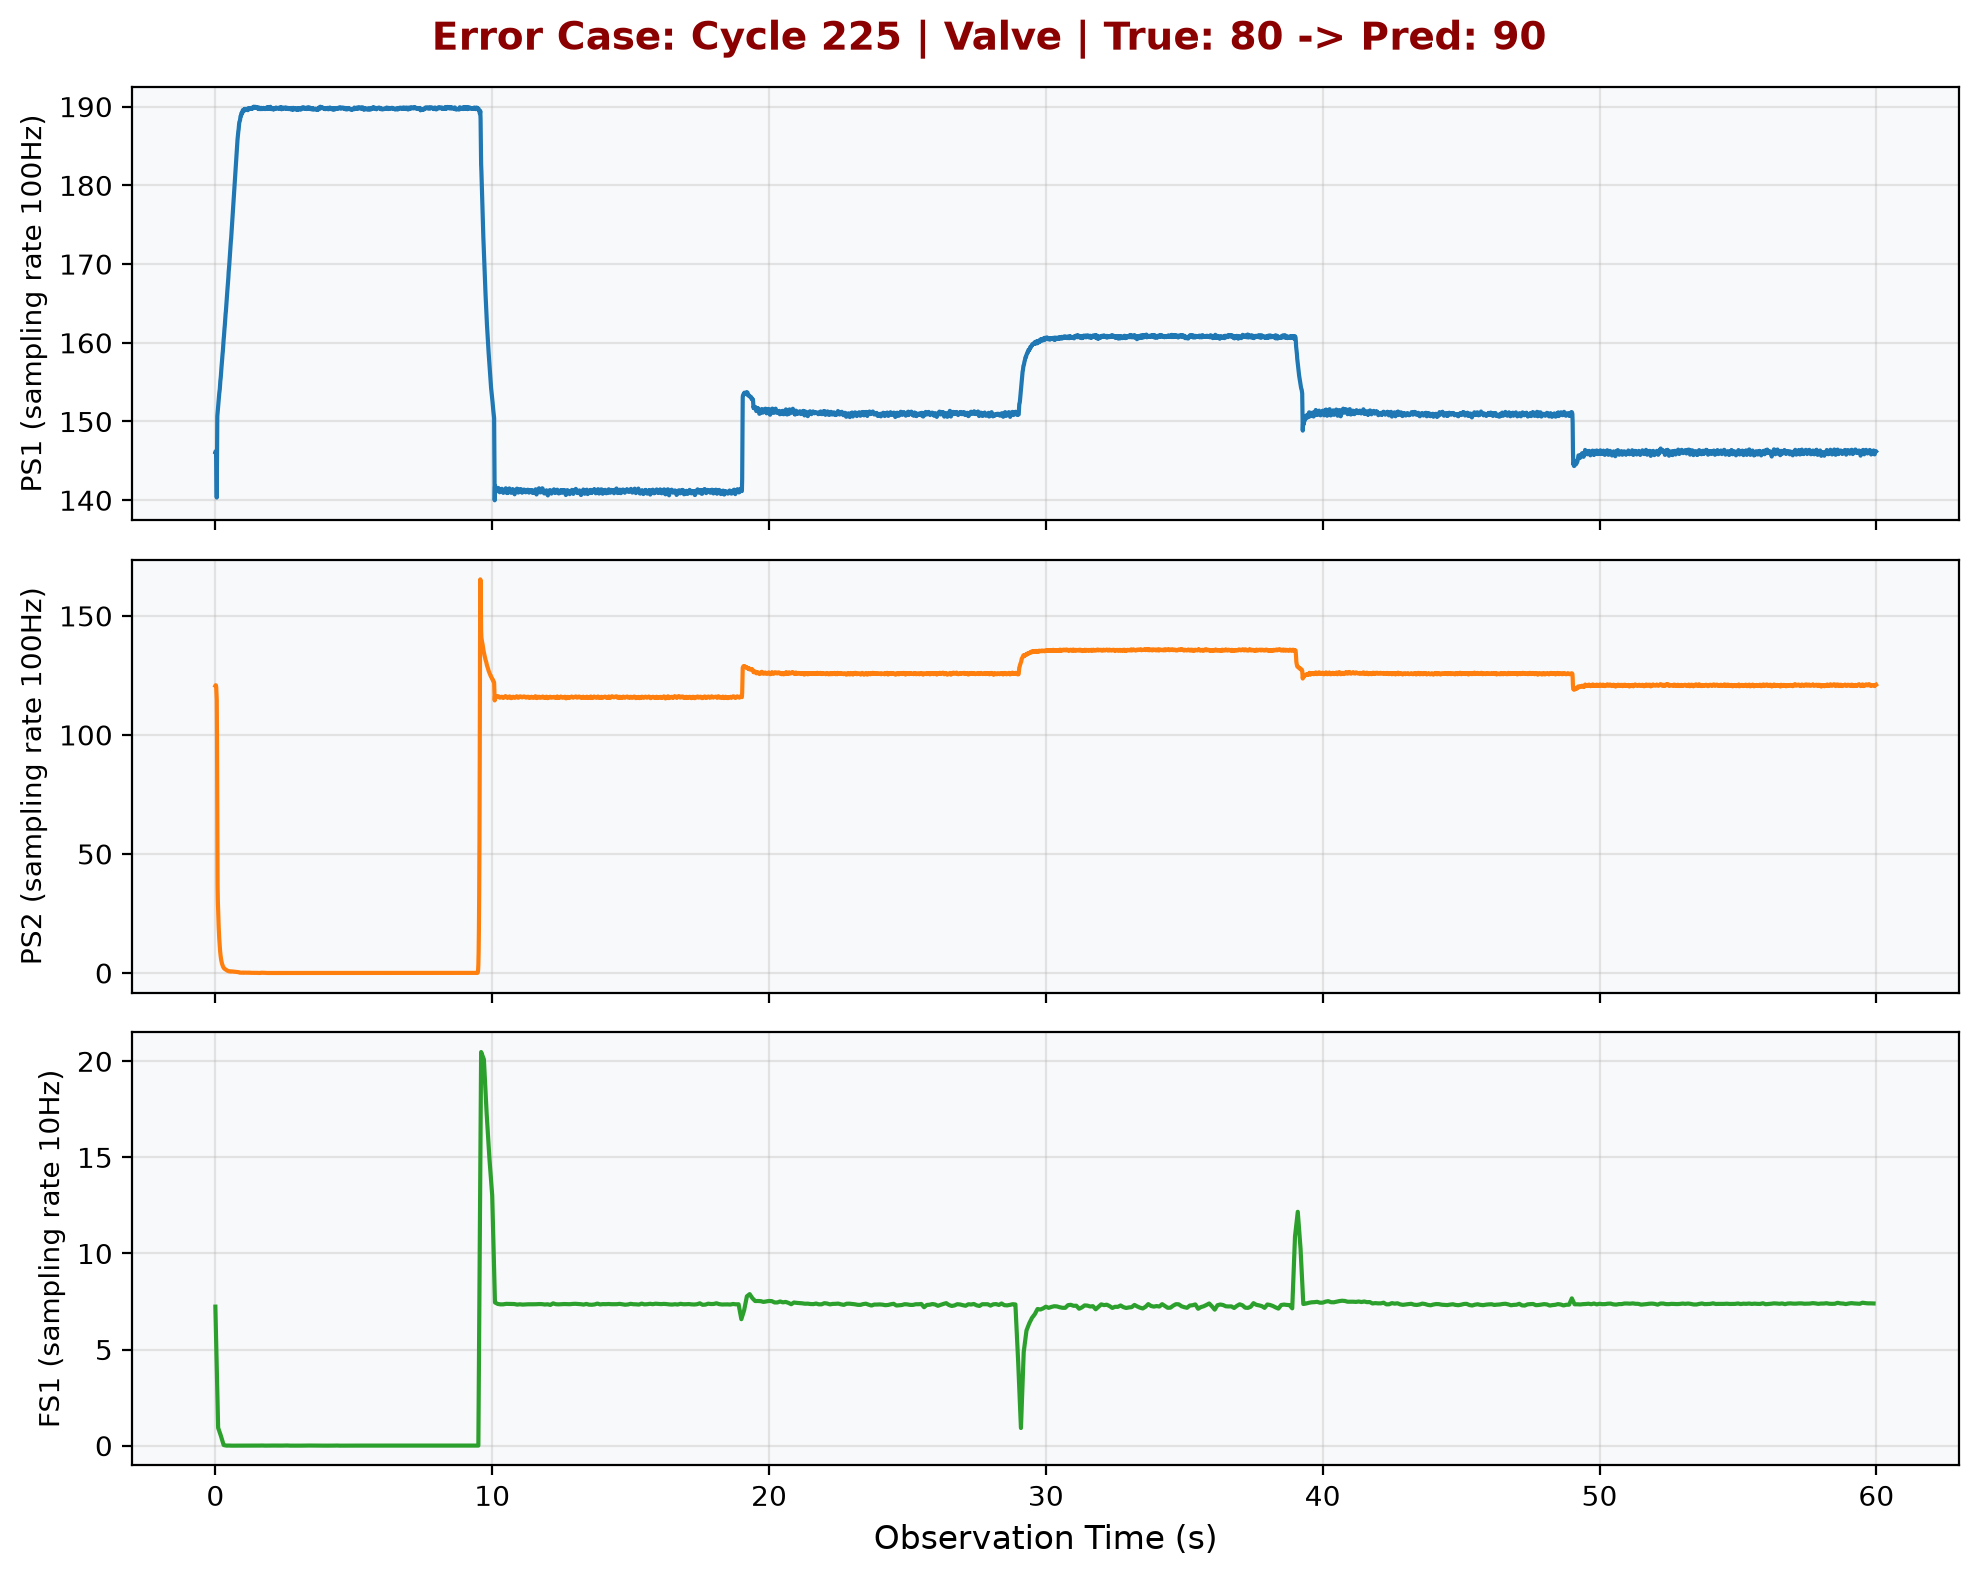
\includegraphics[width=0.5\linewidth]{figures/analysis_cycle_225.png}
  \caption{阀门滞后等级边界误判（Cycle 225，观测时长60s）。自上而下依次为：
  PS1 主系统压力（单位 bar）、PS2 控制压力（单位 bar）、FS1 系统流量（单位 L/min）。
  真实标签 80（严重滞后），预测标签 90（轻微滞后）。}
  \label{fig:err_cycle225}
\end{figure}
对于314周期错误样例如下图。波形中PS5/PS6蓄能器出口压力在8.42-8.53bar区间剧烈波动，整体标准差达到0.02bar，远高于正常130bar样本的平均0.008bar水平，但PS1主油路压力波形完全正常，无系统级压力异常。错判原因在于该误判由‌传感器噪声/工况瞬时波动‌导致：本周期蓄能器压力回路存在高频测量噪声，压力方差特征与115bar轻微泄漏时保压不足、压力脉动增大的故障特征完全重合；模型基于全局统计量判断，无法区分真实泄漏导致的压力脉动和传感器或者工况扰动导致的压力波动，因此误判为泄漏。
\begin{figure}[H]
  \centering
  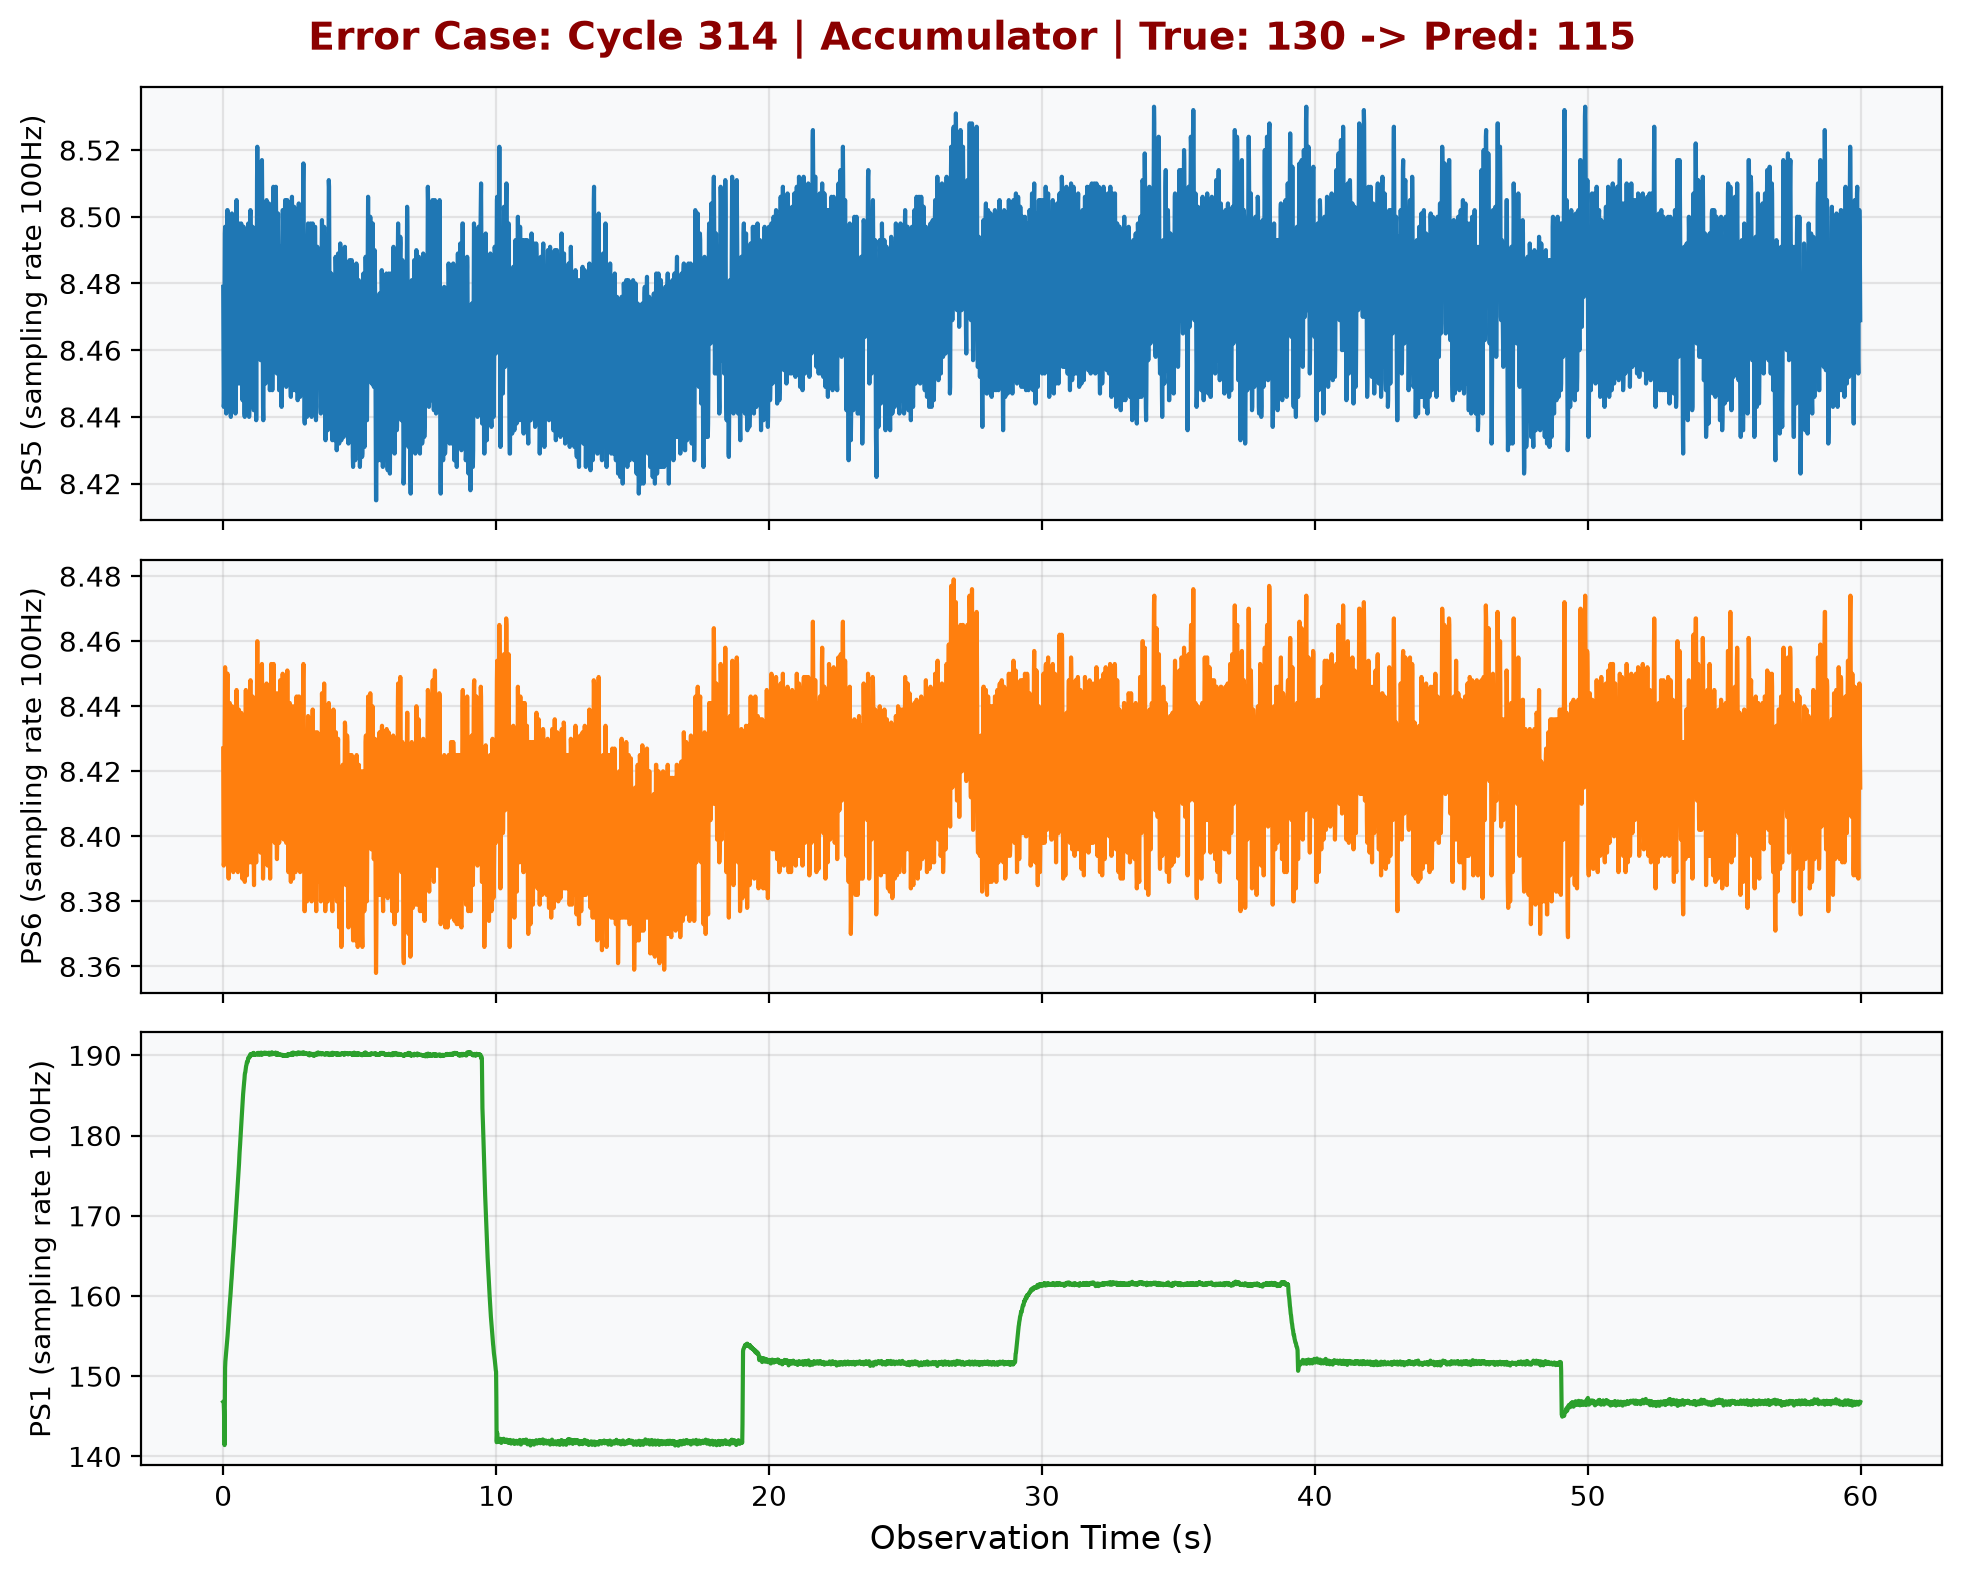
\includegraphics[width=0.5\linewidth]{figures/analysis_cycle_314.png}
  \caption{蓄能器压力脉动导致的误判（Cycle 314，观测时长60s）。自上而下依次为：
  PS5 蓄能器出口压力（单位 bar）、PS6 蓄能器出口压力（单位 bar）、PS1 主系统压力（单位 bar）。
  真实标签 130（预充压正常），预测标签 115（轻微泄漏）。}
  \label{fig:err_cycle314}
\end{figure}
对于629周期错误样例如下图。波形中10秒、30秒、50秒三个阀切换时刻FS1流量均出现接近20L/min的大幅尖峰，尖峰宽度约1秒；10-20s低压工作段FS1平均流量7.6L/min，EPS1平均功率2200W，恰好位于轻微泄漏与严重泄漏的特征区间分界处。错判原因在于阀切换瞬态尖峰掩盖了持续泄漏特征‌：严重内泄漏的核心特征是低压段流量降低、高压段内泄漏增大，本周期阀切换的大流量尖峰持续1秒，恰好落在20秒分段窗口内，拉高了分段流量均值，使得流量特征看起来与轻微泄漏一致；当前特征没有剔除阀切换瞬态的冲击，将瞬态流量计入工作段平均，导致泄漏程度被低估。
\begin{figure}[H]
  \centering
  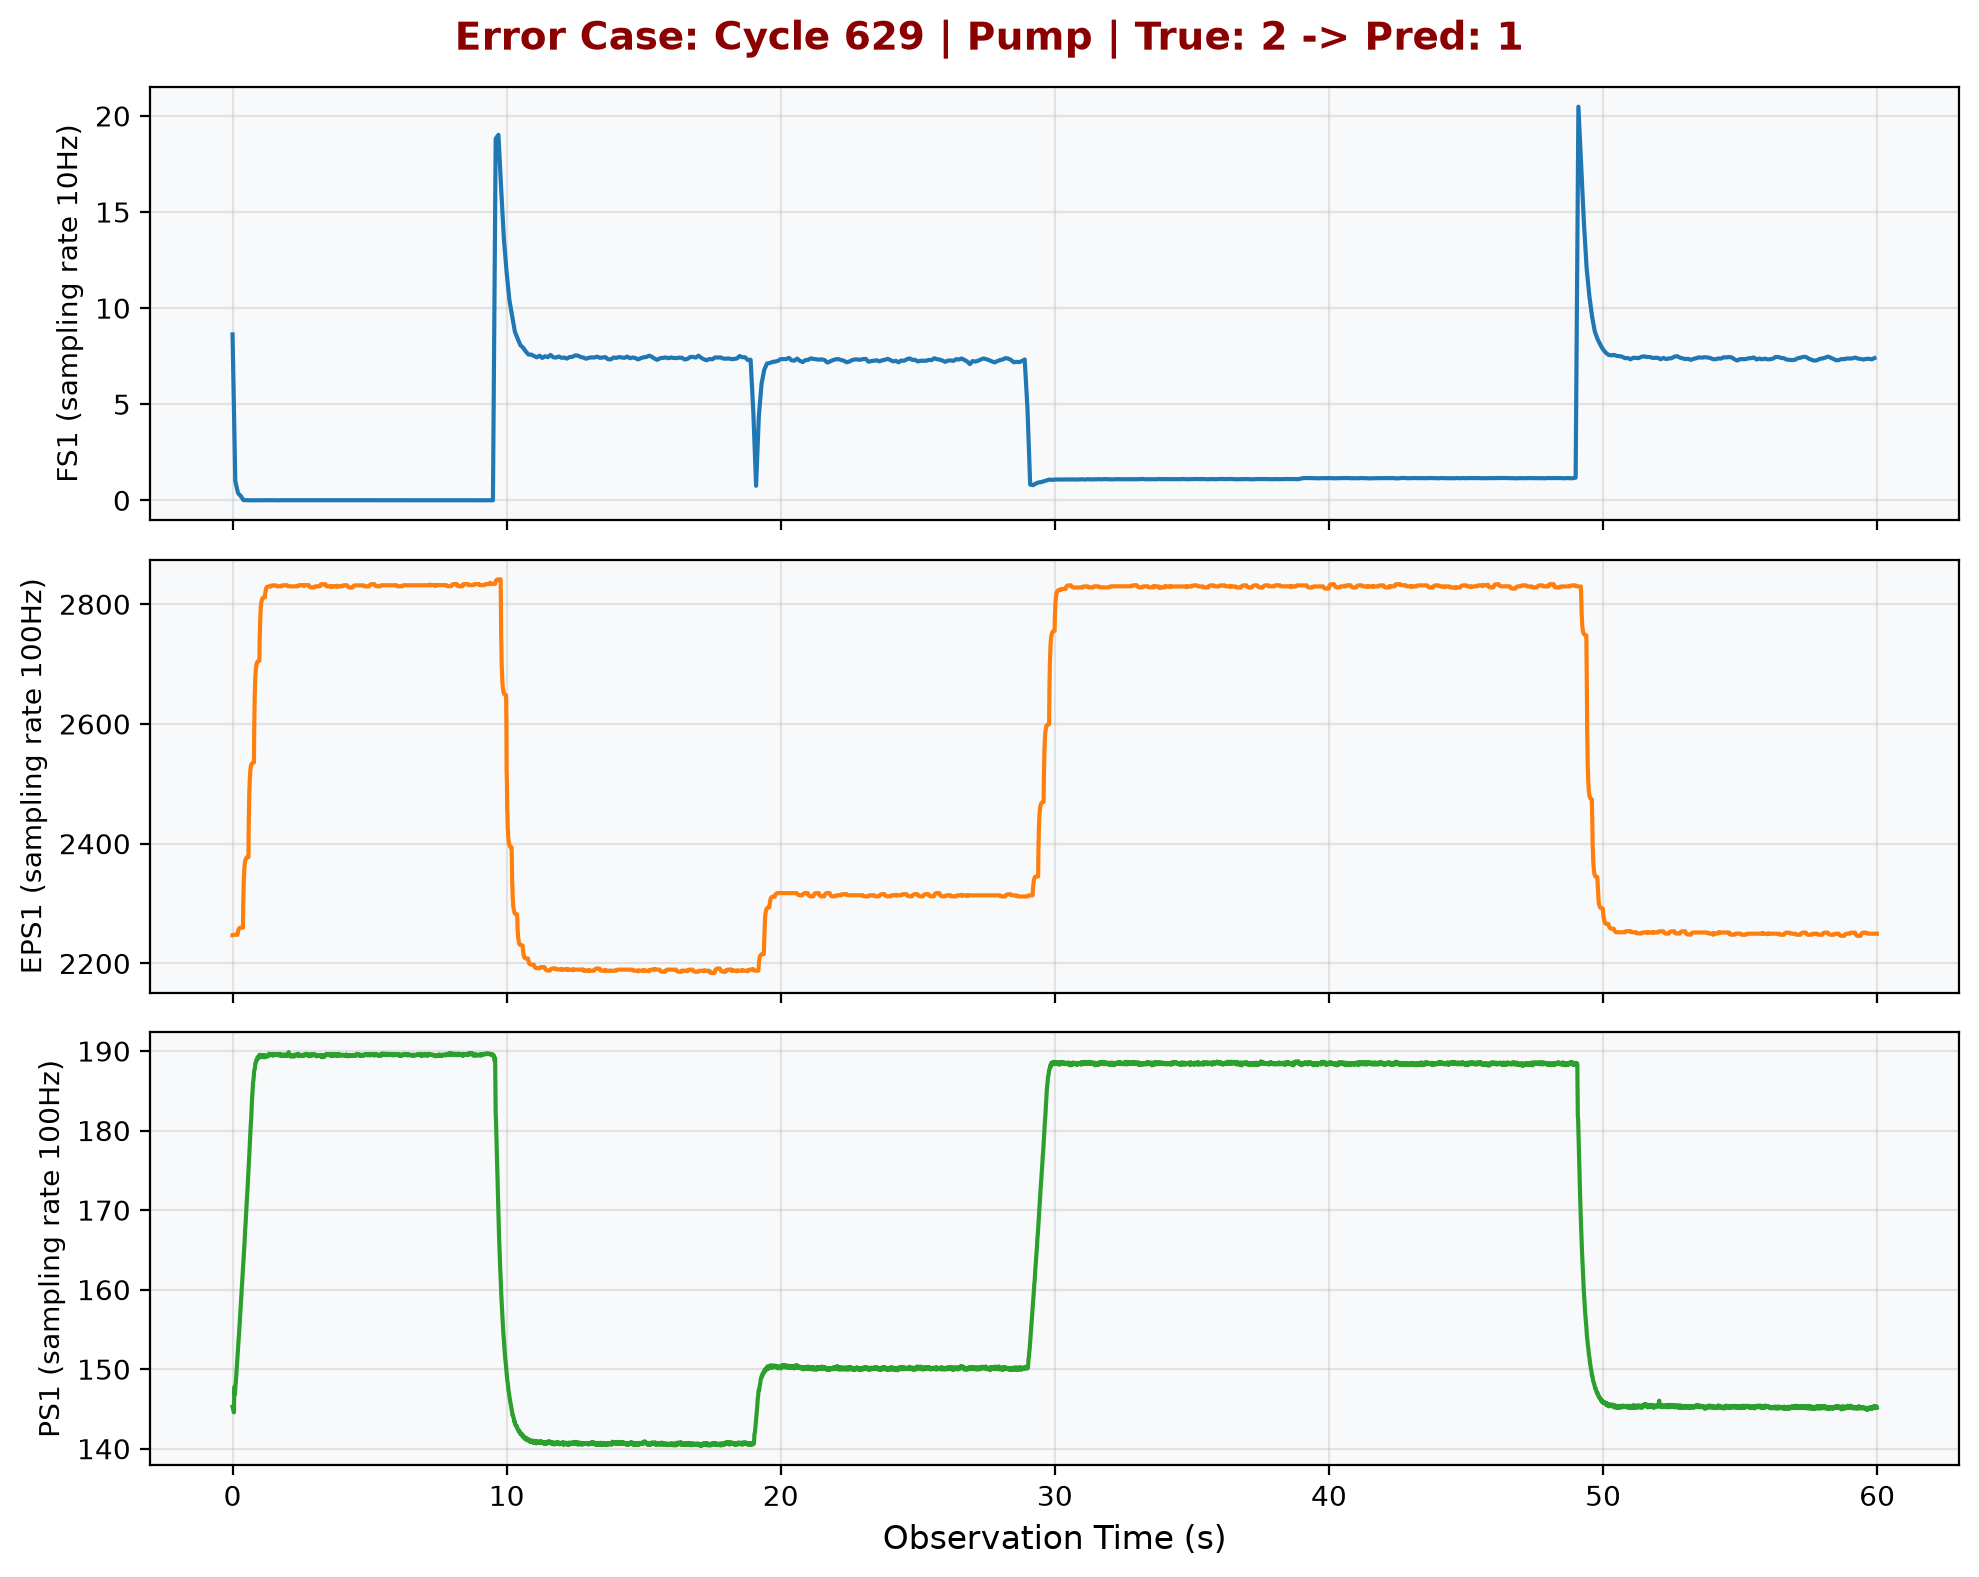
\includegraphics[width=0.5\linewidth]{figures/analysis_cycle_629.png}
  \caption{阀切换瞬态尖峰掩盖泵内泄漏程度（Cycle 629，观测时长60s）。自上而下依次为：
  FS1 系统流量（单位 L/min）、EPS1 电机功率（单位 W）、PS1 主系统压力（单位 bar）。
  真实标签 2（严重内泄漏），预测标签 1（轻微内泄漏）。}
  \label{fig:err_cycle629}
\end{figure}
对于1465周期错误样例如下图。波形中TS1进油温度从44.2℃线性下降至42.5℃，TS4出油温度从36.4℃线性下降至35.3℃，整周期进出油平均温差约7.8℃，远小于稳态正常冷却器的12℃温差，且温度线性斜率约为-0.03℃/s，属于典型的未热平衡状态。错判原因在于未稳定周期，本周期系统刚从高负载工况切换到低负载，油温处于持续回落过程，尚未达到热平衡；此时进出油温差小于稳态值，与冷却器效率下降、散热能力不足导致出油温度升高、温差变小的故障特征完全重合。模型仅学习了温差、温度均值等稳态特征，无法区分冷却器本身故障和系统未达到热平衡，因此出现误判。
\begin{figure}[H]
  \centering
  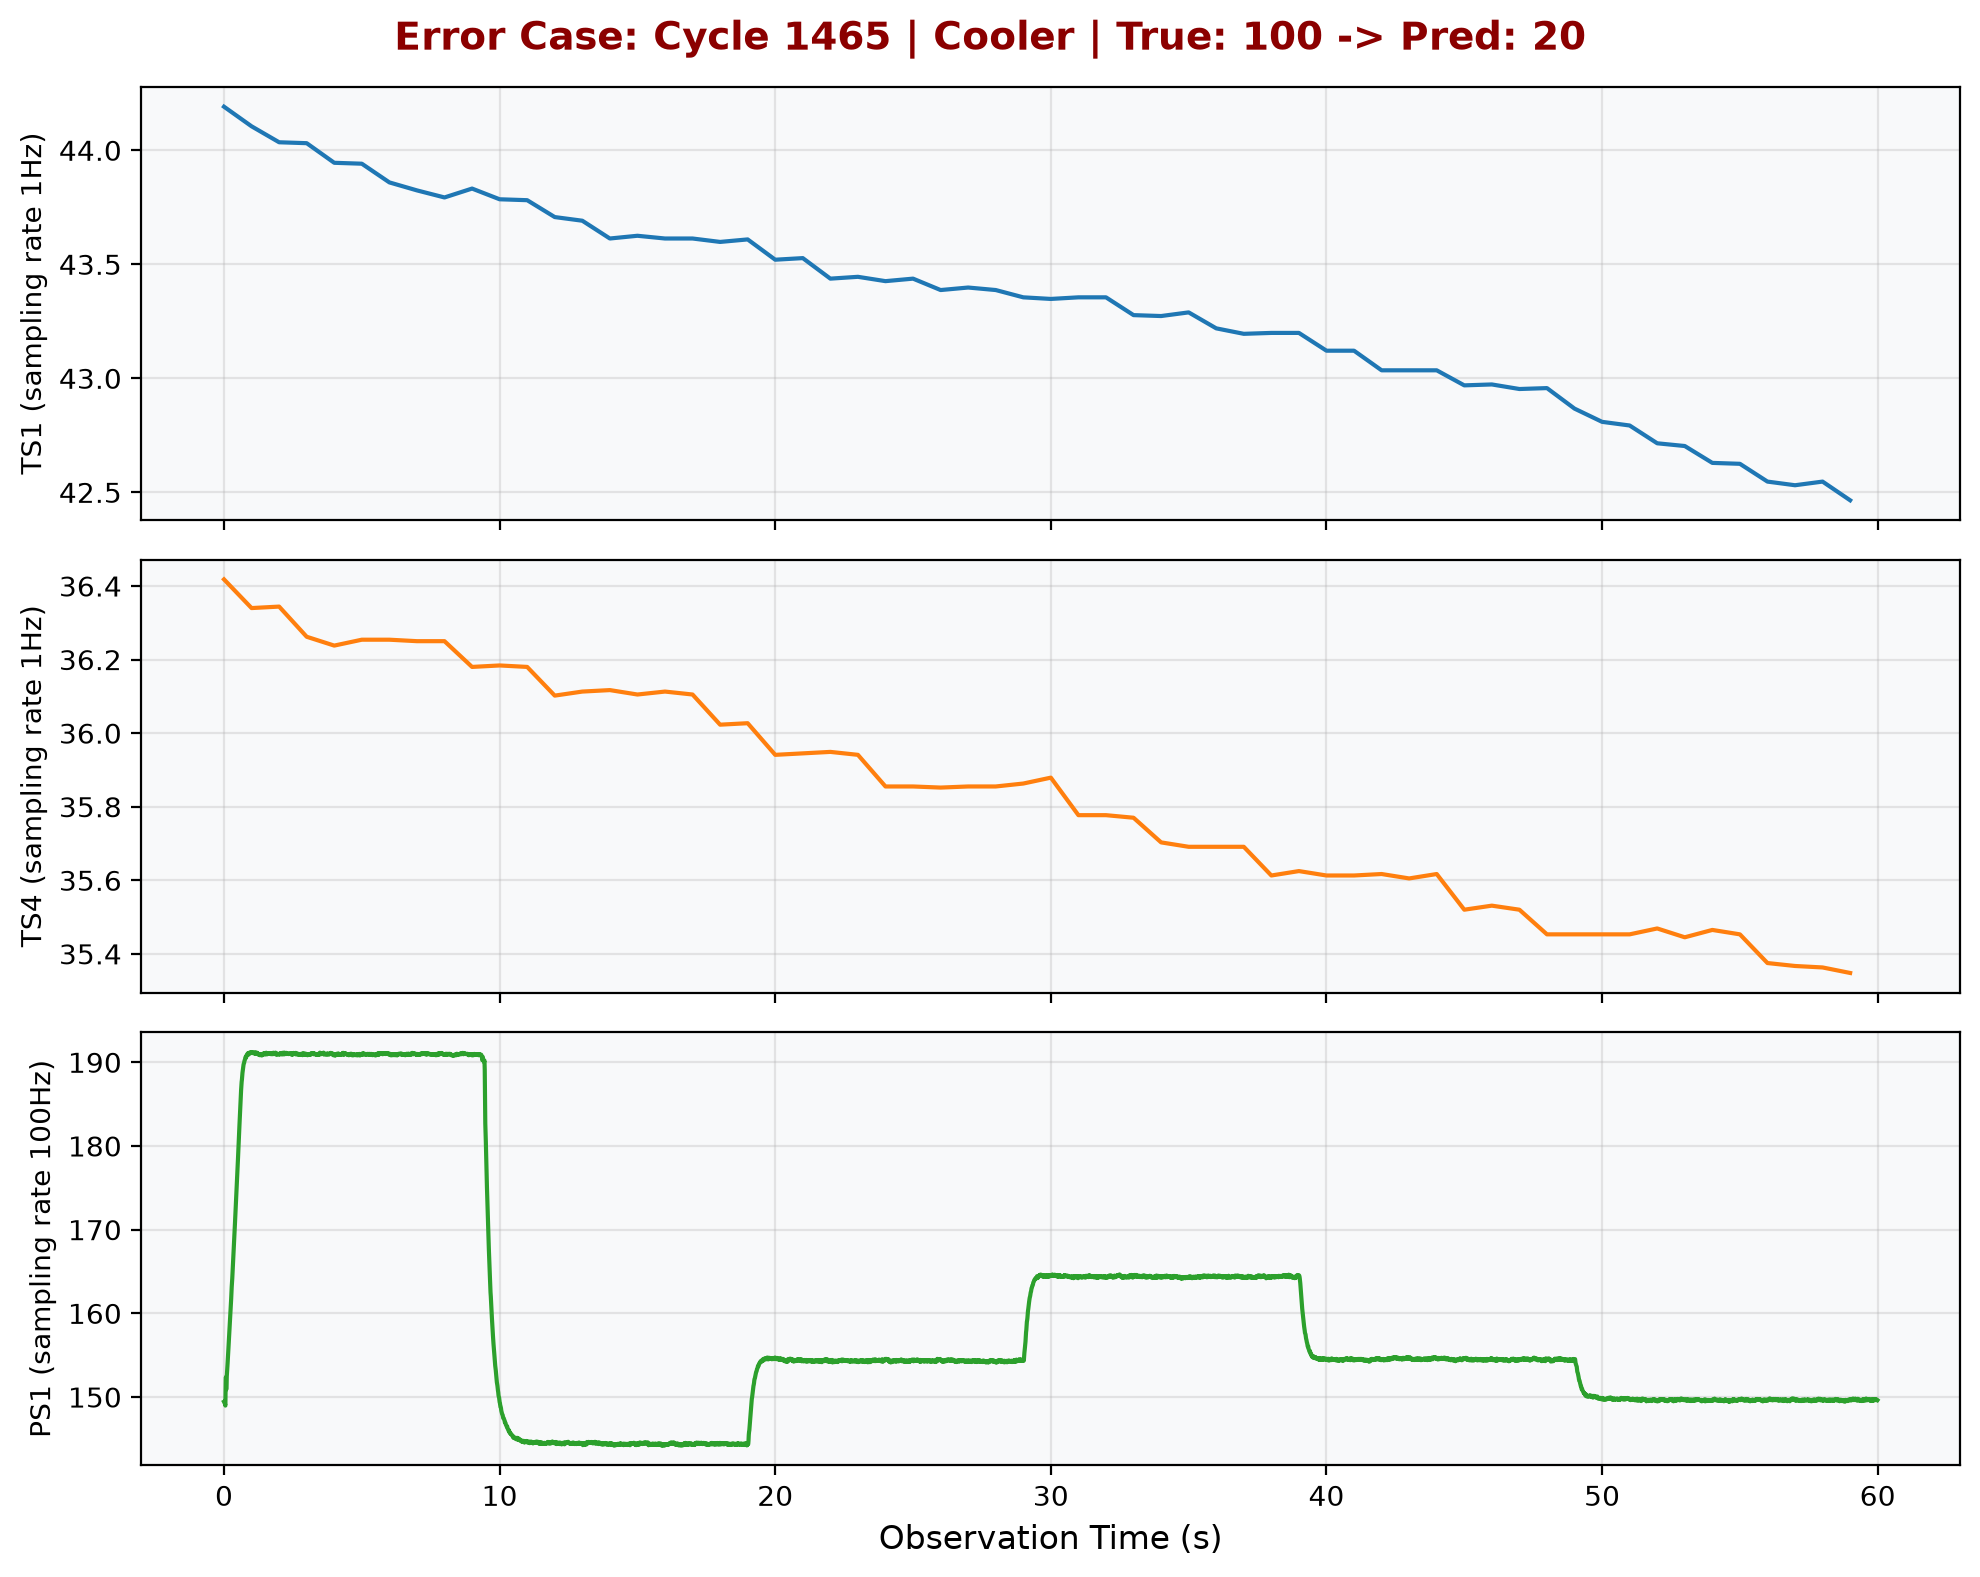
\includegraphics[width=0.5\linewidth]{figures/analysis_cycle_1465.png}
  \caption{未热平衡周期导致的冷却器误判（Cycle 1465，观测时长60s）。自上而下依次为：
  TS1 进油温度（单位 $^\circ$C）、TS4 出油温度（单位 $^\circ$C）、PS1 主系统压力（单位 bar）。
  真实标签 100（冷却效率正常），预测标签 20（效率严重下降）。}
  \label{fig:err_cycle1465}
\end{figure}
对于1546周期错误样例如下图。波形现象‌中10秒主切换沿陡度符合100最优阀门特征，但在18秒、28秒、48秒三个压力阶跃时刻，FS1均出现了2~3L/min的微小尖峰，压力切换时存在约0.1秒的轻微震荡。该误判来自‌个体制造公差/微小工况扰动‌：同一批次正常阀门的切换特性本身存在较小的个体波动，本周期的微小切换震荡属于正常公差范围，但当前模型决策边界对阀切换差分特征较为敏感，将正常范围内的切换震荡判定为轻微滞后；这类误判均为相邻等级的边界错误，没有出现跨等级的严重误判（如把100判为80严重滞后），不影响告警逻辑的正确性。
\begin{figure}[H]
  \centering
  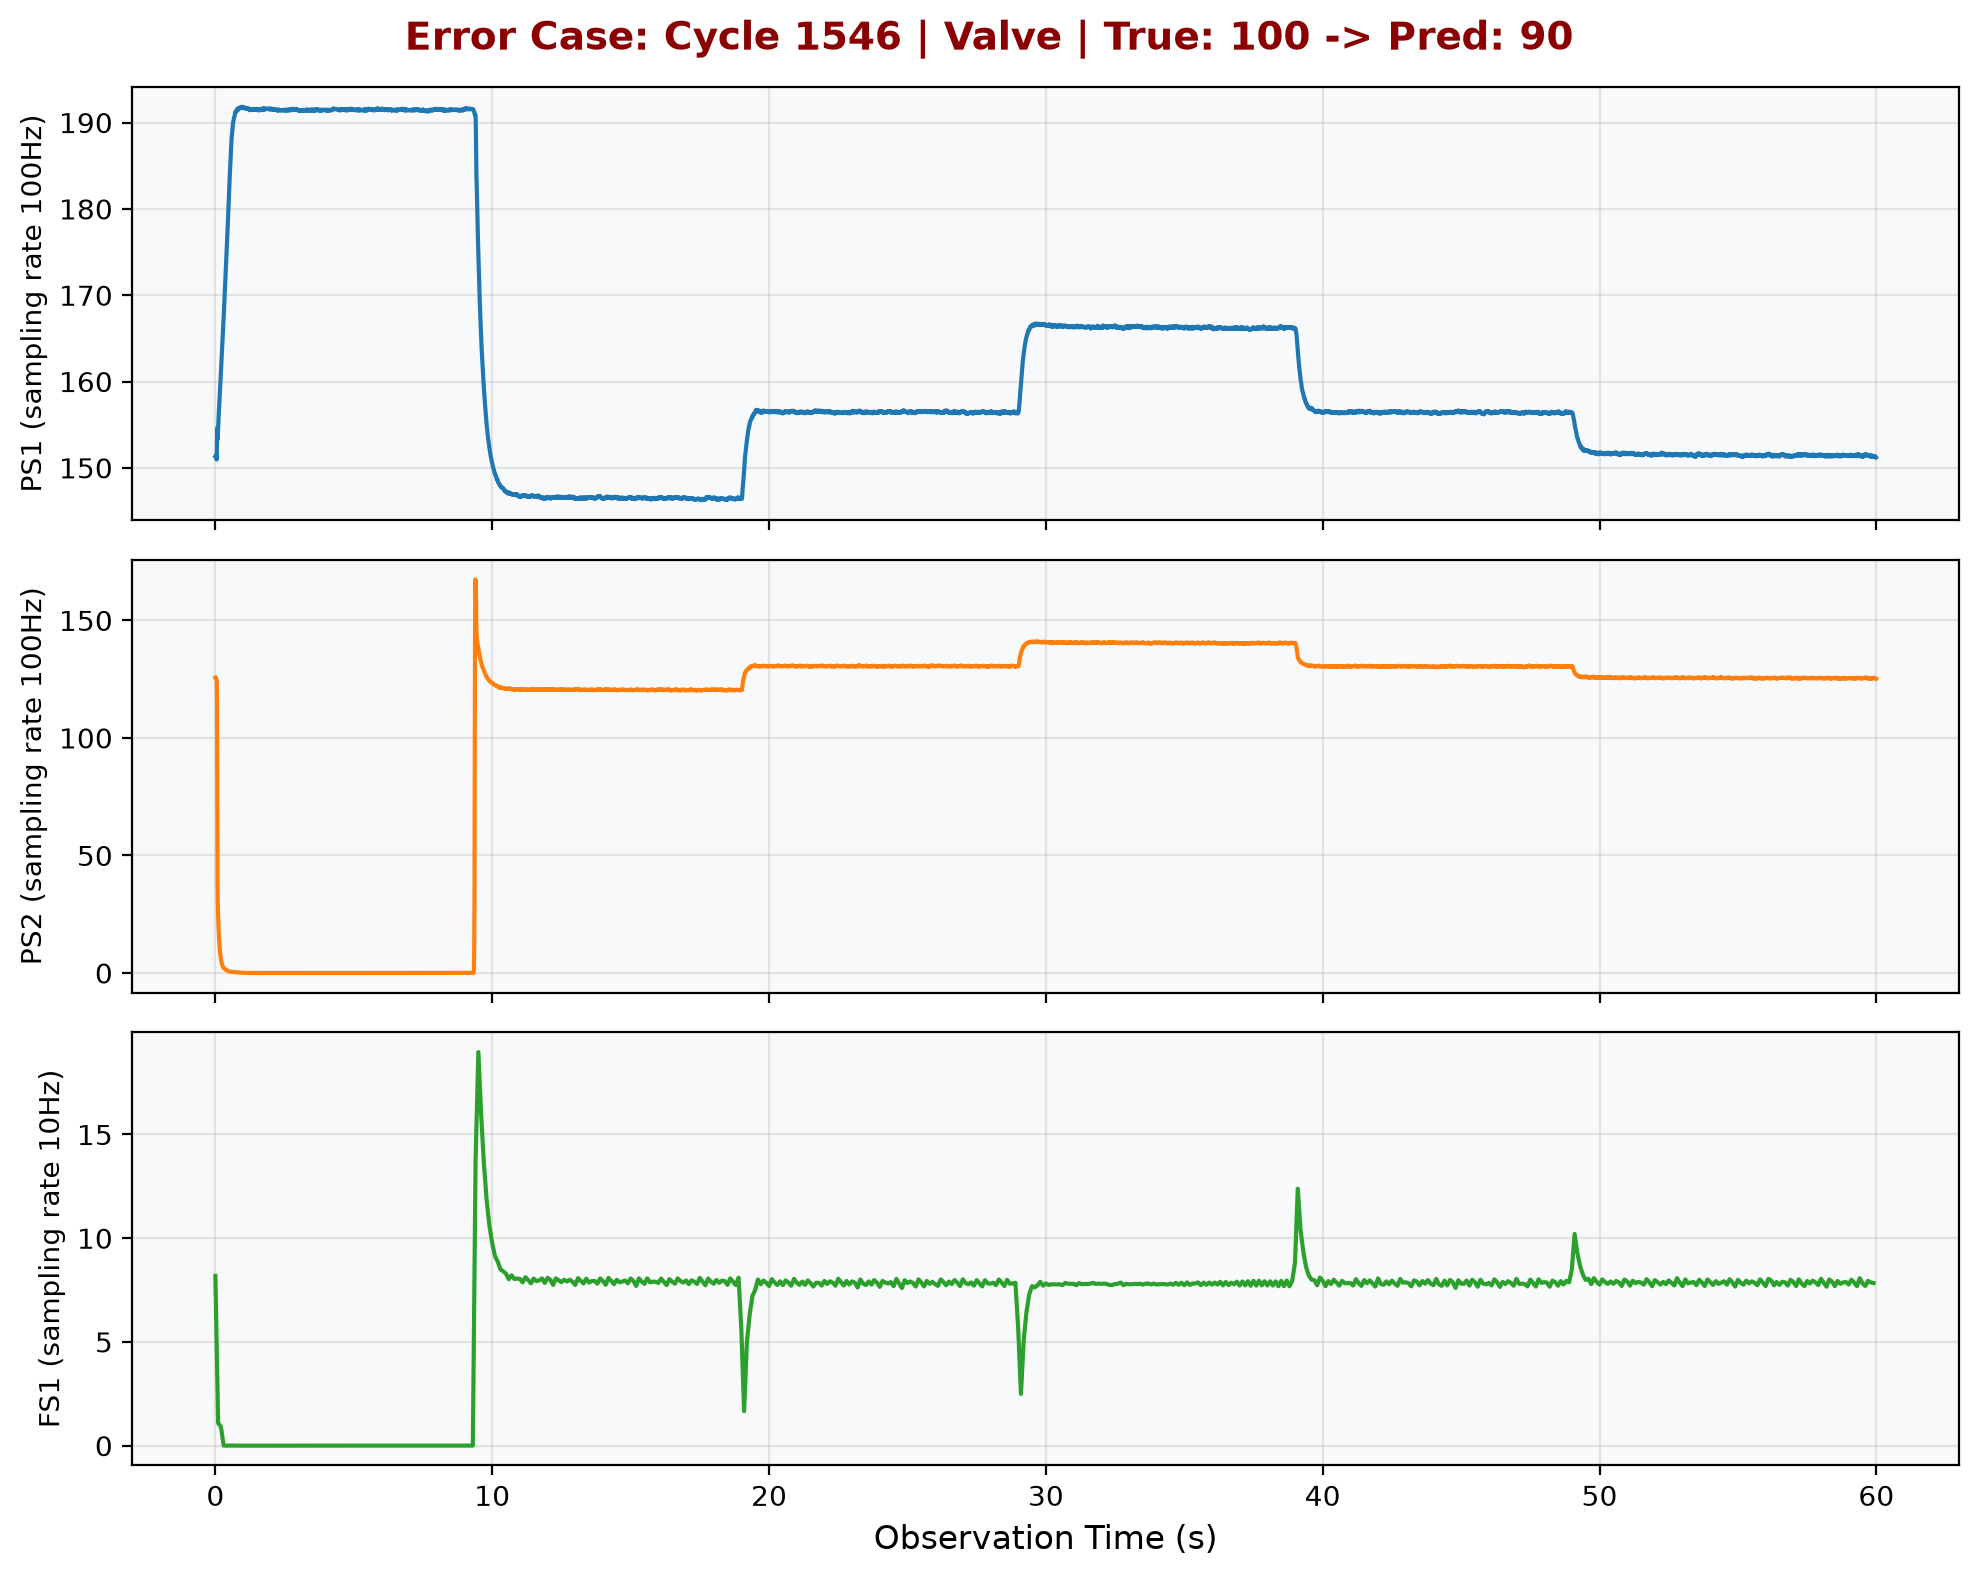
\includegraphics[width=0.5\linewidth]{figures/analysis_cycle_1546.png}
  \caption{个体公差范围内的切换震荡误判（Cycle 1546，观测时长60s）。自上而下依次为：
  PS1 主系统压力（单位 bar）、PS2 控制压力（单位 bar）、FS1 系统流量（单位 L/min）。
  真实标签 100（无滞后），预测标签 90（轻微滞后）。}
  \label{fig:err_cycle1546}
\end{figure}
\section{本地系统与回放}
\subsection{本地回放系统}
本系统提供本地回放脚本replay.py，支持按源周期时间依次推进单个负载周期，用于现场演示诊断与告警过程。回放界面在2*2子图中同步展示压力（PS1）、流量（FS1）、温度（TS1）与振动（VS1）四路代表通道的波形：蓝线为当前时点已观测到的时间前缀，随源时间在10、30、60秒三个时点逐步扩展；每个时点均在终端输出四个部件各自的诊断等级、类别得分与异常候选状态，并标注当前缺失或掉线的传感器通道（如屏蔽FS1时在对应子图提示SENSOR OFFLINE）。系统支持正常与加速两种回放倍率，切换周期后清空历史候选与告警状态，保证各周期相互独立。

回放严格遵循因果约束：在某时点的诊断只使用该时刻之前已经到达的信号前缀，未来信号不参与特征计算与预测；回放倍率的变化不改变任何单周期的诊断结论。周期真值标签仅供独立评测与事后分析使用，不进入诊断输入与实时显示。

\subsection{输出文件与运行接口}
系统运行时产出四个结果文件，主要内容如下表所示。
\begin{table}[H]
  \centering
  \caption{系统输出文件与主要内容}
  \label{tab:outputs}
  \small
  \begin{tabular}{@{}p{3.0cm}p{10.8cm}@{}}
    \toprule
    \textbf{文件} & \textbf{主要内容} \\
    \midrule
    manifest.csv & 周期编号、四部件标签、组合编号（group\_id）、稳定性标志、所属集合（train/val/test）与原始行号，仅用于数据管理与评分。 \\
    \addlinespace
    predictions.csv & 周期编号、观测预算（10/30/60\,s）、部件、预测等级、类别得分、数据质量与方案及扰动条件。 \\
    \addlinespace
    alarms.json & 周期编号、部件、首次正式告警时间、当时告警等级、候选时间、最终等级以及告警后的更新记录。 \\
    \addlinespace
    metrics.json & 逐部件 Macro-F1 与逐等级 Recall、严格联合准确率、异常定位、告警指标、稳定性分层、扰动与性能结果及配置。 \\
    \bottomrule
  \end{tabular}
\end{table}

本地运行接口示例如下：
\begin{lstlisting}[language=bash, caption=本地运行接口示例]
python prepare.py 
python train_b0.py
python replay.py --cycle 100 --model b1 --speed normal
python evaluate.py
\end{lstlisting}
本系统全部基本功能均可在 CPU 上完成，不依赖 GPU，亦不要求网页或工业控制接口。

\section{局限与展望}
\subsection{系统目前局限}
标签粒度造成不可约的边界误差。目前每个部件仅有4到5个离散等级，相邻等级在波形上表现差距很小，多个错误展现此种相邻等级误判，属于数据本身的可分性上界，更换模型可能也无法消除。

使用静态特征压缩了周期内的动态过程。当前系统将整个60秒周期折叠成一个特征向量，保留其均值、标准差与分段差分等统计量，可能导致严重的瞬态变化被分段均值稀释问题，不适用于动态变化的部件进行诊断。

引入物理交叉特征只在特定部件上有效，并在传感器整体掩蔽的情况下完全失效，说明添加物理交叉特征的模型会对单一特定物理量通道高度依赖，缺乏冗余，一旦该通道失效诊断易失败。

目前使用评估设计较单一，仅使用固定测试与训练集划分，未完成交叉验证，扰动鲁棒性条件覆盖退化种类较少，跨设备、跨工况的泛化能力尚未验证。
\subsection{系统未来展望}
后续考虑引入时序建模，使用长短期记忆网络或一维卷积直接在原始序列上学习，保留周期内的演化过程，可望修复被均值抹平的瞬态误判。

补充瞬态和频域特征，提取切换沿斜率、上升时间、小波变换能量、频域谱等亚秒级特征，补齐分段统计对瞬态不敏感的短板。

对于多分类问题转换为序数回归，相邻等级误判的代价远小于跨等级误判，用序数回归或多标签严重度评分替代独立分类，更贴合实际诊断需求。
\begin{thebibliography}{9}
\bibitem{helwig2015} Helwig, N., Pignanelli, E., \& Schütze, A. (2015). \textit{Condition monitoring of hydraulic systems}. UCI Machine Learning Repository. DOI: 10.24432/C5CW21. 许可：CC BY 4.0（传感器、等级与单位以官方说明及原始发布文件为准）。
\end{thebibliography}

\subsection*{开源工具与辅助说明}
本项目在 Python 3.12.16 环境下实现，主要依赖的开源库及其版本为：numpy 2.5.4、pandas 3.1.1、scikit-learn 1.9.1、scipy 1.18.1、matplotlib 3.11.2、joblib 1.6.0。四部件分类器采用 scikit-learn 的 RandomForestClassifier（n\_estimators=200，random\_state=2026）。上述开源库均为未经修改的原始发布版本，本项目仅在其基础上编写数据处理、特征工程、训练、评测与回放脚本。

关于人工智能辅助工具：本报告在文字撰写、\LaTeX 排版与代码调试环节使用了人工智能辅助工具（VSCode中的AI编程助手），用于辅助措辞、排查报错与整理格式。数据的读取与质量检查、固定的状态组合划分、特征工程、B0/B1/B2方案设计、鲁棒性实验、全部指标计算与结果分析使用人工智能辅助工具进行指导辅助；未使用测试集标签进行任何调参，亦未伪造或篡改实验数据。

\end{document}